\documentclass[a4paper]{scrartcl}
% Packages
\usepackage{stix}
\usepackage[margin=1.5in]{geometry}
\usepackage{index}
\makeindex
\usepackage[utf8]{inputenc}
\usepackage[T1]{fontenc}
\usepackage{varwidth}
\usepackage{amsmath, amssymb}
\usepackage{esint}
\usepackage{titlesec}
\usepackage{xcolor}
\usepackage{titling}
\usepackage{tensor}
\usepackage[linktocpage]{hyperref}
\usepackage{pgfplots}
\usepackage{multicol}
\setlength{\columnsep}{2em}
\usepackage{caption}
\usepackage{amsthm}
\usepackage{import}
\usepackage{cancel}
\usepackage{caption}
\usepackage{tcolorbox}
\usepackage{nicematrix}
\usepackage{mathrsfs}
\usepackage{mathtools}
\usepackage{enumerate}
\usepackage{graphicx}
\usepackage{lipsum}
\usepackage[italian]{babel}
\usepackage{setspace}
\setstretch{1.2}


%Captions
\captionsetup[figure]{font=footnotesize,labelfont=footnotesize}
\captionsetup[table]{font=footnotesize,labelfont=footnotesize}
%Titlesec
\titleformat{\section}
{\fontsize{18}{20}\sffamily\scshape}
{\normalfont\color{gray}{\fontsize{22}{20}\selectfont\thesection}}
{0.7em}
{}
\hypersetup{colorlinks,breaklinks, linkcolor=[RGB]{74, 122, 164}}

\newcommand\vertarrowbox[3][6ex]{%
  \begin{array}[t]{@{}c@{}} #2 \
  \left\uparrow\vcenter{\hrule height #1}\right.\kern-\nulldelimiterspace\
  \makebox[0pt]{\scriptsize#3}
  \end{array}%
}
\definecolor{asdf}{HTML}{4a7aa4}
% Personalizza la formattazione della subsection
\titleformat{\subsection}[block]{\fontsize{14}{20}\bfseries}{\normalfont\thesubsection}{.5em}{}


% Personalizza la formattazione della subsubsection
\titleformat{\subsubsection}[block]{\fontsize{12}{20}\bfseries}{\normalfont\thesubsubsection}{.5em}{}

% Maketitle customization
\renewcommand{\maketitle}{
\begin{center}
{\sffamily
{\fontsize{20}{20}\selectfont\MakeUppercase\thetitle}}

\vspace{0.2in}

{\large\scshape\sffamily\theauthor}
\end{center}
}

% Titles 
\title{Note di Fisica 2}
\author{Manuel Deodato}
\date{}



%Evaluate symbol
\DeclareMathOperator{\di}{d\!}
\newcommand*\Eval[3]{\left.#1\right\rvert_{#2}^{#3}}

%%%%%%% Numero delle equazioni in formato a.b
\numberwithin{equation}{subsection}
%%%%%

%%%%%%%%%% Personalizzazione numeri lista
\renewcommand{\theenumi}{(\arabic{enumi})}

%%%%%%%%%% Medie con integrali multipli
\def\Yint#1{\mathchoice
    {\YYint\displaystyle\textstyle{#1}}%
    {\YYint\textstyle\scriptstyle{#1}}%
    {\YYint\scriptstyle\scriptscriptstyle{#1}}%
    {\YYint\scriptscriptstyle\scriptscriptstyle{#1}}%
      \!\iint}
\def\YYint#1#2#3{{\setbox0=\hbox{$#1{#2#3}{\iint}$}
    \vcenter{\hbox{$#2#3$}}\kern-.51\wd0}}
\def\longdash{{-}\mkern-3.5mu{-}} 
   % consider using "\mkern-7.5mu" if esint package is loaded
\def\tiltlongdash{\rotatebox[origin=c]{15}{$\longdash$}}
\def\fiint{\Yint\tiltlongdash}

\def\Zint#1{\mathchoice
    {\YYint\displaystyle\textstyle{#1}}%
    {\YYint\textstyle\scriptstyle{#1}}%
    {\YYint\scriptstyle\scriptscriptstyle{#1}}%
    {\YYint\scriptscriptstyle\scriptscriptstyle{#1}}%
      \!\iiint}
      \def\tilongdash{\mkern6mu{-}\mkern-4mu{-}\mkern-5mu{-}} 
   % consider using "\mkern-7.5mu" if esint package is loaded
\def\titiltlongdash{\rotatebox[origin=c]{15}{$\tilongdash$}}
\def\fiiint{\Zint\titiltlongdash}


%%%% Table of contents

\usepackage[titles]{tocloft}

\renewcommand{\cftdot}{}
\usepackage{titletoc}
%\setcounter{tocdepth}{2}

%%%%%%%%%%%%%%%% Toc style

% Personalizzazione scritta indice


% Font
\usepackage[osf]{newpxtext}

\usepackage{sansiwona}


% Ambienti
\newtheoremstyle{style1}% name of the style to be used
{15pt}% measure of space to leave above the theorem. E.g.: 3pt
{15pt}% measure of space to leave below the theorem. E.g.: 3pt
{\normalfont}% name of font to use in the body of the theorem
{}% measure of space to indent
{\sffamily\scshape\bfseries}% name of head font
{}% punctuation between head and body
{ }% space after theorem head; " " = normal interword space
{\thmname{#1}\thmnumber{ #2}{\thmnote{~--- #3}}.\newline}




\theoremstyle{style1}
\newtheorem{teorema}{Teorema}[section]
\newtheorem{corollario}{Corollario}[teorema]
\newtheorem{lemma}{Lemma}[teorema]
\newtheorem{definizione}{Definizione}[section]
\newtheorem{osservazione}{Osservazione}[section]
\newtheorem{notazione}{Notazione}[section]
\newtheorem{esempio}{Esempio}[section]
\newtheorem{esercizio}{Esercizio}[section]

\renewcommand\qedsymbol{$\blacksquare$}

\newenvironment{svolgimento}{\renewcommand\qedsymbol{$\spadesuit$}\begin{proof}[Svolgimento]}{\end{proof}}

%% Generic box
\newtcolorbox{eqbox}[1][]
{
colback=gray!10,
arc=0pt,
boxrule=0pt,
title=#1
}

 \newenvironment{boxenv}[1][]{
    \begin{eqbox}[#1]
    }{
   \end{eqbox}
}








%%%%%%%%%%%%%%%%%%%%%%%%%%%%%%%%%%%%%%%%%%%%%%%%%%%%%%%%%%%%%%%%%%%%%%%%

\begin{document}
\maketitle
\vspace{9cm}
\begin{figure}[h!]
	\centering
	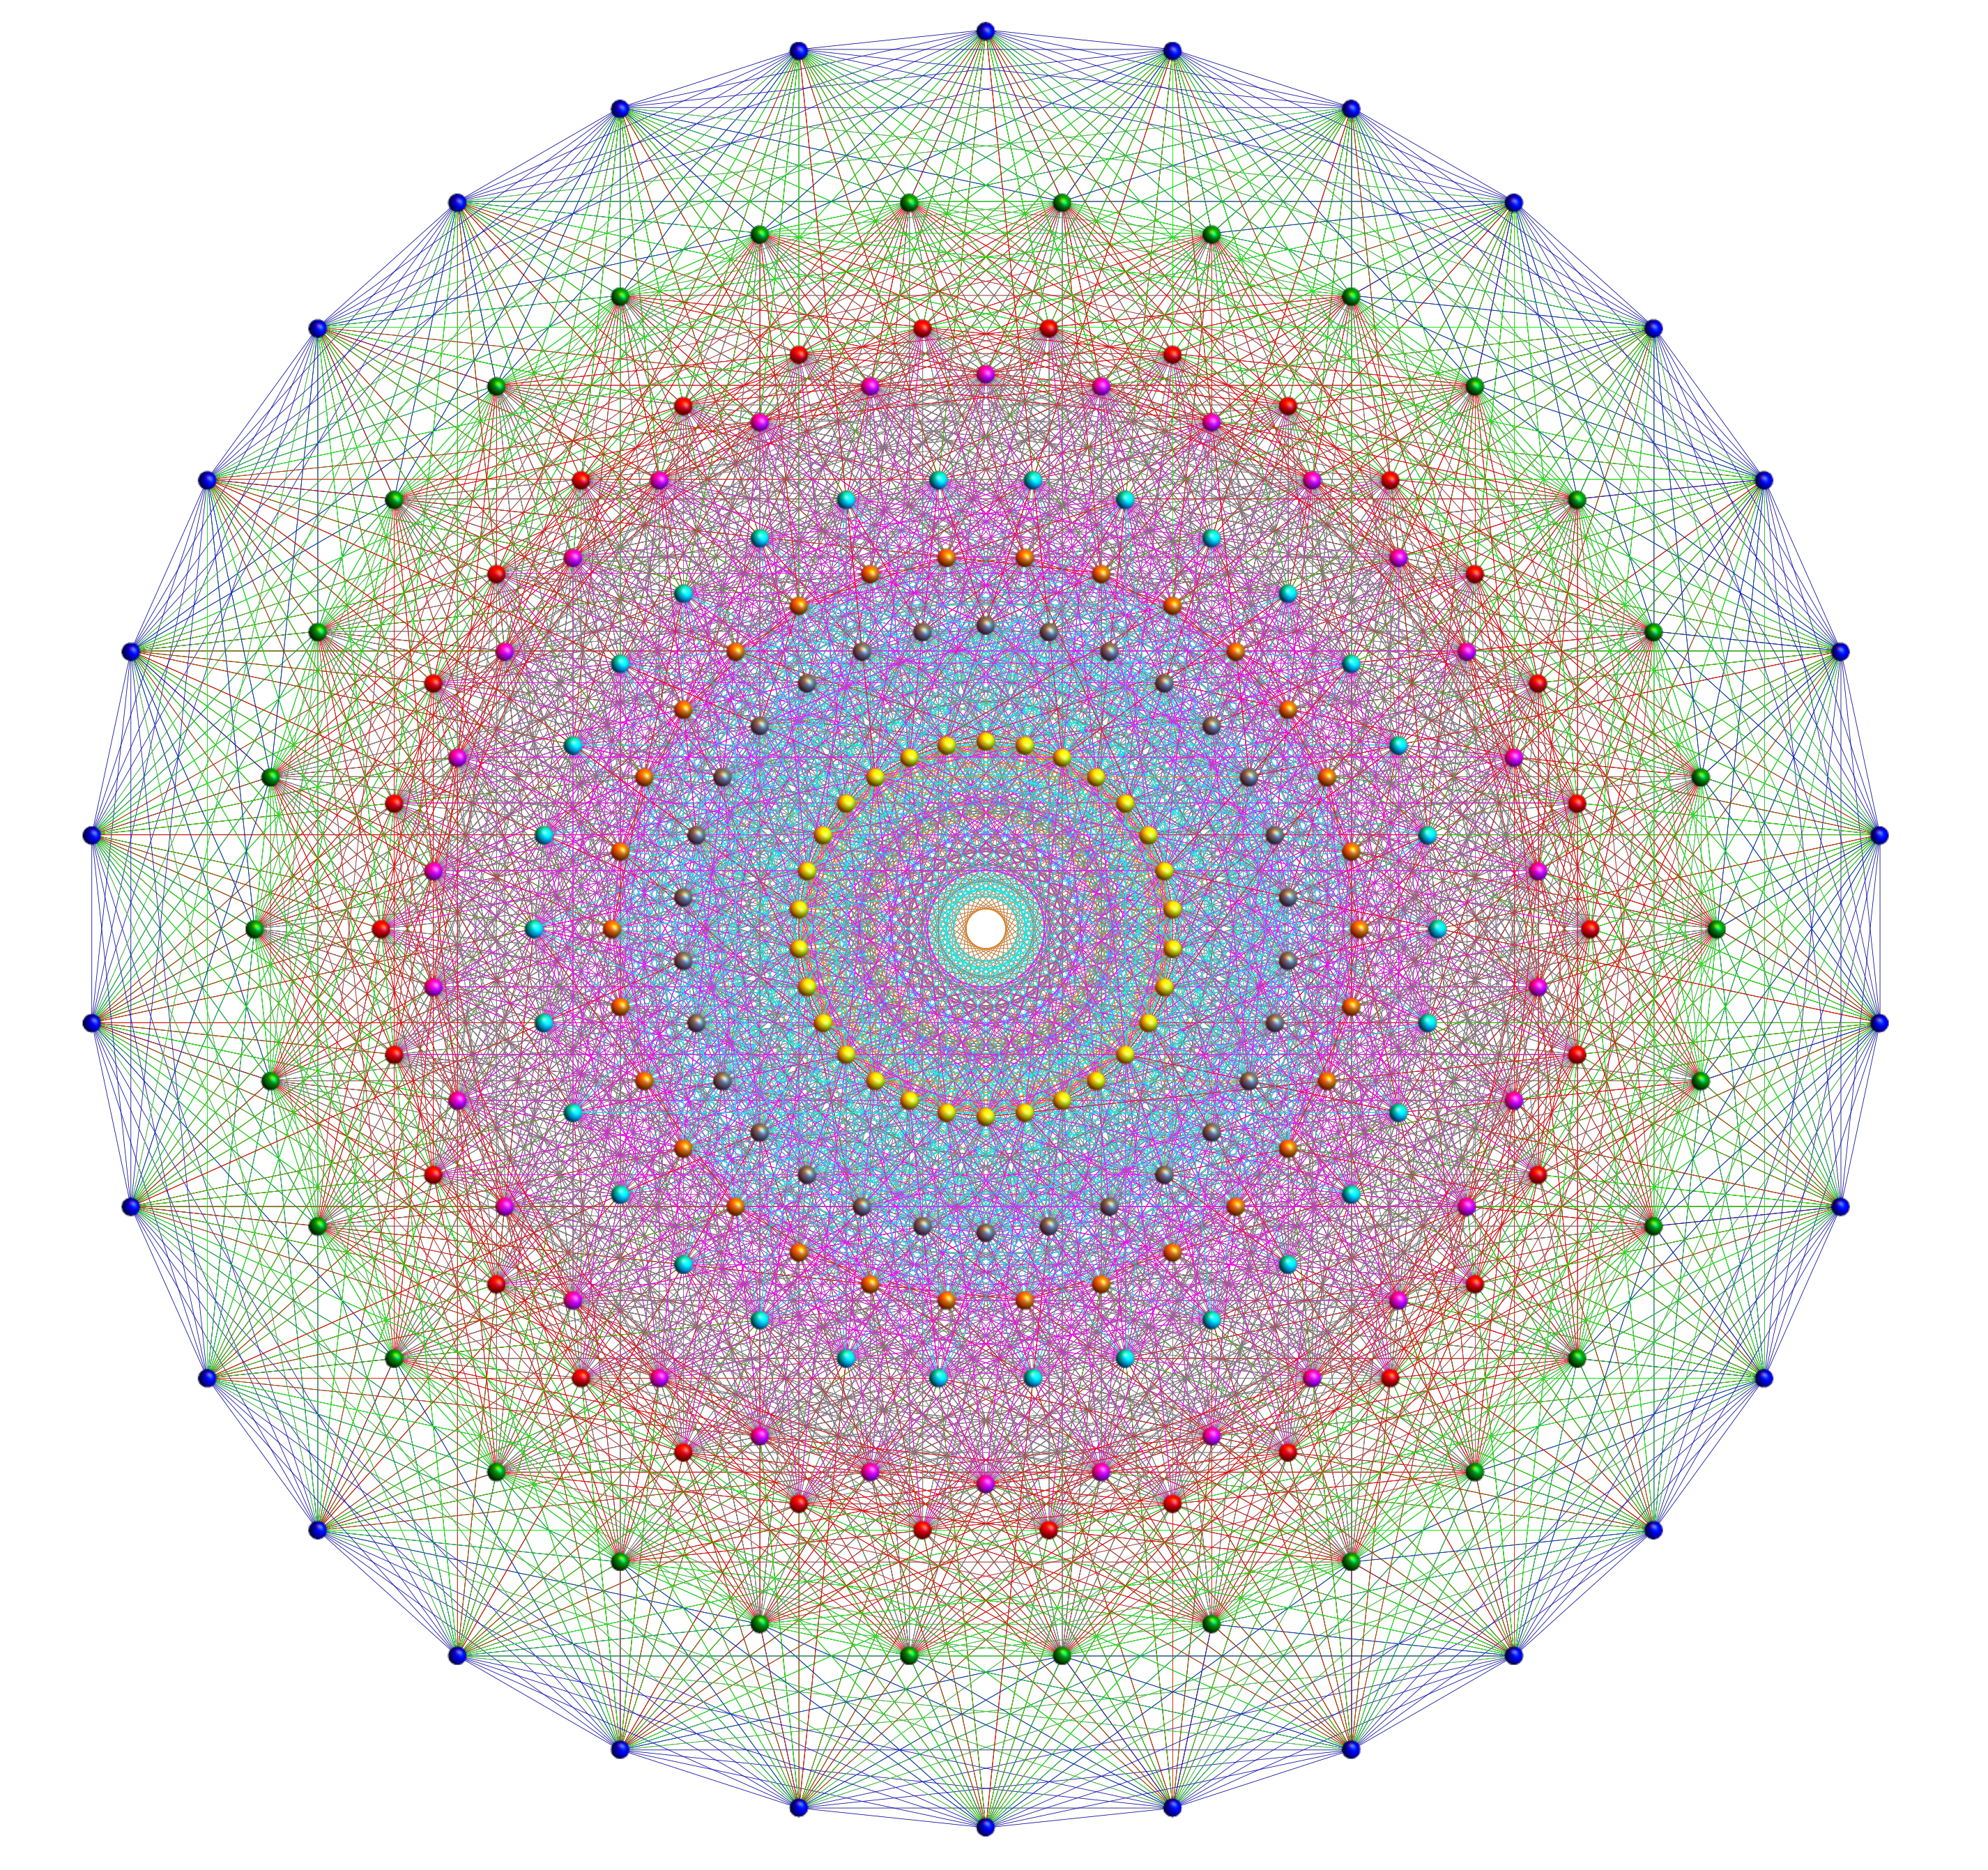
\includegraphics[width=1\columnwidth]{front.jpg}
\end{figure}
\newpage
\tableofcontents 
\newpage
\section{Elettrostatica e conduzione elettrica}
\subsection{Elettrostatica nel vuoto}


Forza della carica $q_1$ su $q_2$, con $\hat{r}_{12}$ diretto da $q_1$ verso $q_2$:
\begin{equation}
	\vec{F}_{12}  = k \frac{q_1q_2}{r^2}\hat{r}_{12} 
\end{equation}
Campo elettrico generato da una carica $Q$ in un certo punto individuato da $\vec{r}$ a partire dalla posizione di $Q$:
\begin{equation}
	\vec{E} = \frac{1}{4\pi \varepsilon_0} \frac{Q}{r^3}\vec{r}
\end{equation}
Il campo generato da una moltitudine di cariche si trova applicando il principio di sovrapposizione. Le linee di forza partono sempre dalle cariche positive e terminano in quelle negative; queste non possono mai incrociarsi altrimenti il vettore campo elettrico non sarebbe ben definito nel punto di incrocio (non sarebbe definito tramite verso, direzione eccetera).

Per una distribuzione continua di carica, volumica per esempio, si ha
\begin{equation}
	\vec{E}(\vec{r}) =\frac{1}{4\pi \varepsilon _0} \int_{\tau } \frac{\rho (\vec{r}')(\vec{r}-\vec{r}')}{\left\lvert \vec{r} - \vec{r}' \right\rvert^3 }d\tau (\vec{r}')
\end{equation}
essendo $dq(\vec{r}) = \rho (\vec{r}) d\tau (\vec{r})$. Per distribuzioni di carica lineare e superficiale si ha, rispettivamente $dq(\vec{r})=\lambda d\ell (\vec{r})$ e $dq(\vec{r}) = \sigma (\vec{r}) dS(\vec{r})$.

\begin{teorema}
	[Teorema di Gauss nel vuoto]
	Il flusso del campo elettrico attraverso una superficie chiusa $S$ \`e 
	\begin{equation}
		\Phi _S(\vec{E}) = \frac{Q_\text{int}}{\varepsilon_0}
	\end{equation}
	Per una distribuzione di carica volumica:
\begin{equation}
	\Phi _S(\vec{E}) = \frac{1}{\varepsilon _0} \int_{\tau } \rho (\vec{r}) d\tau (\vec{r})\equiv \frac{Q_\text{int,tot}}{\varepsilon_0}
\end{equation}	
\end{teorema}
\subsubsection{Teorema della divergenza e I equazione di Maxwell nel vuoto}


\begin{teorema}
	[Teorema della divergenza]
	Sia $\vec{A}$ un campo differenziabile; allora:
	\begin{equation}
		\oint_{S} \vec{E}\cdot d\vec{S}= \int_{\tau } \vec{\nabla }\cdot \vec{E}\ d\tau 
	\end{equation}
\end{teorema}
\noindent Usando il teorema della divergenza, si ottiene la \textbf{prima equazione di Maxwell nel vuoto}:
\begin{equation}
	\vec{\nabla }\cdot \vec{E} = \frac{\rho }{\varepsilon _0}
\end{equation}
\begin{boxenv}[]
\begin{proof}
	Visto che $\Phi_S(\vec{E}) = \frac{1}{\varepsilon _0}\int_{\tau } \rho \ d\tau $, per il teorema della divergenza si ha:
	\[
	\int_{\tau } \vec{\nabla }\cdot \vec{E} = \frac{1}{\varepsilon _0} \int_{\tau } \rho  \ d\tau , \ \forall  \tau 
	\] 
\end{proof}
\end{boxenv}
\noindent Si definisce il potenziale elettrostatico come:
\begin{equation}
	V(r) = \frac{1}{4\pi \varepsilon _0} \frac{Q}{r} +C
\end{equation}
e si ha che
\begin{equation}
	\begin{split}
		&\int_{A} ^B \vec{E}\cdot d\vec{\ell } = \frac{1}{4 \pi \varepsilon _0} \left[ \frac{1}{r_A}-\frac{1}{r_B} \right] \equiv V(A) - V(B)\\
		& \mathcal{L}_A^B (\vec{F}_e) \equiv \int_{A} ^B \vec{F}_e\cdot d\vec{\ell } = q (V_A-V_B)
	\end{split}
\end{equation}
\`E valida la seguente relazione fra campo e potenziale:
\begin{equation}
	\vec{E} = - \vec{\nabla }V
\end{equation}
\begin{boxenv}[]
\begin{proof}
	Per $A,B$ punti vicini fra loro, si ha $-dV = \vec{E}\cdot d\vec{\ell }$, con $d\vec{\ell }= (dx,dy,dz)$. Visto che $V$ \`e una funzione di $x,y,z$, si ha 
	\[
	dV = \frac{\partial V}{\partial x} dx + \frac{\partial V}{\partial y} dy + \frac{\partial V}{\partial z} dz
	\] 
	Riscrivendo l'uguaglianza, si trova:
	\[
	-\frac{\partial V}{\partial x} dx - \frac{\partial V}{\partial y} dy - \frac{\partial V}{\partial z} dz = E_x dx + E_y dy + E_z dz 
	\] 
\end{proof}
\end{boxenv}
\subsubsection{Superfici equipotenziali}


\noindent Le \textbf{superfici equipotenziali} sono tutte e sole quelle la cui direzione $\hat{v}$ \`e tale che 
\[
\frac{\partial V}{\partial \hat{v} }  \equiv \left\lvert \vec{\nabla }V  \right\rvert  \cos \alpha  = 0 \iff\alpha = \frac{\pi}{2} + k\pi
\] 
Dalla relazione $\vec{E} = -\vec{\nabla }V$, si trova che lungo queste superfici, il campo \`e nullo.
\subsubsection{Energia e densit\`a di energia elettrica}


Una carica $q$ posta nel punto $P$ e soggetta ad un potenziale esterno $V(r)$ possiede un'\textbf{energia potenziale elettrostatica} data da:
\begin{equation}
	U = qV(P) = q(V(P) - V(\infty)) =-\int_{\infty} ^P q\vec{E}\cdot d\vec{\ell } =- \mathcal{L}_\infty^P (\vec{F}_e)
\end{equation}
dove si assume $V(\infty) = 0$.

In assenza di campo esterno, l'energia elettrostatica di un sistema composto da $N$ cariche puntiformi \`e l'\textbf{energia di interazione}:
\begin{equation}
	U = \frac{1}{2} \sum_{\substack{i,j\\ i\neq j}}^{N} \frac{q_iq_j}{4\pi \varepsilon _0 r_{ij} } = \frac{1}{2}\sum_{i}^{N} q_i \sum_{\substack{j \\ i\neq j}}^{N} \frac{q_j}{4 \pi \varepsilon _0 r_{ij} } \equiv \frac{1}{2}\sum_{i=1}^{N} q_i V_i
\end{equation}
Per una \textbf{distribuzione continua}, si esegue il passaggio al continuo:
\begin{equation}
	U=\frac{1}{2}\int_{\tau } \rho (x,y,z) V(x,y,z) \ d\tau 
\end{equation}
Questa energia comprende quella di interazione e un'autoenergia.

Un'altra definizione di energia si ha tramite la \textbf{densit\`a di energia} $u$:
\begin{equation}
	U = \int_{\mathbb{R}^3} u(x,y,z) \ d\tau  
\end{equation}
\begin{boxenv}[]
\begin{proof}
	Da $U = \frac{1}{2}\int_{\tau } \rho V \ d\tau $, inserendo la prima equazione di Maxwell per cui $\rho  = \varepsilon _0 (\vec{\nabla }\cdot \vec{E})$, si ha 
	\begin{equation}
		U = \frac{\varepsilon _0}{2} \int_{\tau } V (\vec{\nabla }\cdot \vec{E}) \ d\tau 
	\end{equation}
	Usando $V(\vec{\nabla }\cdot \vec{E}) = \vec{\nabla }\cdot (V\vec{E})+E^2$, si ottengono due integrali; il primo si pu\`o portare ad un integrale di superficie tramite il teorema della divergenza, quindi mandando $\tau \to+\infty$, esso tende a $0$ mentre quello di $E^2$ no in quanto rimane un integrale di volume. Allora il risultato finale \`e proprio quello cercato, con $u = \frac{1}{2}\varepsilon _0 E^2$.
\end{proof}
\end{boxenv}



\subsubsection{Dipolo elettrico}
Due cariche elettriche con vettore distanza $\vec{\delta }$ che punta dalla negativa alla positiva. Momento di dipolo: $\vec{p} = q \vec{\delta }$, con $q$ valore delle cariche.

Per il principio di sovrapposizione, il potenziale generato \`e:
 \begin{equation}
 	V(r) = \frac{\vec{p}\cdot \vec{r}}{4 \pi \varepsilon _0 r^3}
 \end{equation}
In \textbf{coordinate polari} $V(r,\theta ) = \frac{1}{4\pi \varepsilon _0}\frac{p \cos \theta }{r^2}$, per cui usando $\vec{E} = - \vec{\nabla }V$, si ha:
\begin{equation}
	\begin{split}
		&E_r = \frac{1}{4\pi \varepsilon _0} \frac{2 p \cos \theta }{r^3}\\
		&E_\theta  = \frac{1}{4 \pi \varepsilon _0} \frac{p \sin \theta  }{r^3}\\
		& E_\varphi = 0
	\end{split}
\end{equation}
Riscrivendo $r = \sqrt{x^2 + y^2 + z^2} $ e $\vec{p}\cdot \vec{r}= p z$, in coordinate cartesiane, si trova
\begin{equation}
	\vec{E} = \frac{1}{4\pi \varepsilon _0 }\left[ \frac{3(\vec{p}\cdot \vec{r})}{r^5}\vec{r} - \frac{\vec{p}}{r^3} \right] 
\end{equation}
Sotto l'effetto di un generico campo elettrico $\vec{E}$, il dipolo elettrico ha energia:
\begin{equation}
	U = -qV(\vec{r}) + q V(\vec{r}+\vec{\delta }) \simeq q \vec{\nabla }V (\vec{r}) \cdot \vec{\delta } =  -\vec{p}\cdot \vec{E}
\end{equation}
dove $V$ \`e il potenziale generato dal campo elettrico esterno.
\subsubsection{Teorema di Stokes e III equazione di Maxwell}
Per un campo scalare differenziabile $A$, vale la seguente relazione: $\vec{\nabla }\times (\vec{\nabla }A) = 0$.
\begin{teorema}
	[Teorema di Stokes]
	Sia $\vec{v}$ un campo vettoriale, siano $\gamma$ una curva orientata e $S$ la superficie contornata da $\gamma$; allora:
	\begin{equation}
		\oint_{\gamma} \vec{v}\cdot d\vec{\ell } = \int_{S}  (\vec{\nabla }\times \vec{v}) \cdot  dS
	\end{equation}
\end{teorema}
\noindent Da questo, si ottiene la \textbf{III equazione di Maxwell nel vuoto}:
\begin{equation}
	\vec{\nabla }\times \vec{E} = 0
\end{equation}
\begin{boxenv}[]
\begin{proof}
	Visto che il campo elettrico \`e conservativo:
	\[
	\oint_{\gamma} \vec{E}\cdot d\vec{\ell } = 0, \ \forall \gamma
	\] 
	Per il teorema di Stokes deve valere
	\[
	\int_{S}  (\vec{\nabla }\times \vec{E}) \cdot  dS = 0, \ \forall S
	\] 
	da cui si ricava che deve essere l'integrando pari a $0$.
\end{proof}
\end{boxenv}
\subsection{Elettrostatica dei conduttori}
\subsubsection{Reazione di un conduttore ad un campo esterno}


Conduttore $\to$ corpo in cui le cariche sono libere di muoversi. Se posto in campo esterno, non vi \`e campo nel conduttore perch\'e le cariche si dispongono in modo tale da annullarlo (\textbf{all'equilibrio elettrostatico}).

Per Gauss, allora, non vi \`e carica all'interno di un conduttore $\to$ la carica si distribuisce in uno spessore infinitesimo sul bordo del conduttore.

Le linee di forza sono ortogonali alla superficie di ogni conduttore.
\begin{boxenv}[]
\begin{proof}
	Si considera un rettangolo posto tra l'esterno e l'interno del conduttore, con i lati normali alla superficie molto pi\`u corti di quelli tangenziali. La circuitazione del campo elettrico \`e nulla e gli unici contributi sono i lati del rettangolo che si trovano uno nel conduttore, uno nel vuoto. Questo vuol dire che il campo nel vuoto e quello nel conduttore devono essere uguali. Visto che quello nel conduttore deve essere nullo, anche quello all'esterno lo \`e. Questo significa che il campo elettrico subito fuori dal conduttore \`e ortogonale alla superficie del conduttore stesso.
\end{proof}
\end{boxenv}
\noindent Per quanto appena trovato, si conclude che le superfici di un conduttore sono equipotenziali.
\begin{boxenv}[]
	Si pu\`o concludere direttamente dal fatto che il campo \`e ortogonale a tale superficie, da cui anche $\vec{\nabla }V$ lo \`e, visto $\vec{E} = - \vec{\nabla }V$.
\end{boxenv}
\noindent Ogni punto interno del conduttore \`e allo stesso potenziale.
\begin{boxenv}
	\begin{proof}
		Il campo interno \`e nullo, quindi 
		\[
		\int_{A} ^B \vec{E}\cdot d\vec{\ell } = 0 = V_A - V_B \Rightarrow V_A = V_B
		\] 
	\end{proof}
\end{boxenv}
\begin{teorema}
	[Teorema di Coulomb]
	Il campo subito fuori da un conduttore \`e:
	\begin{equation}
		\vec{E} = \frac{\sigma}{\varepsilon _0} \hat{n}
	\end{equation}
	con $\hat{n}$ normale alla superficie del conduttore.
\end{teorema}
\begin{boxenv}[]
\begin{proof}
	Superficie cilindrica con una base (di area $A$) nel conduttore e una nel vuoto $\Rightarrow $ $EA = \frac{\sigma A}{\varepsilon _0}\Rightarrow E = \frac{\sigma}{\varepsilon _0}$. Il campo \`e ortogonale alla superficie.
\end{proof}
\end{boxenv}
\noindent Un conduttore con una cavit\`a interna immerso in campo esterno non presenta cariche al suo interno.
\begin{boxenv}[]
\begin{proof}
	Deve valere $\vec{E}=0$ nel conduttore $\Rightarrow \Phi_S(\vec{E})=0$, quindi per Gauss $q_\text{int} = 0$.
\end{proof}
\end{boxenv}
\noindent Anche sulla superficie della cavit\`a non sono presenti cariche.
\begin{boxenv}[]
\begin{proof}
	Usando lo stesso rettangolino con lati ortogonali alla superficie trascurabili, ed essendo che il campo nel conduttore \`e nullo, anche quello nella cavit\`a \`e nullo. Per il teorema di Coulomb, si ha $\sigma_\text{int}=0$.
\end{proof}
\end{boxenv}
\noindent \textbf{Effetto delle punte} $\to$ parte pi\`u appuntita di un conduttore ha una distribuzione di carica maggiore, quindi esercita un campo elettrico maggiore. 
\begin{boxenv}[]
\begin{proof}
	Si considerano due sfere conduttrici di raggi $R_1, R_2 , \ R_1 \gg R_2$. Collegandole con un filo conduttore, la carica si deve redistribuire in modo che $Q_1 + Q_2 = Q_1' +Q_2'$ e che $\frac{Q_1}{4\pi \varepsilon _0R_1}=V_1 = V_2=\frac{Q_2}{4\pi \varepsilon _0 R_2}$. Risolvendo per $Q_1', Q_2'$, si trova 
	\begin{equation}
		\frac{\sigma _1' }{\sigma_2'}= \frac{R_2}{R_1}
	\end{equation}
	Per $R_1\gg R_2$ si ha $\sigma '_2\gg\sigma '_1$ e per Coulomb $E_1' \ll E_2'$.
\end{proof}
\end{boxenv}

\subsubsection{Capacit\`a elettrica e condensatori}
Dato un conduttore di carica $Q$ con potenziale superficiale $V$, si definisce la sua capacit\`a come
\begin{equation}
	C = \frac{Q}{V}
\end{equation}
\textbf{Condensatore} $\to$ sistema di due conduttori fra i quali c'\`e \textit{induzione completa}\footnote{Per induzione completa, si intende che le linee di forza che partono da un conduttore terminano tutte nell'altro}.

Si \textbf{costruisce} un condensatore sferico. Si prende una sfera di carica $+Q$ e raggio $R_1$ e la si racchiude in una superficie sferica di raggio interno $R_2$ e raggio esterno $R_2'$.

All'equilibrio elettrostatico, non ci deve essere campo elettrico tra $R_2$ e $R_2'$, conclusione che si ottiene usando Gauss con una superficie sferica di raggio $R_2 < r<R_2'$, visto che non vi devono essere cariche interne.

Allora si distribuisce $-Q$ sulla superficie di $R_2$; per lo stesso motivo, $+Q$ si distribuisce sulla superficie di $R_2'$. Collegando la superficie a terra, $R_2'$ si trova a potenziale nullo. 

Il sistema ottenuto \`e complessivamente neutro e vi \`e induzione completa fra le due armature. La differenza di potenziale fra le due armature \`e proporzionale a $Q$:
\begin{equation}
	\Delta V = V_1 - V_2 = \int_{R_1} ^{R_{2} } \vec{E}\cdot d\vec{r}  = \int_{R_1} ^{R_2} \frac{Q}{4\pi \varepsilon _0 r^2}\ dr = \frac{Q}{4\pi \varepsilon _0}\left(\frac{1}{R_1}- \frac{1}{R_{2} }\right) \propto Q 
\end{equation}
Allora si d\`a la definizione di \textbf{capacit\`a di un condensatore} come 
\begin{equation}
	C = \frac{Q}{\Delta V}
\end{equation}
Per il parallelo di due condensatori:
\begin{equation}
	C = C_1 + C_2
\end{equation}
\begin{boxenv}[]
\begin{proof}
	Per il parallelo $\Delta V_1 = \Delta V_2 = \Delta V$ (ddp ai capi di ciascun condensatore), per cui $Q_1=C_1\Delta V$ e $Q_2 = C_2 \Delta V$, da cui $Q = Q_1+Q_2 = \Delta V(C_1+C_2)$.
\end{proof}
\end{boxenv}
Per la serie di due condensatori:
\begin{equation}
	\frac{1}{C} = \frac{1}{C_1}+\frac{1}{C_2}
\end{equation}
\begin{boxenv}
\begin{proof}
	$Q_1=Q_2=Q$, perci\`o la tensione ai capi della serie \`e $\Delta V= \Delta V_1 + \Delta V_2= Q \left(\frac{1}{C_1}+\frac{1}{C_2}\right) $.
\end{proof}
\end{boxenv}
\subsubsection{Pressione elettrostatica}
Pressione dovuta all'interazione di cariche dello stesso segno sulla superficie di un conduttore. Il suo valore \`e dato dalla densit\`a di energia elettrostatica.
\begin{boxenv}[]
\begin{proof}
	Per Coulomb $\vec{E} = \frac{\sigma }{\varepsilon _0}\hat{n}$ fuori dal conduttore. Il campo sentito dalla superficie del conduttore meno un elemento $dS$ \`e:
	\begin{equation}
		\vec{E} = \vec{E}_{(dS)}  + \vec{E}_{(S-dS)} = \frac{\sigma}{\varepsilon _0}\hat{n} \Rightarrow \vec{E}_{(S-dS)} = \frac{\sigma }{2 \varepsilon _0} \hat{n}
	\end{equation}
	La forza su $dS$ \`e
	\begin{equation}
		d\vec{F}=Q_{dS} \vec{E}_{(S-dS)} =\sigma  dS\ \vec{E}_{(S-dS)}  = \sigma dS\ \frac{\sigma }{2\varepsilon _0}\hat{n}=\frac{\sigma ^2}{2\varepsilon _0}dS \hat{n}
	\end{equation}
	Dalla relazione $p = \frac{\left\lvert d\vec{F} \right\rvert }{dS}$, si ottiene proprio $p=u$.
\end{proof}
\end{boxenv}
\subsubsection{Equazioni di Poisson e Laplace e funzioni armoniche}
L'equazione di Poisson \`e:
\begin{equation}
	\nabla ^2 V = -\frac{\rho }{\varepsilon _0}
\end{equation}
\begin{boxenv}[]
\begin{proof}
	Dalla prima equazione di Maxwell $\vec{\nabla }\cdot \vec{E} = \frac{\rho }{\varepsilon _0}$ e da $\vec{E}= - \vec{\nabla }V$, si ottiene l'equazione cercata.
\end{proof}
\end{boxenv}
\noindent La soluzione dell'equazione permette di trovare l'espressione del potenziale generato nello spazio da una distribuzione di carica $\rho $.
\begin{teorema}
	[Teorema di unicit\`a]
Fissata una certa distribuzione di carica $\rho $ e fissate le condizioni al contorno del potenziale date da una superficie $S$ che contorna il volume $\tau $ in cui \`e localizzata $\rho $, l'equazione di Poisson ammette un'unica soluzione per tali condizioni al contorno.
\end{teorema}
\begin{boxenv}[]
\begin{proof}
	Per assurdo $f_1,f_2, \ f_1\neq f_2$ soddisfano $\nabla ^2 f_1 = - \frac{\rho}{\varepsilon _0}$ e $\nabla ^2 f_2 = - \frac{\rho }{\varepsilon _0}$, per cui $f=f_1-f_2$ \`e t.c. $\nabla ^2 f = \nabla ^2 f_1 - \nabla ^2 f_2=0$. Si considera il seguente integrale, che si trova essere nullo tramite il teorema della divergenza per le condizioni al contorno:
	\[
	\int_{\tau } \vec{\nabla }\cdot  (f\vec{\nabla }f) \ d\tau = \int_{S}  (f\vec{\nabla }f) \cdot d\vec{S} = 0
	\] 
	Vale $\vec{\nabla }\cdot  (f\vec{\nabla }f) = f \nabla ^2 f + (\vec{\nabla }f) \cdot (\vec{\nabla }f)=(\vec{\nabla  }f)^2$ perch\'e $\nabla^2 f =0$. Visto che $(\vec{\nabla }f)^2\ge 0$, allora $\vec{\nabla }f=0$ perch\'e l'integrale di partenza sia nullo, quindi $f$ \`e costante. Visto che $f=0$ su $S$ per le condizioni al contorno, allora \`e nulla in tutto $\tau $ e quindi $f_1=f_2$.
\end{proof}
\end{boxenv}
\noindent Nelle regioni di spazio in cui non sono presenti cariche ($\rho =0$), allora si trova l'\textbf{equazione di Laplace}:
\begin{equation}
	\nabla ^2 V = 0
\end{equation}
Le funzioni che la soddisfano sono dette \textbf{armoniche}.
\begin{teorema}
	[Teorema della media]
	Sia $f$ armonica su $\tau $; allora la sua media $\overline{f}$ su una superficie sferica \`e uguale al valore di $f$ nel centro di tale sfera.
\end{teorema}
\subsubsection{Problema fondamentale dell'elettrostatica}

$\to$ Trovare il potenziale generato da un certo numero di conduttori tramite la conoscenza di apposite condizioni al contorno e l'equazione di Laplace $\nabla ^2 V = 0$ applicata alla regione di spazio in cui non sono presenti i conduttori.

Le condizioni al contorno del problema devono stabilire il valore del potenziale all'infinito e sulle superfici dei conduttori.

\begin{itemize}
	\item \textbf{Problema di Dirichlet:} sono noti i $V_i$ sulle superfici dei conduttori e si calcolano le $Q_i$. Soluzione attraverso i punti:
		\begin{itemize}
			\item ricavare $V(\vec{r})$ da $\nabla ^2V = 0$;
			\item ricavare $\vec{E}(\vec{r}) = - \vec{\nabla }V$;
			\item ricavare le densit\`a $\sigma _i(\vec{r})$ da Coulmb;
			\item ricavare le $Q_i$ dalle $\sigma _i$.
		\end{itemize}
	\item \textbf{Problema di Neumann:} sono note le $Q_i$ e si cercano $V_i$. Soluzione attraverso i punti:
		\begin{itemize}
			\item scegliere potenziali arbitrari $V_i^0$ per i conduttori;
			\item risolvere il problema di Dirichlet con $V^0_i$ e trovare $Q_i^0$;
			\item ricavare i coefficienti $C_{ij} $;
			\item impostare i veri valori di $Q_i$ e trovare $V_i$.
		\end{itemize}
\end{itemize}
Per ricavare tutti i $c_{ij} $ si considerano nulli tutti i potenziali eccetto uno, si risolve $\nabla ^2 V=0$ con tali condizioni e si trovano delle cariche $\widetilde{Q}_i$; impostando l'uguaglianza
\[
\widetilde{Q}_i = c_{ij}  V_j 
\] 
si trova una parte dei $c_{ij} $; ripetendo il discorso per tutti i potenziali, si trova la matrice $C$, da cui si ottiene il comportamento del sistema per ogni tipo di condizione al contorno imposta.

\textbf{Metodo delle cariche immagine} $\to$ semplificazione del problema fondamentale che prevede di sostituire il conduttore con cariche immagini la cui sovrapposizione produce un potenziale che rispetti le condizioni al contorno previste dal problema originale. Per l'unicit\`a della soluzione, si \`e risolto il problema di partenza. 

\subsection{Sviluppo in serie di multipoli}

$\to$ Calcolo approssimato per ottenere pi\`u facilmente il potenziale. Si assume che
\begin{itemize}
	\item $\rho \neq 0$ in una regione limitata di spazio $\tau $, con \textit{dimensione caratteristica}\footnote{Grandezza che identifica la dimensione di ordine di grandezza maggiore della regione.} $d$;
	\item $\left\lvert \vec{r} \right\rvert \gg d$.
\end{itemize}
Si considerano volumi infinitesimi di $\tau $, indicati con $d\tau '=dx'dy'dz'$, relativi a $\vec{r}'$. Il contributo infinitesimo di potenziale per $d\tau '$\footnote{Essendo $d\tau '$ molto piccolo, si pensa che il suo potenziale sia come quello di una carica puntiforme, quindi si usa $\vec{r}'$ al denominatore.} \`e $dV(\vec{r}) = \frac{\rho (\vec{r}') d\tau '}{4\pi \varepsilon _0 \left\lvert \vec{r}- \vec{r}' \right\rvert }$. Il potenziale complessivo \`e
\begin{equation}
	V(\vec{r}) = \frac{1}{4\pi \varepsilon _0} \int_{\tau } \frac{\rho (\vec{r}') d\tau '}{\left\lvert \vec{r}- \vec{r}' \right\rvert }\equiv \frac{1}{4\pi \varepsilon _0} \int_{\tau } \rho (\vec{r}') f(\vec{r},\vec{r}') \ d\tau '
\end{equation}
Dalla seconda assunzione, si sviluppa $f$ attorno $\vec{r}' = 0$ (varr\`a $\left\lvert \vec{r} \right\rvert \gg\vec{r}'$):
\begin{boxenv}[]
\begin{equation}
\begin{split}
	f(\vec{r},\vec{r}') \simeq f(\vec{r},0) &+\left(\Eval{\frac{\partial f}{\partial x'} }{\vec{r}' = 0}{}x'+ \Eval{\frac{\partial f}{\partial y'} }{\vec{r}' = 0}{}y'+ \Eval{\frac{\partial f}{\partial z'} }{\vec{r}' = 0}{}z'\right) +\\
				   &+\frac{1}{2}\Eval{\frac{\partial ^2f}{\partial x'^2} }{\vec{r}' = 0}{}x'^2+\frac{1}{2}\Eval{\frac{\partial ^2f}{\partial y'^2} }{\vec{r}' = 0}{}y'^2+\frac{1}{2}\Eval{\frac{\partial ^2f}{\partial z'^2} }{\vec{r}' = 0}{}z'^2+\\
				   &+\Eval{\frac{\partial ^2 f}{\partial x'\partial y'} }{\vec{r}'=0}{}x'y'+\Eval{\frac{\partial ^2 f}{\partial y'\partial z'} }{\vec{r}'=0}{}y'z'+\Eval{\frac{\partial ^2 f}{\partial x'\partial z'} }{\vec{r}'=0}{}x'z'
\end{split}
\end{equation}
\noindent L'ordine 0 si indica con $f^{(0)} $, l'ordine 1 con $f^{(1)} $ e il 2 con $f^{(2)} $.
\end{boxenv}
\noindent Il potenziale sar\`a la somma dei potenziali ai vari gradi di approssimazione. 

\subsubsection{Termine di monopolo}
Si considera $f=f^{(0)} $. Allora
\begin{boxenv}[]
\begin{equation}
	V^{(0)} (\vec{r}) = \frac{1}{4 \pi \varepsilon _0 r}\int_{\tau } \rho (\vec{r}') d\tau '= \frac{q}{4\pi\varepsilon _0r}
\end{equation}
\end{boxenv}
\noindent La carica $q$ \`e detta \textbf{momento di monopolo}.

\subsubsection{Termine di dipolo}

Si considera $f^{(1)} $ con
\begin{equation}
	\begin{split}
		&\Eval{\frac{\partial f}{\partial x'} }{\vec{r}'=0}{} = \frac{x}{r^3}; \ \Eval{\frac{\partial f}{\partial y'} }{\vec{r}'=0}{} = \frac{y}{r^3}; \ \Eval{\frac{\partial f}{\partial z'} }{\vec{r}'=0}{} = \frac{z}{r^3}\\
		&\Rightarrow f^{(1)} = \frac{x'x}{r^3} + \frac{y'y}{r^3} + \frac{z'z}{r^3} = \frac{\vec{r}\cdot \vec{r}' }{r^3}
	\end{split}
\end{equation}
Il potenziale \`e
\begin{equation}
	\begin{split}
		V^{(1)} (\vec{r}) &= \frac{1}{4 \pi \varepsilon _0} \int_{\tau } \frac{\vec{r}\cdot \vec{r}'}{r^3}\rho (\vec{r}') \ d\tau '= \frac{1}{4\pi \varepsilon _0 r^3}\vec{r} \int_{\tau } \vec{r}' \rho (\vec{r}') \ d\tau '\\
				  &\equiv \frac{\vec{r}\cdot \vec{p}}{4\pi \varepsilon _0r^3}
	\end{split}
\end{equation}
Integrale $\vec{p}$ noto come \textbf{momento di dipolo}. Per due cariche puntiformi, ha l'espressione gi\`a trovata.
\begin{boxenv}[]
\begin{proof}
	Per due cariche $+q$, $-q$ a distanza $\vec{d}$ (da negativa a positiva) vale $\rho (\vec{r}') = -q \delta (\vec{r}' - \vec{r}_1) + q \delta (\vec{r}'-\vec{r}_2)$\footnote{$\vec{r}_1$ raggio vettore per $-q$, $\vec{r}_2$ per $+q$ | vale $\vec{r}_2 = \vec{r}_1 +\vec{d}$}. Allora:
	\begin{equation}
		\begin{split}
			\vec{p}&= -q \int_{\tau } \vec{r}' \delta (\vec{r}' - \vec{r}_1) \ d\tau ' + q \int_{\tau } \vec{r}' \delta (\vec{r}' - \vec{r}_1 - \vec{d}) \ d\tau ' \\
			&= -q \vec{r}_1 + q (\vec{r}_1 + \vec{d}) = q \vec{d} \\
		\end{split}
	\end{equation}
\end{proof}
\end{boxenv}
\subsubsection{Termine di quadrupolo}
Vale
\begin{equation}
	\begin{split}
		&\Eval{\frac{\partial ^2f}{\partial x'_ix'_j} }{\vec{r}' =0}{} = \frac{3 x_i x_j}{r^5} - \frac{\delta _{ij} }{r^3}\\
		&\begin{split}
			\Rightarrow f^{(2)} &= \frac{1}{2}\Eval{\frac{\partial ^2f}{\partial x'_ix'_j} }{\vec{r}' =0}{} x'_i x'_j =\frac{1}{2r^5} \sum_{i,j}^{} (3x_{i} x_j - r^2 \delta _{ij} ) x_i' x_j'\\
					    &=\frac{1}{6r^5}\left[ \sum_{i,j}^{} (9x_ix_jx_i'x_j') - 3r^2r'^2 \right] \\
					    &=\frac{1}{6r^5}\sum_{i,j}^{} \left(3x_i x_j - \delta _{ij} r^2\right) \left(3x_i'x_j' - \delta _{ij} r'^2\right) 
		\end{split}
	\end{split}
\end{equation}
Si dimostra l'ultima uguaglianza.
\begin{boxenv}[]
\begin{proof}
	\begin{equation}
		\begin{split}
			\sum_{i,j}^{} \left(3x_i x_j - \delta _{ij} r^2\right) &\left(3x_i'x_j' - \delta _{ij} r'^2\right) =\\
									       &= \sum_{i,j}^{} 9x_ix_jx_i'x_j' - 3r'^2 r^2 - 3r^2 r'^2 + \underbracket{\sum_{i}^{} r^2 r'^2}_{=3r^2 r'^2} \\
			&=\sum_{i,j}^{} (9x_ix_jx_i'x_j') - 3 r'^2 r^2
		\end{split}
	\end{equation}
\end{proof}
\end{boxenv}
\noindent Il potenziale di quadrupolo \`e
\begin{equation}
	\begin{split}
		V^{(2)} (\vec{r}) &= \frac{1}{4\pi \varepsilon _0}\frac{1}{6r^5} \sum_{i,j}^{} \left(3x_ix_j - \delta _{ij} r^2\right) \underbracket{\int_{\tau } \left[ 3x_i'x_j' - \delta _{ij} r'^2 \right] \rho (\vec{r}') \ d\tau '}_{\equiv Q_{ij} } \\
				  &=\frac{1}{4\pi \varepsilon _0}\frac{1}{6r^5} \sum_{i,j}^{} \left(3x_ix_j - \delta _{ij} r^2\right)Q_{ij} 
	\end{split}
\end{equation}
$Q_{ij} \to $ \textbf{momento di quadrupolo} ed \`e un tensore del secondo ordine, simmetrico e con traccia nulla. 
\subsection{Elettrostatica nei dielettrici}
Dielettrici $\to$ isolante polarizzabile da campo esterno. Si assumeranno omogenei e isotropi\footnote{Rispettivamente invarianza delle caratteristiche del materiale per traslazioni e per rotazioni.}.

Il campo sentito dal singolo atomo o molecola $i$-esima \`e
\begin{equation}
	\vec{E}_{l,i} = \vec{E}+\sum_{j\neq i}^{} \vec{E}_j
\end{equation}
con $\vec{E}$ campo esterno e $\vec{E}_j$ campo generato dalla molecola $j$-esima per polarizzazione. La somma dei campi degli altri atomi o molecole sottintende una media su $d\tau $ e $dt$ per eliminare le fluttuazioni.
\subsubsection{Effetti sulla capacit\`a}
Condensatore piano con armature separate da dielettrico. Si verifica una diminuzione della tensione fra le armature dovuta al dielettrico, quindi cambia il campo elettrico e cambia la capacit\`a del condensatore. \textbf{Costante dielettrica relativa}:
\begin{equation}
	\varepsilon _r \equiv \frac{\Delta V}{\Delta V'} >1
\end{equation}
Campo elettrico precedente $E=\Delta V / d$ implica che il nuovo \`e:
\begin{equation}
	E' = \frac{\Delta V}{\varepsilon _r d}
\end{equation}
La nuova capacit\`a \`e:
\begin{equation}
	C' = \varepsilon _r C = \varepsilon _r \varepsilon _0 \frac{S}{d} \equiv \varepsilon  \frac{S}{d}
\end{equation}
dove $\varepsilon $ \textbf{costante dielettrica assoluta del materiale} e $\varepsilon >\varepsilon _0$. 

In presenza di campo esterno, il dielettrico si polarizza o per deformazione o per orientamento.
\subsubsection{Polarizzazione per deformazione}

Atomo immerso in campo locale (diretto verso il basso) $\vec{E}_l \to$ il nucleo si sposta verso il basso di $\vec{r}$. Spostato dal centro, il nucleo percepisce il campo $\vec{E}_{at} $ generato dalla nube elettronica. Modellando l'atomo come una sfera di raggio $R$:
\begin{equation}
	|\rho| = \frac{Ze}{\frac{4}{3}\pi R^3} \Rightarrow \vec{E}_{at} = -\frac{\rho  r}{3 \varepsilon _0} \hat{r}
\end{equation}
Per trovare $r$ si deve avere il nucleo in equilibrio, quindi si sfrutta la relazione $\left\lvert \vec{E}_{at}  \right\rvert = \left\lvert \vec{E}_l \right\rvert$:
\begin{equation}
	r=\frac{3\varepsilon_0}{|\rho| }\left\lvert \vec{E}_l \right\rvert 
\end{equation}
Il momento di dipolo indotto \`e:
\begin{equation}
	\vec{p}=Ze \vec{r}= Ze \frac{3\varepsilon _0}{|\rho |}\vec{E}_l = 4\pi \varepsilon _0 R^3 \vec{E}_l\equiv \alpha _D \vec{E}_l
\end{equation}
$\alpha _D$ \`e la \textbf{polarizzabilit\`a elettronica}, di espressione generale data da $\alpha _D = 3 \varepsilon _0 \mathcal{V}$ ($\mathcal{V} $ volume della figura, sfera in questo caso).

\subsubsection{Polarizzazione per orientamento}

$\to$ Molecole con atomi che hanno momento di dipolo $\vec{p}_0$ permanente polarizzano per campo locale $\vec{E}_l$. Inizialmente ($E_l = 0$), gli atomi hanno momenti orientati casualmente $\Rightarrow $ la molecola ha $\left\langle p \right\rangle=0$.

L'energia di ciascun atomo \`e $U = - \vec{p}_0 \cdot \vec{E}_l = - p_0E_l \cos \theta \Rightarrow $ dipolo si allineerà con il campo locale per minimizzare energia.

A equilibrio termodinamico, la molecola sar\`a a temperatura $T\to$ perturbazione da energia minima. La propensione degli atomi ad allinearsi col campo locale \`e $\frac{U}{\kappa _B T}$ e si usa la distribuzione di Boltzmann 
\begin{equation}
	W(U) = A e^{-\frac{U}{\kappa _B T}} 
\end{equation}
per indicare la distribuzione probabilistica dell'allineamento dei dipoli dovuta ad agitazione termica.

Energia indipendente da angolo azimutale $\varphi \Rightarrow $ configurazioni a stessa energia rappresentate da una circonferenza. Ci si pu\`o spostare di $d\theta $ e trovare la stessa energia, per cui si individua regione $d\Omega_0$ a uguale energia che descrive anello $d\Omega $ in cui si ha stessa configurazione energetica. Allora $W(U) d\Omega $ \`e la probabilit\`a che il dipolo sia orientato in $d\Omega$. Vale che
\begin{equation}
	\begin{split}
		&d\Omega_0 = \frac{dS}{r^2}=\sin \theta  d\theta  d\varphi, \ dS = r d\theta  r \sin \theta  d\varphi \\
		&\Rightarrow d\Omega = 2 \pi \sin \theta  d\theta \\
		&\Rightarrow dW \equiv W(U) d\Omega = Ae^{- \frac{U}{\kappa _B T}}  d\Omega =A\exp \left(\frac{p_0 E_l \cos \theta }{\kappa _B T}\right) 2\pi\sin \theta  d\theta  
	\end{split}
\end{equation}
Considerando $U \ll \kappa _B T$, si sviluppa l'esponenziale attorno a $0$ fino al primo ordine, quindi
\begin{equation}
	dW \simeq 2\pi A \left(1+ \frac{p_0 E_l \cos \theta }{\kappa _B T}\right) \equiv \frac{1}{2}\left[ 1+ \frac{p_0 E_l \cos \theta }{\kappa _B T} \right] \sin \theta  d\theta 
\end{equation}
Questa \`e una densit\`a probabilit\`a, quindi deve fare $1$ se integrata da $\theta =0$ a $\theta =\pi$; in questo modo si trova $A = \frac{1}{4 \pi}$.

Ora si pu\`o calcolare $\left\langle p_z \right\rangle$\footnote{Non si ha motivo di supporre che il momento di dipolo della molecola si distribuir\`a in una direzione diversa da quella del campo esterno.} come
\begin{equation}
	\begin{split}
		\left\langle p_z \right\rangle &= \int p_z\ dW = \int p_0\cos \theta\  dW = \int_{0} ^\pi p_0 \cos \theta  \frac{1}{2}\left[ 1+ \frac{p_0 E_l \cos \theta }{\kappa _B T} \right] \sin \theta  \ d \theta \\
					       &= \frac{p_0^2 E_l }{3\kappa _B T}
	\end{split}
\end{equation}
Si risolve prendendo $x=\cos \theta $. Inoltre si chiama $\alpha _0 \equiv \frac{p_0^2}{3\kappa _B T}$ \textbf{polarizzabilit\`a per orientamento}. 

La polarizzazione per deformazione \`e sempre presente, ma quando \`e presente anche quella per orientamento, si considera $\alpha  = \alpha _D + \alpha_0 \simeq \alpha _0$.

\subsubsection{Vettore di polarizzazione elettrica}
Porzione $\Delta \tau $ di volume di un dielettrico; si definisce:
\begin{equation}
	\vec{P} = \lim_{\Delta \tau  \to 0} \frac{1}{\Delta \tau }\sum_{i}^{} \vec{p}_i
\end{equation}
Si riscrive come:
\begin{equation}
	\begin{split}
		&\left\langle \vec{p} \right\rangle = \frac{1}{\Delta N} \sum_{i}^{} \vec{p}_i \Rightarrow \sum_{i}^{} \vec{p}_i = \Delta N \left\langle \vec{p} \right\rangle\\
		&\Rightarrow \vec{P} = \lim_{\Delta \tau\to 0} \frac{\Delta N}{\Delta \tau } \left\langle \vec{p} \right\rangle\equiv n \left\langle \vec{p} \right\rangle
	\end{split}
\end{equation}
con $\Delta N$ numero di dipoli in $\Delta \tau $ e $n$ densit\`a di dipoli in $\Delta \tau $.
\subsubsection{Cariche di polarizzazione}
Dielettrico con $\vec{P}$ generico. Porzione di volume del dielettrico $d\tau '$ in posizione $\vec{r}'$. Si calcola potenziale nel punto $A$ in $\vec{r}$. In $d\tau '$, si ha $d\vec{p} = \vec{P}d\tau '$; il contributo della porzione \`e
\begin{equation}
	dV(\vec{r}) = \frac{1}{4\pi \varepsilon _0} \frac{d\vec{p}\cdot (\vec{r}-\vec{r}')}{\left\lvert \vec{r}-\vec{r}' \right\rvert^3}
\end{equation}
Per tutto il dielettrico:
\begin{equation}
	V(\vec{r}) = \frac{1}{4\pi \varepsilon _0} \int_{\tau }  \frac{\vec{P}\cdot (\vec{r}-\vec{r}')}{\left\lvert \vec{r}-\vec{r}' \right\rvert ^3}\ d\tau '
\end{equation}
Dato che
\begin{equation}
	\begin{split}
		&\vec{\nabla }' \overset{\text{def}}{=} \left(\frac{\partial }{\partial x'} , \frac{\partial }{\partial y'}, \frac{\partial }{\partial z'} \right) \\
		&\Rightarrow \vec{\nabla }' \frac{1}{\left\lvert \vec{r}-\vec{r}' \right\rvert } = \frac{\vec{r}-\vec{r}'}{\left\lvert \vec{r}-\vec{r}' \right\rvert ^3} = - \vec{\nabla } \frac{1}{\left\lvert \vec{r}-\vec{r}' \right\rvert}\\
		&\Rightarrow V(\vec{r}) = \frac{1}{4\pi \varepsilon _0}\int_{\tau } \vec{P}(\vec{r}') \cdot \vec{\nabla }' \frac{1}{\left\lvert \vec{r}- \vec{r}'\right\rvert}\ d\tau 
	\end{split}
\end{equation}
Usando $\vec{\nabla }\cdot (f\vec{g}) = \vec{\nabla }f \cdot \vec{g} + f\vec{\nabla }\cdot \vec{g}$, con $f = \frac{1}{\left\lvert \vec{r}- \vec{r}'\right\rvert }$ e il teorema della divergenza, si ha:
\begin{equation}
	V(\vec{r}) = \frac{1}{4 \pi \varepsilon _0}\int_{S} \frac{\vec{P}(\vec{r'})\cdot \hat{n}}{\left\lvert \vec{r}-\vec{r}' \right\rvert } \ dS + \frac{1}{4\pi \varepsilon _0} \int_{\tau } \frac{- \vec{\nabla }'\cdot \vec{P}(\vec{r}')}{\left\lvert \vec{r}-\vec{r}' \right\rvert }\ d\tau '
\end{equation}
Per il teorema di unicit\`a:
\begin{equation}
	\begin{cases}
		\sigma _P = \vec{P}\cdot \hat{n}\\
		\rho _P = - \vec{\nabla }'\cdot \vec{P}
	\end{cases}
\end{equation}
con $\hat{n}$ normale alla superficie che contorna il dielettrico. Per $\vec{P}$ uniforme, $\rho _P = 0$.

\subsubsection{Suscettivit\`a elettrica}

Per \textbf{materiali rarefatti} $\vec{E}_l \simeq \vec{E}\Rightarrow \vec{P} = n \left\langle \vec{p} \right\rangle$, con $\left\langle \vec{p} \right\rangle= \alpha \vec{E}_l = \alpha \vec{E}$. Quindi
\begin{equation}
	\vec{P} =  n \alpha  \vec{E} = \varepsilon _0 \chi  \vec{E}
\end{equation}
con $\chi = \frac{n\alpha }{\varepsilon _0}$ suscettivit\`a elettrica.

Per \textbf{liquidi non polari} (solo deformazione) $\vec{E} = \vec{E}_l + \vec{E}_i\Rightarrow \vec{E}_l = \vec{E} + \frac{\vec{P}}{3\varepsilon _0}$, immaginando che ogni molecola sia una sfera polarizzata. Allora:
\begin{equation}
	\vec{P} = n\alpha \vec{E}_l = n \alpha  \left(\vec{E}+ \frac{\vec{P}}{3\varepsilon _0}\right) \Rightarrow \vec{P}= \frac{n\alpha }{1-\frac{n\alpha }{3\varepsilon _0}}\vec{E} \equiv \varepsilon _0 \chi \vec{E}
\end{equation}
Visto che\footnote{Non ancora dimostrato.} $\chi = \varepsilon _r -1$:
\begin{equation}
	\frac{n\alpha }{\varepsilon _0 \left(1- \frac{n\alpha }{3\varepsilon _0}\right) } = \varepsilon _r - 1 \Rightarrow \alpha = \frac{3\varepsilon _0}{n}\frac{\varepsilon _r-1}{\varepsilon _r+2}
\end{equation}
nota come \textbf{relazione di Clausius-Mossotti}. Questa funziona bene per solidi a struttura cubica, ma non per gli altri.
\subsubsection{Equazioni di Maxwell per dielettrici}

Continua a valere $\vec{\nabla }\times \vec{E}=0$ perch\'e $\vec{E}$ \`e conservativo. La prima va modificata per tenere conto delle cariche di polarizzazione. Vale:
\begin{equation}
	\begin{split}
		&\vec{\nabla }\cdot \vec{E} = \frac{\rho  + \rho _P}{\varepsilon _0} = \frac{\rho  - \vec{\nabla }\cdot \vec{P}}{\varepsilon _0} \Rightarrow  \varepsilon _0 \vec{\nabla }\cdot \vec{E} = \rho  - \vec{\nabla }\cdot \vec{P}\\
		&\Rightarrow \vec{\nabla }\cdot \vec{D}= \rho 
	\end{split}
\end{equation}
con $\vec{D} = \varepsilon _0 \vec{E}+\vec{P}$ \textbf{vettore di spostamento elettrico}. Per \textbf{dielettrici perfetti, omogenei e isotropi}:
\begin{equation}
	\begin{split}
		&\vec{P} = \varepsilon _0 \chi \vec{E} \\
		&\Rightarrow  \vec{D} = \varepsilon _0 (1+\chi )\vec{E} = \varepsilon _0 \varepsilon _r \vec{E}\equiv \varepsilon \vec{E}\\
		&\Rightarrow \vec{ P} = \frac{\varepsilon _r -1}{\varepsilon _r}\vec{D}
	\end{split}
\end{equation}
Dalla prima equazione di Maxwell corretta, se $\vec{E}_0$ \`e il campo nel vuoto, si ricava che:
\begin{equation}
	\vec{E} = \frac{\vec{E}_0}{\varepsilon _r}
\end{equation}
\subsubsection{Teoremi di Gauss e Coulomb}

Dalla prima, si ottiene una versione modificata del \textbf{teorema di Gauss}:
\begin{equation}
	\Phi_S (\vec{D}) = \int_{S} \vec{D}\cdot d\vec{S} = Q_\text{int}
\end{equation}
\begin{boxenv}[]
\begin{proof}
Integrando sul volume del dielettrico:
\begin{equation}
	\int_{S} \vec{D} \cdot d\vec{S}=\int_{\tau } \vec{\nabla }\cdot \vec{D} \ d\tau = \int_{\tau } \rho \ d\tau  = Q_\text{int}
\end{equation}
\end{proof}
\end{boxenv}
\noindent Applicando Gauss all'interfaccia fra dielettrico e un conduttore, si ha il \textbf{teorema di Coulomb}:
\begin{equation}
\vec{D} = \sigma \hat{n}
\end{equation}
\subsubsection{Relazione tra $\chi $ e $\varepsilon _r$}
Condensatore con armature con distribuzione $\sigma $ e $-\sigma $; alle estremit\`a del dielettrico fra le armature si distribuisce rispettivamente $-\sigma _P$ e $+ \sigma _P$. Il campo \`e $\vec{E} = \frac{\vec{E}_0}{\varepsilon _r}$.

Usando Gauss su una superficie cilindrica con basi parallele ad un'armatura tale da comprendere all'interno $+\sigma$ e $-\sigma _P$:
\begin{equation}
	\Phi_S(\vec{E}) = AE = \frac{Q_\text{int}}{\varepsilon _0} = \frac{(\sigma - \sigma _P)A}{\varepsilon _0} \Rightarrow E = \frac{\sigma -\sigma _P}{\varepsilon _0}
\end{equation}
Usando $\sigma _P = \vec{P}\cdot \hat{n}\Rightarrow \left\lvert \sigma _P \right\rvert = \left\lvert \vec{P} \right\rvert $ e $\vec{P} = \varepsilon _0 \chi \vec{E}$ (in questo caso, il coseno \`e $+1$ o $-1$):
\begin{equation}
	E = \frac{\sigma -\varepsilon _0 \chi E}{\varepsilon _0} = \frac{\varepsilon _0 E_0 - \varepsilon _0 \chi E}{\varepsilon _0}= E_0 - \chi E \Rightarrow E = \frac{E_0}{1+ \chi }
\end{equation}
Allora $\varepsilon _r = 1+\chi $.

\subsubsection{Legge di rifrazione del campo elettrico}
Interfaccia fra due dielettrici con $\varepsilon _1 = \varepsilon _0 \varepsilon _{r,1}, \ \varepsilon _2 = \varepsilon _0 \varepsilon _{r,2}  $ in assenza di cariche libere. Per la componente ortogonale, si considera un cilindro con $\sqrt{A} \gg dh$; applicando Gauss al cilindro $S$ e usando $\hat{n}_1 = - \hat{n}_2$:
\begin{equation}
	0=\oint_{S} \varepsilon \vec{E}\cdot d\vec{S} \equiv A\left[ \vec{D}_1 \cdot \hat{n}_1 + \vec{D}_2 \cdot \hat{n}_2 \right] = D_{1\perp} - D_{2 \perp} \Rightarrow D_{1\perp}  = D_{2\perp} 
\end{equation}
Per la componente parallela, si prende un rettangolo con $h\ll \ell $ (altezza e lato parallelo). $\vec{E}$ conservativo, quindi, usando $d\vec{l}_1 = -d\vec{l}_2$:
\begin{equation}
	0=\oint_{L} \vec{E}\cdot d\vec{l} = \vec{E}_2 \cdot d\vec{l}_2 + \vec{E}_1 \cdot d\vec{l}_1 \Rightarrow E_{1 | |} = E_{2 | |}  
\end{equation}
Unendo i due risultati:
\begin{equation}
	\begin{cases}
		 \varepsilon _{r,1}  E_{1}\cos\theta _1  = \varepsilon _{r,2} E_{2}\cos\theta _2 \\
		 E_1 \sin \theta _1 =  E_2\sin \theta _2 
	\end{cases} \Rightarrow \frac{\varepsilon _{r,1} }{\varepsilon _{r,2} } = \frac{\tan \theta _1}{\tan\theta _2}
\end{equation}
\subsubsection{Energia elettrostatica per dielettrici}
Vale ancora 
\begin{equation}
	U = \frac{1}{2}\int_{\tau }  \rho  V \ d\tau 
\end{equation}
dove $\rho $ \`e la densit\`a di cariche libere e $V$ \`e il potenziale dovuto sia a quelle libere che quelle di polarizzazione.

Per procedimenti analoghi al caso di una distribuzione continua di carica, usando $\vec{\nabla }\cdot \vec{D} = \rho $, si arriva alla conclusione che
\begin{equation}
	U = \frac{1}{2}\int \vec{D} \cdot  \vec{E} \ d\tau = \int \frac{1}{2}\varepsilon  |\vec{E} |^2 \ d\tau 
\end{equation}
dove l'integrale \`e su tutto lo spazio, con $u\equiv \frac{1}{2}\varepsilon  E^2$ densit\`a di energia.


\subsection{Conduzione elettrica}
\subsubsection{Corrente elettrica}
$\to$Moto ordinato delle cariche positive in un conduttore quando sottoposto ad un campo esterno. \`E:
\begin{equation}
	I = \frac{dQ}{dt}
\end{equation}
Se $\Delta V$ costante, $I$ \`e stazionaria.
\subsubsection{Modello di Drude}

La densit\`a di elettroni liberi per unit\`a di volume \`e:
\begin{equation}
	n = \frac{Z \rho _m N_A}{A}
\end{equation}
dove $A$ \`e la massa atomica, $Z$ \`e il numero di elettroni di valenza del conduttore, $\rho _m$ la densit\`a del materiale conduttore, $A$ \`e la massa atomica e $N_A$ il numero di Avogadro.

Il modello di Drude afferma che gli elettroni urtano gli ioni; dopo l'urto gli elettroni prendono una velocit\`a con direzione casuale e modulo dipendente dalla temperatura nel punto dell'urto pari a $v_T$.

Il tempo medio fra due collisioni $\tau  = \frac{\Delta \ell }{v_T}$, con $\Delta \ell $ cammino libero medio\footnote{Indica lo spostamento medio fra un urto e l'altro di un elettrone.}; un buon valore per $\Delta \ell $ \`e la distanza fra due ioni. In presenza di campo esterno $\vec{E}$, $\vec{a} = \frac{- e\vec{E}}{m_e}$; prendendo come velocit\`a iniziale quella termica, fra un urto e l'altro, la legge oraria dell'elettrone \`e:
\begin{equation}
	\begin{split}
		&\vec{v}(t)  =  \vec{v}_T  - e \frac{\vec{E}}{m_e} t\\
		&\Rightarrow \left\langle \vec{v}(t) \right\rangle  =  \left\langle \vec{v}_T  \right\rangle - e \frac{\vec{E}}{m_e} \tau  \equiv - e \frac{\vec{E}}{m_e} \tau 
	\end{split}
\end{equation}
perch\'e in media $\left\langle v_T \right\rangle=0$ visto che dopo un urto, ha direzione casuale. Per il teorema di equipartizione
\begin{equation}
	\frac{1}{2}m\left\langle v^2 \right\rangle= \frac{3}{2}\kappa _BT\Rightarrow v_T = \sqrt{3 \kappa _B T / m} 
\end{equation}
quindi inserendo $\tau  = \frac{\Delta \ell }{v_T}$:
\begin{equation}
	\vec{v}_d = \frac{-e \Delta \ell }{\sqrt{3 \kappa _B T m } }\vec{E}
\end{equation}
\`e la \textbf{velocit\`a di deriva}. In genere $v_D \ll v_T$.

\subsubsection{Densit\`a e intensit\`a di corrente elettrica}

Si considera un cilindro all'interno del quale scorrono cariche. Data $d\vec{S}$ al suo interno, se $n =$ densit\`a di portatori di carica liberi di carica $q$ e $\vec{v}_D$ campo di velocit\`a di deriva, la superficie \`e attraversata da un quantitativo di carica
\begin{equation}
	dq_{dS}  = nq \vec{v}_D \cdot d\vec{S}dt\Rightarrow dq_{S} = dt \int_{S} nq\vec{v}_D \cdot d\vec{S} 
\end{equation}
ogni intervallo temporale $dt$. Definendo $\vec{j} = nq \vec{v}_D$:
\begin{equation}
	I_S = \int_{S} \vec{j}\cdot d\vec{S}\hspace{2mm} \text{ (attraverso } \vec{S}\text{)}
\end{equation}

\subsubsection{Conducibilit\`a e resistivit\`a}

Essendo $\vec{v}_D = k \vec{E}$\footnote{Qui si \`e chiamato $k = \frac{-e \Delta l}{\sqrt{3\kappa _B T m } }$.}, vale $\vec{j}= nqk \vec{E}$, dove $\sigma \equiv nq k$ ed \`e detta \textbf{conducibilit\`a elettrica}. \textbf{Resistivit\`a} definita come $\rho = 1 / \sigma $, per cui $\vec{E} = \rho  \vec{j}$. Per modello di Drude $\rho  \propto 1 / \tau \propto 1 / \sqrt{T} $, ma in realt\`a si osserva una dipendenza lineare approssimata come
\begin{equation}
	\rho  - \rho_0 = \rho_0 \alpha  (T-T_0), \ \rho_0 = \rho (T_0)
\end{equation}
con $\alpha $ \textbf{coefficiente di temperatura}. 

\subsubsection{Equazione di continuit\`a della corrente}

$S$ superficie immaginaria qualsiasi (fissa) che circonda $\tau $. All'interno, c'\`e una carica $Q(t)$ che fuoriesce dalla superficie. La variazione \`e:
\begin{equation}
	-dQ = \int_{S} \vec{j}\cdot d\vec{S}dt \Rightarrow \frac{d Q}{d t} = - \int_{S} \vec{j}\cdot d\vec{S}
\end{equation}
Visto che $Q = \int_{\tau } \rho  \ d\tau $, si ha
\begin{equation}
	\int_{\tau } \frac{\partial \rho }{\partial t} \ d\tau = - \int_{S} \vec{j}\cdot d\vec{S}
\end{equation}
Usando il teorema della divergenza sul secondo membro e visto che l'uguaglianza deve valere $\forall \tau $, allora:
\begin{equation}
	\frac{\partial \rho }{\partial t}  + \vec{\nabla }\cdot \vec{j} = 0
\end{equation}
nota come \textbf{equazione di continuit\`a della corrente}.

\subsubsection{Correnti stazionarie}

Le correnti stazionarie si riferiscono al caso in cui $\vec{\nabla }\cdot  \vec{j} = 0$, quindi, localmente, non vi sono variazioni nella distribuzione delle cariche\footnote{Perch\'e $\vec{\nabla }\cdot \vec{j} = 0 \Rightarrow  \frac{\partial \rho }{\partial t}  = 0 $.}, di fatto il flusso complessivo della densit\`a di corrente \`e nullo a indicare che tante sono le cariche che entrano, tante sono quelle che escono, il che porta ad avere complessivamente una corrente costante nel tempo.

\subsubsection{Leggi di Kirchhoff}
Per correnti stazionarie, valgono:
\begin{itemize}
	\item $\sum_{i}^{} I_i = 0$, con $i$ ramo attraverso cui scorre $I_i$;
	\item $\sum_{i}^{} \Delta V_i = 0$.
\end{itemize}
La prima si giustifica dalla stazionariet\`a; la seconda dal fatto che correnti stazionarie generano campi elettrostatici\footnote{Questo perch\'e $\frac{\partial \rho }{\partial t} = 0 $, quindi si hanno campi elettrostatici generati da distribuzioni di cariche che rimangono costanti nel tempo.} per cui $\vec{\nabla }\times \vec{E}=0$, quindi la circuitazione di $\vec{E}$ su tutto il circuito \`e nulla.

Valgono anche per correnti \textbf{lentamente variabili} purch\'e il tempo di variazione sia molto maggiore di quello che impiega la corrente a percorrere il circuito; in questo caso, si possono usare le leggi di Kirchhoff istante per istante.

\subsubsection{Legge di Ohm}

Per certi materiali (\textbf{ohmici}) vale $\Delta V = R I$, con $R$ \textbf{resistenza}. Questa \`e data da:
\begin{equation}
	R = \frac{\ell }{S} \rho 
\end{equation}
con $\ell $ lunghezza del materiale, $S$ superficie e $\rho $ resistivit\`a elettrica (che dipende dalla temperatura). Si definisce \textbf{conducibilit\`a elettrica} $\sigma  = \frac{1}{\rho }$. Per \textbf{materiali ohmici}\footnote{Vale anche per materiali non ohmici, ma $\rho $ non \`e uniforme e dipende da $\left\lvert \vec{E} \right\rvert $.} vale:
\begin{equation}
	\vec{E} = \rho  \vec{j} \Rightarrow \vec{j} = \sigma  \vec{E}
\end{equation}
\begin{boxenv}[]
\begin{proof}
	$R= \rho  \frac{\ell }{S}\Rightarrow \Delta V = \rho  \frac{\ell }{S}I\Rightarrow E \equiv \frac{\Delta V}{\ell }= \rho \frac{I}{S}\equiv \rho  j$.  
\end{proof}
\end{boxenv}
\noindent Per resistenze in \textbf{serie} vale $R_\text{eq} = R_1+R_2$, mentre per il \textbf{parallelo} vale $\frac{1}{R_\text{eq} }= \frac{1}{R_1}+\frac{1}{R_2}$.

\noindent \textbf{NOTA:} per conduttori non-ohmici, vale $\Delta V=RI$, ma $R\equiv f(\Delta V)$. 
\subsubsection{Correnti radiali}

Si considera lo scorrimento di corrente, in verso radiale, attraverso un cilindro cavo conduttore che ha raggio interno $r_A$ e raggio esterno $r_B$ e altezza $h$.

Si considera un guscio cilindrico di raggio $r$, spessore $dr$ e altezza $h$; allora $S = 2 \pi r h$ mentre $\ell = dr$ perci\`o $dR = \rho  \frac{dr}{2\pi r h}$. La resistenza complessiva \`e:
\begin{equation}
	R = \int_{r_A} ^{r_B} \rho  \frac{dr}{2\pi r h} = \frac{\rho }{2 \pi h}\ln \frac{r_B}{r_A} 
\end{equation}

\subsubsection{Dielettrici non perfetti}

$\to$ Dielettrici in cui pu\`o scorrere corrente. Ponendo questo tra le armature di un condensatore di forma generica, usando una superficie $S$ anch'essa generica fra le due armature:
\begin{equation}
	\int_{S} \vec{E}\cdot d\vec{S} = \int_{S} \rho  \vec{j}\cdot d\vec{S} = \rho I
\end{equation}
Contemporaneamente:
\begin{equation}
	Q = \int_{S} \vec{D}\cdot d\vec{S}\Rightarrow \int_{S} \vec{E}\cdot d\vec{S} = \frac{Q}{\varepsilon } \Rightarrow \rho I = \frac{Q}{\varepsilon }
\end{equation}
Se il dielettrico \`e \textbf{ohmico} $\Rightarrow I = \frac{\Delta V}{R}$; per il condensatore $Q = C\Delta V$, per cui:
\begin{equation}
	RC = \rho \varepsilon 
\end{equation}
\subsubsection{Effetto Joule}
L'energia generata dal campo elettrico per il moto delle cariche viene dissipata sotto forma di energia termica per effetto Joule. La potenza \`e $W = \frac{dL}{dt}$ con $dL = dq (V_A-V_B)$ e $dq = I dt$ per cui
\begin{equation}
	W = I \Delta V = RI^2 = \frac{\Delta V^2}{R}
\end{equation}
Questo si ha perch\'e il conduttore oppone una certa resistenza al passaggio di cariche.

La \textbf{forma locale} dell'effetto Joule \`e:
\begin{equation}
	\frac{dL}{d\tau dt} = \vec{E}\cdot \vec{j}
\end{equation}
\begin{boxenv}[]
\begin{proof}
	$dL = dq (V_A -V_B)$ con $dq$ cariche in volume $d\tau $ e $dq = nq d\tau $ per $n$ densit\`a di cariche. Si prende $d\tau $ di lunghezza $d\vec{\ell }=\vec{v}_D dt$. Allora
	\begin{equation}
		dL = nqd\tau  \vec{E}\cdot \vec{v}_D dt = \vec{E}\cdot (nq\vec{v}_D) d\tau dt = \vec{E}\cdot \vec{j}d\tau dt
	\end{equation}
\end{proof}
\end{boxenv}
\noindent Questa rappresenta la potenza dissipata per unit\`a di volume.
\subsubsection{Forza elettromotrice}

$\to$ Nome assegnato al lavoro del campo elettrico non conservativo che permette la chiusura di un circuito elettrico.

Un \textbf{generatore di fem} ha un accumulo di cariche positive sull'\textbf{anodo} e di cariche negative sul \textbf{catodo}; permette di trasportare cariche dall'anodo al catodo e ricominciare il processo. Per fare ci\`o e mantenere una differenza di potenziale costante nel circuito bisogna mantenere gli accumuli di carica costanti, quindi \`e necessario far passare cariche positive dal catodo all'anodo; allora c'\`e un campo non conservativo $\vec{E}_e$ (\textbf{campo elettromotore}) che punta da $ C\to A$ che permette questo moto e si oppone al campo elettrostatico $\vec{E}_s$ generato dall'accumulo di cariche di segno opposto tra anodo e catodo.

La forza elettromotrice \`e definita come:
\begin{equation}
	f = \int_{C} ^A \vec{E}_e \cdot d\vec{l}
\end{equation}
dove $C$ sta per catodo e $A$ sta per anodo. Il campo elettrico totale che interessa il circuito \`e dato da $\vec{E}_\text{tot} = \vec{E}_s + \vec{E}_e$; allora
\begin{equation}
	\oint_{l} \vec{E}_\text{tot}\cdot d\vec{l} = \oint_{l} \vec{E}_S \cdot d\vec{l} + \oint_{l} \vec{E}_e \cdot d\vec{l} = \int_{C} ^A \vec{E}_e\cdot d\vec{l} 
\end{equation}
Allora
\begin{equation}
	f\equiv\oint_{l} \vec{E}\cdot d\vec{l}
\end{equation}

\subsubsection{Fem per generatori ideali e reali}

Circuito aperto (solo generatore) e condizioni stazionarie $\Rightarrow \left\lvert \vec{E}_e \right\rvert = \left\lvert \vec{E}_s \right\rvert$ quindi:\footnote{Ancora $A$ indica l'anodo e $C$ il catodo.}
\begin{equation}
	f = -\int_{C} ^A \vec{E}_s \cdot d\vec{l} =V(A) - V(C)
\end{equation}
A circuito chiuso, se generatore \textbf{ideale} sarebbe costante $f = V(A) - V(C)$; in realt\`a 
\begin{equation}
	V(A) - V(C) = f - rI
\end{equation}
con $r$ resistenza interna del generatore. Andamento $\Delta V$ all'aumentare di $I$ \`e lineare fino a una certa $I_\text{max}$, dopo di che crolla a picco.
\subsubsection{Potenza del generatore}
Data da $W_g = \frac{d L_g}{d t} $, dove $dL_g = dq f = fI dt$, quindi:
\begin{equation}
	W_g = fI
\end{equation}
Una parte di questa \`e dissipata dalla resistenza interna ($W_d$), l'altra trasferita al carico ai capi del generatore:
\begin{equation}
	\begin{split}
		&W_g = I (V_A -V_B) + W_d \Rightarrow  fI = I (V_A -V_B) + W_d\\
		&\Rightarrow f = V_A -V_B + \frac{W_d}{I}\\
		&\Rightarrow W_d = rI^2
	\end{split}
\end{equation}
Per i \textbf{carichi ohmici}, la potenza viene dissipata in calore. Per \textbf{carichi non-ohmici}, la potenza viene trasformata in altre forme di energia. 

\subsubsection{Campi contro-elettromotori}

Per carichi non-ohmici (come bobine o condensatori) si sviluppano dei campi contro-elettromotori $\vec{E}_c$ che si oppongono alla variazione dell'intensit\`a di corrente. La \textbf{forza contro-elettromotrice} associata \`e:
\begin{equation}
	f_C = \int_{A} ^B \vec{E}_c \cdot d\vec{l}
\end{equation}
se la corrente scorre da $B$ verso $A$.
\subsubsection{Legge di Ohm generalizzata}

Si considera una componente ohmica (i cui terminali sono $A$ e $B$) attraversata da campi elettromotori e contro-elettromotori:
\begin{equation}
	\begin{split}
		&\vec{E} = \vec{E}_s + \vec{E}_e + \vec{E}_c = \rho \vec{j}\\
		&\Rightarrow (V_A - V_B) + \sum_{i}^{} f_{e,i} + \sum_{i}^{} f_{c,i} = \int_{A} ^B \rho \vec{j}\cdot d\vec{l} 
	\end{split}
\end{equation}
dove si \`e calcolato il lavoro di tutti i campi da $A$ a $B$ terminali della componente. Il membro di destra \`e:
\begin{equation}
	\int_{A} ^B \rho \vec{j}\cdot d\vec{l} \equiv \int_{A} ^B \rho  j dl = \int_{A} ^B \rho  \frac{I}{S} dl = I \int_{A} ^B \rho  \frac{dl}{S} = I R_{AB} 
\end{equation}
dove si assume $\vec{j}| | \vec{S}$ e $\sqrt{S} \ll l$ (lunghezza tubo di flusso) per avere $\vec{j}$ omogeneo. Per una maglia, vale la \textbf{II legge di Kirchhoff generalizzata} ottenuta tramite circuitazione:
\begin{equation}
\sum_{i}^{} f_{e,i} + \sum_{i}^{} f_{c,i} = \sum_{i}^{} R_i I_i
\end{equation}
\subsubsection{Conduttori attraversati da corrente}

Si considerano correnti stazionarie. Vale $\vec{E}_\text{int}\neq 0$ perch\'e cariche nel conduttore sono in moto. Per questo, la superficie non \`e pi\`u equipotenziale e, quindi, il campo elettrico esterno non \`e pi\`u ortogonale alla superficie del conduttore.

\begin{enumerate}
	\item All'interno del conduttore \textbf{non ci possono essere accumuli di carica}. Visto che $\vec{\nabla }\cdot \vec{E}_\text{int} = \frac{\rho_c }{\varepsilon _0}$ e che $\vec{E}_\text{int} = \rho  \vec{j}$, allora $\vec{\nabla }\cdot  (\rho \vec{j}) = \frac{\rho _c}{\varepsilon _0}$. Per conduttori ohmici $\Rightarrow \varepsilon _0 \rho \vec{\nabla }\cdot \vec{j} = \rho _c = 0$ (cond. stazionarie $\vec{\nabla }\cdot \vec{j}=0$), quindi non vi possono essere accumuli di carica interni al conduttore ohmico. Utilizzando la legge di Ohm locale, si arriva alla stessa conclusione anche per materiali non-ohmici. Questa conclusione si pu\`o anche vedere come l'assenza di uno squilibrio di carica: in un conduttore attraversato da corrente, non sono presenti squilibri di carica negativi o positivi.

	\item La densit\`a $\vec{j}$ \`e \textbf{sempre parallela alla superficie} del conduttore. Per vederlo, si usa Gauss con un cilindro di altezza trascurabile rispetto all'area delle basi. Versore $\hat{n}$ indica la normale alla superficie, $\hat{\theta }$ indica quella parallela. Visto che $\vec{\nabla }\cdot \vec{j}=0\Rightarrow \Phi(\vec{j}) = 0$. Il flusso attraverso la superficie superiore \`e nullo perch\'e \`e nel vuoto, quello attraverso le superfici trascurabili \`e nullo, quindi il flusso attraverso base inferiore \`e anch'esso nullo. Quindi la componente di $\vec{j}$ normale al conduttore \`e nulla, quindi $\vec{j} ||\hat{\theta }$:
		\begin{equation}
			\vec{j} = j \hat{\theta } = \frac{I}{S}\hat{\theta }
		\end{equation}
	\item Il campo interno \`e $\vec{E}_\text{int}= \rho  \vec{j} = \rho \frac{I}{S}\hat{\theta }$. Si \`e visto che la componente parallela del campo si conserva nel passaggio da conduttore ad altro mezzo, quindi $E_{| |, \text{ext}} = \rho j$.
	\item La componente normale \`e $E_{\perp, \text{ext}} = \frac{\sigma_c}{\varepsilon _0}$ per via delle cariche disposte sulla superficie del conduttore. Si trova usando Gauss con la superficie al punto (2) e serve a mantenere il campo interno parallelo al conduttore.
\end{enumerate}
\subsubsection{Scarica di un condensatore}
A $t=0$ condensatore carico con $Q_0$. La carica lascia il condensatore e si dissipa nella resistenza. 
\begin{equation}
	\begin{split}
		&\begin{cases}
		V(t) = RI(t) \\
		V(t) = \frac{Q(t)}{C} 
	\end{cases}\Rightarrow RI(t) = - R \frac{d Q}{d t} = \frac{Q(t)}{C}\\
		&\Rightarrow Q(t) = Q_0 e^{ - t / \tau }\\
		&\Rightarrow I(t) = \frac{d Q}{d t}  = \frac{Q_0}{\tau }e^{-t / \tau } \equiv I_0 e^{-t / \tau } 
	\end{split}
\end{equation}
La potenza dissipata dal processo \`e $W = RI(t)^2$, allora
\begin{equation}
	U  = \int_{0} ^{+\infty} RI_0e^{-t / \tau } \ dt  = \frac{Q_0^2}{2C}
\end{equation}
Questa \`e l'energia immagazzinata dal condensatore inizialmente e poi totalmente dissipata dalla resistenza.
\subsubsection{Carica di un condensatore}
Generatore di fem $\equiv f$ e $V(t)$ tensione ai capi di $C\Rightarrow f- V(t) = RI(t)$:
\begin{equation}
	\begin{split}
		&R \frac{d Q}{d t}  + \frac{Q}{C} = f\\
		&\Rightarrow Q(t) = Ae^{-t / \tau } + fC \equiv fC(1- e^{- t / \tau } )
	\end{split}
\end{equation}
con $A=-fC$ perch\'e $Q(0) = 0$. Da questo si trova
\begin{equation}
	\begin{cases}
		\displaystyle V(t) = \frac{Q}{C} = f(1- e^{-t / \tau }) \\
		\\
		\displaystyle I(t) = \frac{d Q}{d t} = \frac{f}{R} e^{-t / \tau } 
	\end{cases}
\end{equation}
La potenza erogata dal generatore \`e $W = If$, quindi:
\begin{equation}
	U = \int_{0} ^{+\infty} fI \ dt = f \int_{0} ^{+\infty} \frac{f}{R}e^{-t / \tau } \ dt = \frac{f^2}{R}\tau  = f^2 C
\end{equation}
L'energia immagazzinata dal condensatore \`e $U = \frac{1}{2}CV^2 \to \frac{1}{2}Cf^2$ per $t\to +\infty$; l'altra met\`a di energia rimanente erogata \`e consumata per effetto Joule attraverso $R$.

\newpage

\section{Magnetismo}

\subsection{Magnetismo nel vuoto}

\subsubsection{Forza di Lorentz}


Un circuito percorso da corrente stazionaria presenta un tratto $dl$ mobile attaccato a due molle e lo si immerge in un campo magnetico. Sperimentalmente, la forza sentita dal tratto $d\vec{l}$ \`e:
\begin{equation}
	d\vec{F} = Id \vec{l}\times \vec{B}
\end{equation}
Si considera un volume $d\tau  = dl S$ nel quale scorre una corrente $I$; allora $I d\vec{l} = jS d\vec{l} \equiv \vec{j}d\tau = nq \vec{v}_d d\tau $, con $n=\frac{dN}{d\tau }$ cio\`e la densit\`a di portatori di carica nel cilindro. Si ha $Id\vec{l} = dN q\vec{v}_d$
\begin{equation}
	\Rightarrow d\vec{F} = dN q\vec{v}_d \times \vec{B}
\end{equation}
Una singola carica percepisce la \textbf{forza di Lorentz}:
\begin{equation}
	\vec{F} = q\vec{v}\times \vec{B}
\end{equation}
La sua forma pi\`u generale comprende anche la forza relativa al campo elettrico:
\begin{equation}
	\vec{F} = q\vec{v} \times \vec{B}  + q \vec{E}
\end{equation}
Escludendo il campo elettrico:
\begin{itemize}
	\item se $\vec{v}= 0 \Rightarrow \vec{F} = 0$ (cariche ferme, niente forza);
	\item si ha $\vec{F}\perp \vec{v}\Rightarrow \mathcal{L}(\vec{F}) = 0$ cio\`e la forza magnetica non compie lavoro;
	\item $\vec{F}$ non compie lavoro, quindi modifica la direzione di $\vec{v}$.
\end{itemize}
\subsubsection{Momento di una spira rigida}

La forza netta che agisce su una spira in campo $\vec{B}$ uniforme \`e nulla:
\begin{equation}
	\vec{F} = \oint_{L} I d\vec{l} \times \vec{B} =0 
\end{equation}
Il momento, invece, \`e dato da:
\begin{equation}
	\vec{\Gamma} = I\vec{S} \times \vec{B}\equiv \vec{m}\times \vec{B}
\end{equation}
con $\vec{S}$ orientata da vedere la corrente in senso anti-orario e $\vec{m}$ momento magnetico della spira.
\begin{boxenv}[]
\begin{proof}
	Spira rettangolare per esempio, ma valido per forma generica. La somma delle forze agenti \`e $\vec{F} = 0$ come visto. Tutta via, se $\vec{B}$ forma un angolo $\theta $ con la normale alla spira $\hat{n}$, una coppia di forze fa momento. Siano $a$ i lati lungo cui la forza fa momento e $b$ gli altri:
	\begin{equation}
		\Gamma_i = IaB \frac{b}{2}\sin\theta 
	\end{equation}
	con $\frac{b}{2}\sin \theta $ braccio della forza. Allora:
	\begin{equation}
\Gamma_\text{tot} = IaB b \sin \theta  = IB S \sin \theta = I \vec{S}\times \vec{B} 
	\end{equation}
\end{proof}
\end{boxenv}
\begin{teorema}
	[Teorema di equivalenza di Amp\`ere]
	Una spira percorsa da corrente stazionaria con momento $\vec{m}$ \`e equivalente ad un dipolo magnetico con stesso momento $\vec{m}$.
\end{teorema}
\subsubsection{Sollecitazioni meccaniche su circuiti}

Principio dei lavori virtuali su un circuito $\to$ spostamento $d\vec{s}$ a velocit\`a trascurabile. Su un tratto $d\vec{l}$ di circuito agisce $d\vec{F} = Id\vec{l}\times \vec{B}$. Deve esistere\footnote{Per il teorema delle forze vive, se $\Delta K = 0$, allora anche il lavoro compiuto dalle forze agenti sul sistema deve esserlo.} $d\vec{f} = -d\vec{F}$ per frenare il moto; $dL = dU$ lavoro di $d\vec{f}$\footnote{Gli integrali sono riferiti a tutta la spira e sono rispetto a $d\vec{l}$ contenuto nella forza esterna e in $d\vec{F}$.}:
\begin{equation}
	dL = \oint_l d\vec{f}\cdot d\vec{s}  = - \oint_{l} d\vec{F}\cdot d\vec{s} = - I \oint_{l}  (d\vec{l}\times \vec{B}) \cdot d\vec{s} =  I \oint_{l}  (d\vec{l}\times d\vec{s}) \cdot \vec{B}
\end{equation}
usando $(d\vec{l}\times \vec{B}) \cdot d\vec{s} = - (d\vec{l}\times d\vec{s}) \cdot \vec{B}$. Se $\hat{n}$ normale al piano dato da $d\vec{s}$ e $d\vec{l}\Rightarrow d\vec{l}\times d\vec{s} = dl ds \sin \theta  \hat{n}\equiv d\vec{S}$ superficie parallelogramma. Allora 
\begin{equation}
	dL = I \int_{d\Sigma} d\vec{S}\cdot \vec{B} \equiv I \Phi _{d\Sigma}(\vec{B})  
\end{equation}
con $d\Sigma$ superficie laterale dello spostamento del circuito. Se $\Sigma$ \`e l'area racchiusa dal circuito iniziale e $\Sigma'$ da quello finale, usando che $\vec{\nabla }\cdot \vec{B} = 0$, vale $\Phi^\text{out} _\Sigma(\vec{B})+\Phi^\text{out} _{\Sigma'}(\vec{B}) + \Phi^\text{out} _{d\Sigma} (\vec{B}) = 0$. Essendo $\Phi_\Sigma(\vec{B})^\text{in} = - \Phi_{\Sigma}^\text{out} (\vec{B})$:
\begin{equation}
	\begin{split}
		&\Phi^\text{in} _\Sigma(\vec{B})=\Phi^\text{out} _{\Sigma'}(\vec{B}) + \Phi^\text{out} _{d\Sigma} (\vec{B})\Rightarrow d\Phi(\vec{B}) = 	\Phi^\text{out} _{\Sigma'}(\vec{B})-\Phi^\text{in} _\Sigma(\vec{B}) = - \Phi_{d\Sigma}^{\text{out}} (\vec{B}) \\
		&\Rightarrow dU = I\Phi_{d\Sigma}(\vec{B}) = - I d\Phi (\vec{B})\\
		&\Rightarrow U = - I \Phi(\vec{B})
	\end{split}
\end{equation}
\subsubsection{Legge di Biot-Savart}

Tratto di filo $d\vec{l}'$ in posizione $\vec{r}'$; il campo magnetico generato nel punto $P$ in posizione $\vec{r}$ \`e:
\begin{equation}
	d\vec{B}_0 (\vec{r})= \frac{\mu_0}{4 \pi} I \frac{d\vec{l}' \times (\vec{r}-\vec{r}')}{\left\lvert \vec{r}-\vec{r}' \right\rvert ^3}
\end{equation}
Il contributo di tutto il circuito \`e:
\begin{equation}
	\vec{B} (\vec{r}) = \frac{\mu_0}{4\pi}I \oint_{l'} \frac{d\vec{l}' \times (\vec{r}-\vec{r}')}{\left\lvert \vec{r}-\vec{r}' \right\rvert^3 }
\end{equation}
Questo vale per un circuito \textbf{filiforme}; per un circuito \textbf{spesso} si ha
\begin{equation}
	\begin{split}
		&I = \int_{S'}\vec{j}(\vec{r}') \cdot d\vec{S}\\
		&\Rightarrow\vec{B}(\vec{r}) = \frac{\mu _0}{4 \pi }\int_{l'} \int_{S'} \left[ \vec{j}(\vec{r}')\cdot d\vec{S}' \right] \frac{d\vec{l}'\times (\vec{r}-\vec{r}')}{\left\lvert \vec{r}-\vec{r}' \right\rvert ^3}
	\end{split}
\end{equation}
con $\vec{S}'$ superficie nel tubo di flusso. Visto che $\vec{j}\cdot d\vec{S}' = JdS'_n$ con $dS'_n = dS' \cos \alpha $\footnote{Angolo fra $\vec{j}$ e $\vec{dS}'$.}, allora $jdS'_n d\vec{l}' = \vec{j}dS'_n dl' = \vec{j}d\tau '$:
\begin{equation}
	\vec{B}(\vec{r}) = \frac{\mu _0}{4\pi} \int_{\tau '} \frac{\vec{j}(\vec{r}') \times (\vec{r}-\vec{r}')}{\left\lvert \vec{r}-\vec{r}' \right\rvert^3 }d\tau '
\end{equation}
\subsubsection{II equazione di Maxwell}

Spira non filiforme $\to$ legge di Biot-Savart non filiforme; il termine $\Delta \vec{r} / \left\lvert \Delta \vec{r} \right\rvert ^3 = -\vec{\nabla } \frac{1}{\Delta r}$. Si usa la relazione $\vec{\nabla }\times (f \vec{v}) = f\vec{\nabla }\times \vec{v} + \vec{\nabla }f \times \vec{v}$ e si ottiene un termine contenente $\vec{\nabla }\times \vec{j}(\vec{r}') =0$ perch\'e $\vec{j}$ dipende da $\vec{r}' $, non da $\vec{r}$. Allora:
\begin{equation}
	\vec{B}(\vec{r}) = \frac{\mu_0}{4 \pi }\int_{\tau '} \vec{\nabla }\times \frac{\vec{j}(\vec{r}')}{\Delta r}d\tau ' = \vec{\nabla }\times \left[ \frac{\mu_0}{4\pi}\int_{\tau '} \frac{\vec{j}(\vec{r}')}{\Delta r }d\tau ' \right] 
\end{equation}
visto che rotore e integrale agiscono su coordinate diverse. Si definisce \textbf{potenziale vettore} 
\begin{equation}
	\begin{split}
		&\vec{A} = \frac{\mu_0}{4 \pi }\int_{\tau '} \frac{\vec{j}(\vec{r}') }{\left\lvert \vec{r}-\vec{r}' \right\rvert }d\tau ' \text{ (non filiformi}) \\
		&\vec{A} = \frac{\mu_0}{4 \pi }I\int_{l '} \frac{d\vec{l}' }{\left\lvert \vec{r}-\vec{r}' \right\rvert }  \text{ (filiformi}) 
	\end{split}
\end{equation}
Questo vuol dire che
\begin{equation}
	\vec{B}(\vec{r}) = \vec{\nabla }\times \vec{A}
\end{equation}
Visto che la divergenza di un rotore \`e nulla, allora si ha la \textbf{II equazione di Maxwell}:
\begin{equation}
	\vec{\nabla }\cdot \vec{B} = 0 \Rightarrow \Phi_S (\vec{B}) = \int_{S} \vec{B}\cdot d\vec{S} = \int_{\tau } (\vec{\nabla }\cdot \vec{B}) \ d\tau ' = 0
\end{equation}
Sulla destra \`e la forma integrale.
\subsubsection{IV equazione di Maxwell}

Si calcola
\begin{equation}
	\begin{split}
		\vec{\nabla }\times \vec{B} &= \vec{\nabla }\times (\vec{\nabla }\times \vec{A}) = \vec{\nabla }(\vec{\nabla }\cdot \vec{A}) - \Delta  \vec{A} = -\Delta \vec{A}\\
					    &= - \frac{\mu_0}{4\pi}\Delta  \int_{\tau '} \frac{\vec{j}(\vec{r}')}{\Delta r}d\tau '= -\frac{\mu_0}{4 \pi} \int_{\tau '} \vec{j}(\vec{r}') \Delta  \left(\frac{1}{\Delta r}\right) d\tau '
	\end{split}
\end{equation}
essendo $\vec{\nabla }(\vec{\nabla }\cdot \vec{A}) =0 $\footnote{Non si dimostra, ma \`e legato al fatto che $\vec{\nabla }\cdot\vec{A} =0 $ nel caso stazionario.} e visto che $\Delta $ \`e relativo a variabili diverse da quelle di integrazione. Visto, poi, che $\Delta  \frac{1}{\Delta r} = 0$, si ottiene la \textbf{quarta equazione di Maxwell}:
\begin{equation}
	\vec{\nabla }\times \vec{B} = 0
\end{equation}
che vale in ogni punto in cui $\vec{j}=0$, cio\`e in cui non vi \`e flusso di cariche. 

Ora si considera il caso particolare $|\Delta \vec{r}| \to 0 \Rightarrow \vec{r} \simeq \vec{r}'$. Ripetendo il calcolo per un volume piccolo $\omega$ attorno a $\vec{r}$, si pu\`o approssimare $\vec{r}' \simeq \vec{r}$ e $\vec{j}(\vec{r}') \simeq \vec{j}(\vec{r})$, quindi
\begin{equation}
	\vec{\nabla }\times \vec{B} = -\frac{\mu_0}{4\pi}\vec{j}(\vec{r}) \int_{\omega} \Delta  \frac{1}{\Delta  r} d\tau '
\end{equation}
Sostituendo $\Delta \frac{1}{\Delta r} = \vec{\nabla }\cdot \vec{\nabla }\frac{1}{\Delta r}$ e usando il teorema della divergenza:
\begin{equation}
	\vec{\nabla }\times \vec{B} =- \frac{\mu_0}{4\pi} \vec{j}(\vec{r}) \int_{\Sigma} \vec{\nabla }\frac{1}{\Delta r} \cdot d\vec{\Sigma} =\frac{\mu_0}{4\pi} \vec{j}(\vec{r}) \int_{\Sigma} \frac{\Delta \vec{r}\cdot d\vec{\Sigma}}{\Delta r^3}
\end{equation}
con $\Sigma$ superficie che contorna $\omega$ e $\vec{\nabla }\frac{1}{\Delta r} = - \frac{\Delta \vec{r}}{\Delta r^3}$. Usando $\Delta \vec{r}\cdot d\vec{\Sigma}= \Delta r\ d\Sigma \cos \theta  = \Delta r\ d\Sigma_n$ e $\frac{d\Sigma_n}{\Delta r^2}\equiv d\Omega $ angolo solido:
\begin{equation}
	\begin{split}
		\vec{\nabla }\times \vec{B} &= \frac{\mu_0}{4\pi} \vec{j}(\vec{r}) \int_{\Omega } d\Omega \\
					    & = \mu_0 \vec{j}(\vec{r})
	\end{split}
\end{equation}
valida nel vuoto e per correnti stazionarie.
\begin{teorema}
	[Teorema di Amp\`ere]
Attraverso una superficie $\vec{S}$ con contorno $l$ vale:
\begin{equation}
	\oint_{l} \vec{B}\cdot d\vec{l} = \mu_0	\sum_{i}^{} I_i
\end{equation}
con $I$ correnti che scorrono attraverso $\vec{S}$. Il segno \`e positivo se il verso della corrente \`e concorde con quello di $\vec{S}$.
\end{teorema}
\begin{boxenv}[]
\begin{proof}
	Si integra su $S$ la IV equazione:
	\begin{equation}
		\int_{S} (\vec{\nabla }\times \vec{B}) \cdot d\vec{S} = \int_{S}  \mu_0 \vec{j}\cdot d\vec{S} = \mu_0 \sum_{i}^{} I_i
	\end{equation}
	con correnti ortogonali alla superficie nel punto di attraversamento ($\Rightarrow \vec{j}\cdot d\vec{S} = j dS$). Rimane da applicare il teorema di Stokes al primo membro.
\end{proof}
\end{boxenv}
\subsubsection{Scelta di Gauge per il potenziale vettore}
$\vec{A}$ non \`e univocamente definito perch\'e $\vec{A}' = \vec{A} + \nabla f \Rightarrow \vec{\nabla } \times \vec{A}' = \vec{\nabla }\times \vec{A}$. $\vec{A}'$ \`e una \textbf{trasformazione di Gauge} di $\vec{A}$ che non cambia la sua definizione. 

Nella dimostrazione della IV equazione di Maxwell, si \`e usata la \textbf{Gauge di Coulomb} per cui $\vec{\nabla }\cdot \vec{A} = 0$. Per questa, si ha, usando la IV equazione di Maxwell:
\begin{equation}
	\begin{split}
		&\vec{\nabla }\times \vec{B} =  \mu_0 \vec{j} \Rightarrow \vec{\nabla }\times  (\vec{\nabla }\times \vec{A}) = \mu_0 \vec{j} \Rightarrow \vec{\nabla }\underbracket{(\vec{\nabla }\cdot \vec{A})}_{=0}  - \nabla ^2 \vec{A} = \mu_0 \vec{j}\\
		&\Rightarrow \Delta \vec{A} = - \mu_0 \vec{j}
	\end{split}
\end{equation}
Questa \`e l'\textbf{equazione di Poisson} per il potenziale vettore. 
\subsubsection{Solenoidi}
Solenoide con $N$ spire, lunghezza $l$ e corrente $I$. Si prende $n = N / l$ e $R$ raggio. Campo magnetico lungo l'asse passante per il centro della spira. Nella sezione, si prende $x$ che individua il punto $P$ (sull'asse $x$) in cui calcolare $\vec{B}$, $\xi $ individua la coppia di punti in cui la spira entra e poi esce, che ha spessore $d\xi $. La distanza di questa coppia da $P$ \`e $x-\xi $.

Il contributo al campo di $d\xi $ si trova tramite $dI = n d\xi  I$ per cui $\left\lvert d\vec{m} \right\rvert = \pi R^2 dI$ da cui
\begin{equation}
	\begin{split}
		&dB  = \frac{\mu_0}{2\pi}\frac{\left\lvert d\vec{m} \right\rvert }{(R^2 + (x-\xi )^2)^{3 / 2} }=n \frac{\mu_0 R^2 I}{2 \left[ R^2 + (x-\xi )^2 \right] ^{3 / 2} } d\xi \\
		&\Rightarrow B = \int_{0} ^l n \frac{\mu_0 R^2 I }{2 \left[ R^2 + (x-\xi )^2 \right] ^{3 / 2} } d\xi = n \frac{\mu_0 I}{2}(\cos \theta_1 - \cos \theta_2)
	\end{split}
\end{equation}
con $\theta_1, \theta_2$ angoli che individuano, rispettivamente, l'inizio e la fine del solenoide a partire da $P$.

Ora si considera un \textbf{solenoide infinito}, approssimazione di $l \gg R$; in questo caso $\theta_1 \simeq 0$ e $\theta_2 \simeq \pi$ quindi $\vec{B} = n \mu_0 I \hat{x}$. Questa approssimazione \`e valida per $P$ lontano dai bordi.

Si vede cosa succede per $P$ non sull'asse $x$. Se $P$ interno al solenoide, per un rettangolo di lato maggiore $a$ e inferiore $r$ posto con lato maggiore sulle $x$ si ha $\oint \vec{B}\cdot d\vec{l}=0$ perch\'e non ci sono correnti concatenate:
\begin{equation}
	\oint_{\gamma} \vec{B}\cdot d\vec{l} = B_0 a - B(r) a = 0 \Rightarrow B_0 = B(r) 
\end{equation}
Ad una distanza $r$ dall'asse $x$, il campo \`e uniforme pari a $B_0$ purch\'e $r\le R$.

Fuori dal solenoide, si prende un rettangolo di lato maggiore $a$ posto parallelo a $x$ e all'interno del solenoide, con lato opposto fuori. Per il teorema di Amp\`ere
\begin{equation}
	\oint_{\gamma'}  \vec{B}\cdot d\vec{l} = B_0a - B_\text{ext}a = \mu_0 I 
\end{equation}
con $B_\text{ext}$ campo all'esterno da determinare e $I$ corrente concatenata. Visto che $I= naI$, allora $B_0 - B_\text{ext}=\mu_0 n I \Rightarrow B_\text{ext}=0$ perch\'e $B_0 = \mu_0 n I$. 

Nella realt\`a (solenoide finito) \`e presente un campo esterno e quello interno non \`e uniforme; lungo asse $x$, ha modulo diverso rispetto a quanto trovato.
\subsubsection{Potenziale magnetostatico}

Si pu\`o definire in regioni $D$ semplicemente connesse per cui $\vec{\nabla }\times \vec{B} = 0$. Si trova che il potenziale \`e:
\begin{equation}
	\varphi  = - \frac{\mu_0 I}{4 \pi }\Omega \Rightarrow \vec{B} = - \vec{\nabla }\varphi = \frac{\mu_0 I }{4 \pi } \vec{\nabla }\Omega 
\end{equation}
con $\Omega $ angolo solido formato dai segmenti tracciati da $P$ verso la spira che genera il campo. In funzione di $\vec{r}$:
\begin{equation}
	\varphi (\vec{r} ) = \frac{\mu_0}{4 \pi }\frac{\vec{m}\cdot \vec{r}}{\left\lvert \vec{r} \right\rvert ^3}
\end{equation}
\subsubsection{Forza esercitata fra due circuiti}

Due circuiti, $1$ e $2$, percorsi da corrente; tratto $d\vec{l}_1$ in $P_1$ e $d\vec{l}_2$ in $P_2$ uniti da $\vec{r}_{12} $ da $1$ verso $2$. $d\vec{F}_{12} $ forza su $d\vec{l}_2$ a causa di $d\vec{l}_1$:

\begin{equation}
	\begin{split}
		& d\vec{F}_{12}  = I_2d\vec{l}_2 \times \vec{B}_1 (P_2) = I_2d\vec{l}_2\times \frac{\mu_0 I_1}{4\pi}\oint_{l_1} \frac{d\vec{l}_1 \times \vec{r}_{12} }{r_{12} ^3}\\
		&\Rightarrow \vec{F}_{12}  = \oint_{l_2} I_2d\vec{l}_2 \times \frac{\mu_0 I_1}{4\pi}\oint_{l_1} \frac{d\vec{l}_1 \times \vec{r}_{12} }{r_{12} ^3} = \frac{\mu_0}{4\pi}I_1I_2 \oint_{l_1} \oint_{l_2} \frac{d\vec{l}_2 \times (d\vec{l}_1 \times \vec{r}_{12}) }{r_{12} ^3}
	\end{split}
\end{equation}
Vale $d\vec{l}_2 \times (d\vec{l}_1 \times  \vec{r}_{12} ) = (d\vec{l}_2 \cdot  \vec{r}_{12}) d\vec{l}_1 - (d\vec{l}_2 \cdot d\vec{l}_1) \vec{r}_{12}  $, dove il primo \`e nullo:
\[
	\oint_{l_1} d\vec{l}_1 \oint_{l_2} \frac{d\vec{l}_2 \cdot \vec{r}_{12} }{r_{12}^3}= - \oint_{l_1}d\vec{l}_1 \oint_{l_2} \vec{\nabla } \frac{1}{r_{12}} \cdot d\vec{l}_2 = 0 
\] 
Il risultato \`e:
\begin{equation}
	\vec{F}_{12} = -\frac{\mu_0 }{4\pi}I_1I_2 \oint_{l_1} \oint_{l_2} \frac{(d\vec{l}_1\cdot d\vec{l}_2) \vec{r}_{12} }{r_{12}^3}
\end{equation}
\subsubsection{Effetto Hall}

Parallelepipedo conduttore percorso da corrente uniforme in campo esterno $\vec{B}$. Lati pari a $b$, altezze pari ad $a$. Portatori di carica soggetti a $\vec{F}_L = q \vec{v} \times \vec{B}$. Gli elettroni sono spinti verso la faccia inferiore $\to$ squilibrio di carica $\to $ si genera campo elettrostatico $\vec{E}_s$ che esercita una forza opposta a quella di Lorentz. L'equilibrio \`e dato da: $qv B = q E_s\Rightarrow E_s = v B$.

La differenza di potenziale fra le due facce \`e $\Delta V_H = - E_s a = - v a B$. Corrente uniforme $\Rightarrow I=jab = n q v_d ab \Rightarrow v_d =  \frac{I}{nqab}$, da cui:
\begin{equation}
	\Delta V_H = -\frac{1}{nq} \frac{IB}{b} \equiv - R_H \frac{IB}{b}, \ R_H = \frac{1}{nq}
\end{equation}
\subsection{Magnetismo nella materia}

\subsubsection{Caratterizzazione del magnetismo nella materia}

Materia in campo $\vec{B}$ uniforme di un solenoide $\to$ azione meccanica di repulsione o attrazione a seconda del tipo di sostanza.
\begin{itemize}
	\item \textbf{Diamagnetiche}: respinte debolmente dall'interno.
	\item \textbf{Paramagnetiche}: attratte debolmente all'interno.
	\item \textbf{Ferromagnetiche}: fortemente attratte all'interno.
\end{itemize}
Modello Rutherford per idrogeno $\to$ singolo elettrone in moto rotatorio attorno a protone. Forza di Coulomb: $\vec{F}_C = -\frac{e^2}{4\pi \varepsilon _0 r_0^2}\hat{r}\equiv$ forza attrazione percepita dall'elettrone. Condizione di equilibrio in orbita:
\[
m_e \omega^2 r_0 = \frac{e^2}{4\pi \varepsilon _0 r_0^2} \Rightarrow T = \frac{2\pi}{\omega}=\frac{4\pi}{e}\sqrt{\pi \varepsilon _0 m_e r_0^3} 
\] 
A questo moto dell'elettrone con periodo $T$ corrisponde una corrente atomica $I_a = e / T$, per cui si ha momento magnetico $m = I_a S = I_a \pi r_0^2$.

Nella materia, si definisce la densit\`a di correnti microscopiche $\vec{j}_m$ legate al moto degli elettroni, per cui le equazioni di Maxwell diventano:
\begin{equation}
	\begin{cases}
		\vec{\nabla }\cdot \vec{B}=0\\
		\vec{\nabla }\times \vec{B} = \mu_0 (\vec{j}+\vec{j}_m)
	\end{cases}
\end{equation}
Inoltre, per porzione $d\tau $ di volume, si definisce la \textbf{magnetizzazione}:
\begin{equation}
	\vec{M} = \lim_{\Delta \tau  \to 0} \frac{1}{\Delta \tau }\sum_{i}^{} \vec{m}_i \equiv \lim_{\Delta \tau  \to 0} \frac{\Delta N}{\Delta \tau }\left\langle \vec{m} \right\rangle
\end{equation}
\subsubsection{Densit\`a di correnti microscopiche}
In materiale di volume $\tau $, si prende $d\tau '$ in posizione $\vec{r}'$; si calcola $\vec{A}$ nel punto $\vec{r}$. Se $\vec{r} \gg \vec{r}'$ (non dimostrato):
\begin{equation*}
	\begin{split}
		&d\vec{A}(\vec{r}) = \mu_0 \frac{d\vec{m}\times( \vec{r}-\vec{r}')}{4\pi \left\lvert \vec{r}-\vec{r}' \right\rvert ^3} = \frac{\mu_0}{4 \pi} \frac{\vec{M} \times (\vec{r}-\vec{r})}{\left\lvert \vec{r}-\vec{r}' \right\rvert^3 } d\tau '\\
		&\Rightarrow \vec{A}(\vec{r}) = \frac{\mu_0}{4\pi}\int_{\tau } \frac{\vec{M}(\vec{r}') \times (\vec{r}-\vec{r}')}{\left\lvert \vec{r}-\vec{r}' \right\rvert ^3}d\tau ' = \frac{\mu_0}{4\pi} \int_{\tau } \frac{\vec{\nabla }' \times \vec{M}(\vec{r}')}{\left\lvert \vec{r}-\vec{r}' \right\rvert } d\tau '+\frac{\mu_0}{4 \pi}\oint_{S} \frac{\vec{M}(\vec{r}') \times \hat{n}}{\left\lvert \vec{r}-\vec{r}' \right\rvert }dS
	\end{split}
\end{equation*}
dove si \`e usato $\vec{\nabla }\times (f\vec{v}) = f\vec{\nabla }\times \vec{v} + \vec{\nabla }f\times \vec{v}$ e $\int_{\tau } \vec{\nabla }\times \vec{v}d\tau  = - \oint_{S} \vec{v}\times d\vec{S}$ con $S$ che racchiude $\tau $. Confrontando questa espressione di $\vec{A}$ con
\begin{equation*}
	\vec{A}(\vec{r}) = \frac{\mu_0}{4\pi}\int_{\tau } \frac{\vec{j}(\vec{r}')}{\left\lvert \vec{r}-\vec{r}' \right\rvert }d\tau '
\end{equation*}
deve valere
\begin{equation}
	\begin{cases}
		\vec{j}_{mv} = \vec{\nabla }\times \vec{M}\\
		\vec{j}_{ms} = \vec{M}\times \hat{n}
	\end{cases}
\end{equation}
Per $\vec{M}$ uniforme, si ha $ \vec{j}_{mv} =0$.
\subsubsection{Campo ausiliario}
II e IV equazione di Maxwell non valide all'interfaccia perch\'e $\vec{B}$ discontinuo. All'interno della materia $\vec{\nabla }\times \vec{B} = \mu_0 (\vec{j}+\vec{j}_{mv} )= \mu_0\vec{j} + \mu_0 (\vec{\nabla }\times \vec{M})$. Si definisce campo ausiliario $\vec{H}$:
\begin{equation}
		\vec{H} = \frac{\vec{B}- \mu_0\vec{M}}{\mu_0} \Rightarrow \vec{\nabla }\times \vec{H}= \vec{j}
\end{equation}
con $\vec{j}$ riferito a correnti macroscopiche.
\begin{teorema}
	[Teorema di Amp\'ere per $\vec{H}$]
	Forma integrale della IV equazione:
	\begin{equation}
		\oint_{l} \vec{H}\cdot d\vec{l}= I_\text{conc}
	\end{equation}
	con $I_\text{conc}$ correnti concatenate a $l$. Per trovarla, basta integrare su superficie $S$ concatenata a $l$ e usare Stokes sul primo membro.
\end{teorema}
Nei mezzi omogenei e isotropi, $\vec{H}| |\vec{B}, \ \vec{B} = \mu \vec{H}$. Inoltre, questo \`e corretto per diamagnetici e paramagnetici, mentre per i ferromagnetici $\mu = \mu_0 \mu _r$ \`e funzione di $\vec{B}$. Confrontando questa espressione con la definizione di $\vec{H}$ si ottiene:
\begin{equation}
	\mu_0 \mu_r \vec{H}=\mu_0 \vec{H}+ \mu_0\vec{M}\Rightarrow \vec{M}=(\mu_r -1) \vec{H}\equiv \chi \vec{H}
\end{equation}
con $\chi $ suscettivit\`a magnetica. Questo \`e valido solo per mezzi omogenei e isotropi.
\subsubsection{Campi all'interfaccia}

Interfaccia fra mezzi $1$ e $2$ in assenza di correnti macroscopiche. Cilindro con altezza trascurabile, si usa $\vec{\nabla }\cdot \vec{B} =0 \Rightarrow B_{1\perp} = B_{2\perp}  $.

Rettangolo di altezza trascurabile e $\vec{\nabla }\times \vec{H}=0$ (niente correnti macroscopiche) implica $\oint_{l} \vec{H}\cdot d\vec{l}= 0\Rightarrow H_{1||} = H_{2 | |}  \Rightarrow B_{1 | | }/ \mu_1 = B_{2  | |} / \mu_2  $. Mettendo insieme le due, si ottiene
\begin{equation}
	\frac{\tan \theta_1}{\tan \theta_2}= \frac{\mu_1}{\mu_2}
\end{equation}
\subsubsection{Campo locale}
Cavit\`a sferica in un certo materiale; campo al centro della sfera \`e $\vec{H}_{sf} = \vec{H}+\frac{1}{3}\vec{M}$, $\vec{M}=\chi \vec{H}$. Quello locale \`e $\vec{H}_l = \vec{H}_{sf}  + \sum_{i}^{} \vec{H}_i\equiv \vec{H}_{sf} $\footnote{Gli $\vec{H}_i$ sono i campi generati dalle molecole nella sfera.} per disposizione simmetrica delle molecole nella sfera.
\subsubsection{Diamagnetismo}

$\to$Magnetizzazione per deformazione, sempre presente. Un elettrone in moto attorno a nucleo sottoposto a $\vec{B}_l = \mu_0 \vec{H}_l$. $\vec{L}$ momento angolare elettrone $\to \vec{m} = - \frac{e}{2m_e}\vec{L}\Rightarrow \vec{\Gamma} = \vec{m} \times \vec{B}_l$. $\dot{\vec{L}} \perp \vec{L}\Rightarrow $ mom. angolare cambia solo in direzione e $\vec{B}_l | | \hat{z}\Rightarrow \dot{L}_z = 0$. Allora $\vec{L}$ ruota attorno a $\hat{z}$ con frequenza $\vec{\omega}_L$ (freq. di Larmor) con
\begin{equation*}
	\frac{d \vec{L}}{d t}  = \vec{\omega}_L \times \vec{L}, \ \vec{\omega}_L =  \frac{e}{2m_e}\vec{B}_l
\end{equation*}
A questa rotazione corrisponde corrente
\[
I_L = e \frac{\omega_L}{2\pi} = \frac{e^2 B_l}{4 \pi m_e}
\] 
Si genera momento magnetico di Larmor $m_L = I_L \pi(\left\langle x \right\rangle^2 + \left\langle y \right\rangle^2)$; dato che $\left\langle x \right\rangle^2 + \left\langle y \right\rangle^2 + \left\langle z \right\rangle^2 = r_0^2$\footnote{Non si ha motivo di immaginare che questi valori medi siano diversi l'uno dall'altro.} si ha
\[
\vec{m}_L = - \frac{e^2 r_0^2}{6m_e}\vec{B}_l
\] 
Per molecole polielettroniche $r_0^2 \to Z a^2$ con $a^2$ non ben definito e $Z$ numero elettroni:
\begin{equation}
	\vec{M} = n \vec{m}_L = - \frac{nZe^2 a^2}{6m_e} \vec{B}_l = - \mu_0 \frac{nZe^2 a^2}{6m_e}\vec{H}_l \equiv \alpha _d \vec{H}_l
\end{equation}
$\alpha _d$ \textbf{coefficiente di magnetizzabilit\`a per deformazione}. Da $\vec{H}_l = \vec{H}+ \frac{1}{3}\vec{M}$ si ha:
\begin{equation}
	\vec{M}= \frac{3\alpha _d}{3 - \alpha _d} \vec{H}=\chi _m \vec{H}
\end{equation}
Si ha $|\alpha _d| \ll 1\Rightarrow \vec{H}_l \simeq \vec{H}\Rightarrow \chi _m \simeq \alpha _d$. Questa suscettivit\`a magnetica \`e indipendente da $\vec{H}$ e dalla temperatura.
\subsubsection{Paramagnetismo}
$\to$ Risposta di certi materiali a magnetizzazione per orientamento, come per ferromagnetismo. Questi materiali hanno dipoli magnetici $\vec{m}_0$ orientati a caso e si allineano con campo locale $\vec{B}_l$ perch\'e $U = - \vec{m}_0 \cdot \vec{B}_l$. A temperatura $T\to$ perturbazione posizione di equilibrio per agitazione termica $\to$ si usa la distribuzione di Boltzmann. La probabilit\`a che $\vec{m}_0$ sia orientato in $d\Omega =2\pi \sin \theta  d\theta $ \`e $dW = W(U) d\Omega $. Per trovare la costante di normalizzazione:
\begin{equation}
	\int_{\Omega } W d\Omega \stackrel{!}{=}1 \Rightarrow A = \frac{1}{\int_{0} ^\pi e^{-\frac{U}{\kappa _B T}} 2\pi \sin \theta  d\theta }
\end{equation}
perch\'e non vale pi\`u $\kappa _B T \gg U$. Allora:
\begin{equation}
	\begin{split}
		&\left\langle m_{0z}  \right\rangle= \int_{\Omega } m_{0z} W(U) \ d\Omega = \frac{\displaystyle \int_{0} ^\pi m_0\cos \theta  e^{\frac{m_0B_l \cos \theta }{\kappa _B T}} \cancel{2\pi} sin \theta \ d\theta }{\displaystyle \int_{0} ^\pi e^{\frac{m_0B_l \cos\theta }{\kappa _B T}}\cancel{2\pi} \sin \theta  \ d\theta  }\\
		&\Rightarrow \left\langle m_{0z}  \right\rangle = m_0 \frac{\int_{-1} ^{+1} e^{yx} x \ dx}{\int_{-1} ^{+1} e^{yx} dx}= m_0 \left[ \operatorname{coth} y - \frac{1}{y}  \right] \equiv L(y)
	\end{split}
\end{equation}
con $\cos\theta =x, \ \frac{m_0 B_l}{\kappa _B T}= y$. $L(y)$ \`e detta \textbf{funzione di Langevin}. Per campi sufficientemente deboli, $L(y) \simeq \frac{m_0}{3}y$, quindi:
\begin{equation}
	\begin{split}
		&\vec{M} = n \left\langle \vec{m}_0 \right\rangle= n \left\langle m_{0z}  \right\rangle \hat{z}= \frac{n m_0y}{3} \hat{z}= \frac{nm_0^2}{\kappa _B T} \vec{B}_l	= \frac{nm_0^2\mu_0}{3\kappa _B T}\vec{H}_l \equiv \alpha _p \vec{H}_l\\
		&\Rightarrow \vec{M} = \alpha _p \vec{H}_l = \alpha _p \left(\vec{H}+\frac{1}{3}\vec{M}\right) \Rightarrow \vec{M} = \frac{3 \alpha _p}{3-\alpha _p}\vec{H}\equiv \chi _m \vec{H}
	\end{split}
\end{equation}
In questo caso, $\alpha _p >0, \ \alpha _p \ll 1 \Rightarrow \chi _m \simeq \alpha _p$.
\subsubsection{Ferromagnetismo}
$\to$ Risposta di certi materiali a campo magnetico. Questi rispondono con funzioni complicate a campo esterno: $\vec{B}=\vec{B}(\vec{H})$ segue un \textbf{ciclo di isteresi}. Aumentando $\vec{H}$ per la prima volta con $\vec{B} =0 $, si segue la \textbf{curva di prima magnetizzazione} fino ad andamento lineare a valore $\vec{H}_M$; diminuendo $\vec{H}$ si segue un'altra curva fino a intercetta con $\vec{B}$ in $B_r$ \textbf{campo magnetico residuo} e si arriva a $\vec{H}=0$ in $-H_C$ \textbf{campo di coercizione} (campo necessario per avere nuovamente $B=0$ nel materiale). Scendendo ancora, si arriva a andamento lineare e, aumentando nuovamente $H$, si segue una curva simmetrica a quella appena percorsa. 

In formule:
\begin{itemize}
	\item per $H>H_M\Rightarrow B\simeq \mu_0 H$ e $M$ arriva a saturazione;
	\item $B_R = \mu_0 M_R$, $M_R$ \textbf{magnetizzazione residua};
	\item applicando $-H_C\Rightarrow \mu_0 (-H_C + M) = 0\Rightarrow H_C = M$.
\end{itemize}
Per materiali ferromagnetici si usa $\mu _d = \frac{d B}{d H} $ come coeff. di proporzionalit\`a: $\vec{B} = \mu _d\vec{H}$. Microscopicamente $\vec{H}_l = \vec{H} + \gamma\vec{M}$ per $\gamma\sim 10^3 - 10^4$ e $L(y)$ non si pu\`o approssimare al primo ordine. Per $T>T_C$ \textbf{temperatura di Curie} $\to$ mat. ferromagnetici hanno stesso comportamento dei paramagnetici $\Rightarrow $ niente isteresi, con $\gamma = \frac{3\kappa _B T_C n}{\mu_0 M_S^2}$ e $M_S$ \textbf{magnetizzazione di saturazione}. Allora se $T>T_C\Rightarrow y\ll 1$ e $M(y) \simeq nm_0 \frac{y}{3}$, da cui
\begin{equation}
	\vec{M} = \frac{T_C}{\gamma T} (\vec{H}+ \gamma \vec{M}) \Rightarrow  \vec{M} = \frac{T_C}{\gamma(T-T_C)}\vec{H}\equiv \vec{M}=\chi _m \vec{H}
\end{equation}
\subsection{Induzione elettromagnetica}
\subsubsection{Legge di Faraday-Neumann-Lenz e III equazione di Maxwell}
$\to$ Variazione flusso di $\vec{B}$ concatenato a circuito $\Rightarrow $ forza elettromotrice:
\begin{equation}
	\varepsilon  = - \frac{d \Phi(\vec{B})}{d t}, \ \varepsilon = \oint_{l} \vec{E}_i \cdot d\vec{l}
\end{equation}
dove $\vec{E}_i = \vec{E}+ \vec{v}\times \vec{B}$\footnote{La velocit\`a \`e di solo trascinamento del circuito perch\'e quella di deriva \`e tale da $(\vec{v}_d \times \vec{B}) \cdot d\vec{l}=0$ perch\'e $\vec{v}_d \times \vec{B}\perp \vec{B}$, visto che $\vec{v}_d | | d\vec{l}$.} \`e il \textbf{campo elettromotore indotto}. Forza elettromotrice indotta $\to$ campo elettromotore indotto $\to$ corrente indotta nel circuito (che concatena le linee di $\vec{B}$) $\to$ campo magnetico indotto che si oppone al primo.

In \textbf{forma locale}, la legge \`e data dalla \textbf{III equazione di Maxwell}:
\begin{equation}
	\vec{\nabla }\times \vec{E} = - \frac{\partial \vec{B}}{\partial t} 
\end{equation}
\begin{boxenv}[]
\begin{proof}
	Dimostrazione per circuito rigido in quiete. Si richiede $\frac{d \Phi(\vec{B})}{d t} \neq 0$ cos\`i si genera $\vec{E}_i = \vec{E}$ (velocit\`a trascinamento nulla) quindi
	\[
	\varepsilon  = \oint_{l} \vec{E}_i \cdot d\vec{l}=\oint_{l} \vec{E}\cdot d\vec{l} = - \frac{d \Phi(\vec{B})}{d t} = - \frac{d }{d t} \int_{S} \vec{B}\cdot d\vec{S} = - \int_{S} \frac{\partial \vec{B}}{\partial t} \cdot d\vec{S}
	\] 
	dove si \`e usato che $S$ non cambia perch\'e il circuito \`e assunto rigido. Usando Stokes sulla circuitazione
	\begin{equation*}
		\int_{S} (\vec{\nabla }\times \vec{E}) \cdot d\vec{S}=- \int_{S} \frac{\partial \vec{B}}{\partial t} \cdot d\vec{S}, \ \forall S
	\end{equation*}
\end{proof}
\end{boxenv}
\subsubsection{Autoinduttanza}

Circuito $I(t)$ lentamente variabile\footnote{Nel senso che ogni punto del circuito deve vedere la stessa $I$ a ogni istante.} $\to \vec{B}(t)$ generato dal circuito percorso da $I(t)$ con $ \Phi(\vec{B}) = L I(t)$ con $L$ \textbf{coefficiente di autoinduzione}, o \textbf{induttanza}. Allora si genera \textbf{forza elettromotrice auto-indotta} 
\begin{equation}
	\varepsilon _a = - \frac{d \Phi_a(\vec{B})}{dt} = - \frac{d }{d t} (LI) = - L \frac{d I}{d t} 
\end{equation}
\subsubsection{IV equazione di Maxwell non-stazionaria}

$\vec{\nabla }\times \vec{B} = \mu_0 \vec{j}$ valida solo per caso stazionario: $0=\vec{\nabla }\cdot (\vec{\nabla }\times \vec{B}) = \mu_0 \vec{\nabla }\cdot \vec{j}\neq 0$. L'equazione nel caso non stazionario \`e:

\begin{equation}
	\begin{split}
		&\vec{\nabla }\times \vec{B} = \mu_0 \left(\vec{j}+\varepsilon _0 \frac{\partial \vec{E}}{\partial t} \right) \\
		&\vec{\nabla }\times \vec{H} = \vec{j}+\frac{\partial \vec{D}}{\partial t} 
	\end{split} 
\end{equation}
\begin{boxenv}[]
\begin{proof}
	Dall'equazione di continuit\`a:
	\[
	\begin{split}
		0=\vec{\nabla }\cdot \vec{j} + \frac{\partial \rho }{\partial t}  &= \vec{\nabla }\cdot \vec{j}+\varepsilon _0 \frac{\partial }{\partial t} (\vec{\nabla }\cdot \vec{E}) = \vec{\nabla }\cdot \vec{j}+ \varepsilon _0 \vec{\nabla }\cdot \frac{\partial \vec{E}}{\partial t} \\
										&=\vec{\nabla }\cdot \left(\vec{j} + \varepsilon _0\frac{\partial \vec{E}}{\partial t} \right) =0
	\end{split}
	\] 
	Si definisce \textbf{densit\`a di corrente di spostamento} $\vec{j}_s = \varepsilon _0 \frac{\partial \vec{E}}{\partial t} $. In generale, vale quella del rotore di $\vec{H}$ perch\'e nel vuoto $\vec{M} = \vec{P} = 0 $.
\end{proof}
\end{boxenv}
\subsubsection{Mutua induzione}

Due circuiti, $1$ e $2$, percorsi da correnti $I_1(t)$, $I_2(t)$; $I_1(t)$ produce $\vec{B}_1(t)$ e $\Phi_2(\vec{B}_1) \propto \vec{B}_1(t)\propto I_1(t)$ con $\Phi_2(\vec{B}_1) = M_{21}I_1(t)$, $M_{ij} $ \textbf{coefficiente di mutua induzione}. In $2$ allora:
\begin{equation}
	\varepsilon _{m,2} = -\frac{d \Phi_2(\vec{B}_1)}{d t} = - M_{21} \frac{d I_1}{d t}  
\end{equation}
Lo stesso si trova per $1$. Inoltre $M_{ij} = M_{ji} $.
\begin{boxenv}[]
\begin{proof}
	Usando Stokes:
	\begin{equation}
		\Phi_2(\vec{B}_1) = \int_{S_2} \vec{B}_1 \cdot d\vec{S}_2 = \int_{S_2} (\vec{\nabla }\times \vec{A}_1) \cdot d\vec{S}_2 = \oint_{l_2} \vec{A}_1 \cdot d\vec{l}_2
	\end{equation}
	Essendo $M_{21}= \frac{\Phi_2(\vec{B}_1)}{I_1}$:
	\begin{equation}
		M_{21} = \cancel{\frac{1}{I_1}}\oint_{l_2} \frac{\mu_0}{4\pi}\cancel{I_1} \oint_{l_1} \frac{d\vec{l}_1}{\left\lvert \vec{r}_2 - \vec{r}_1 \right\rvert }\cdot d\vec{l}_2=\frac{\mu_0}{4\pi}\oiint_{l_1l_2} \frac{d\vec{l}_1\cdot d\vec{l}_2}{\left\lvert \vec{r}_2 -\vec{r}_1\right\rvert }
	\end{equation}
	che \`e simmetrico per scambio di indici.
\end{proof}
\end{boxenv}

\subsubsection{Energia magnetica di un'induttanza}

L'espressione dell'energia magnetica, valida solo per induttanze lineari (cio\`e tali che $\Phi(\vec{B}) = L I$ con $L$ costante), \`e:
\begin{equation}
	U_M = \frac{1}{2}LI^2
\end{equation}
\begin{boxenv}[]
\begin{proof}
	Circuito RL con switch abbassato a $t=0$ $\to$ $f - L \frac{d I}{d t} = RI$. Si moltiplica per $dQ = Idt$:
	\[
	fdQ =f I dt= RI^2 dt + L I dI
	\] 
$fdQ$: energia erogata dal generatore di fem $f$; $RI^2 dt$ energia dissipata per effetto Joule nell'intervallo $dt$; $dU_M \equiv LIdI$ energia fornita all'induttanza per far variare $I\to I+dI$. Integrando l'ultima da $0$ (corrente iniziale) a $I$ (corrente a regime):
\[
U_M = \int_{0} ^I LI \ dI = \frac{1}{2}LI^2
\] 

\end{proof}
\end{boxenv}
\noindent Espressione di \textbf{densit\`a di energia magnetica} valida in generale:
\begin{equation}
	du_M = HdB \Rightarrow du_M = \frac{B}{\mu }dB
\end{equation}
con $H = B / \mu $. Assumendo $\mu $ indipendente da $B$:
\begin{equation}
	u_M = \frac{1}{2\mu }B^2
\end{equation}
\begin{boxenv}[]
\begin{proof}
	Si considera solenoide infinito. Visto che $LI = \Phi_\text{tot}(\vec{B}) \Rightarrow LdI = d\Phi_\text{tot}(\vec{B}) = N d\Phi(\vec{B})$\footnote{In questo caso, $\Phi(\vec{B})$ \`e il flusso del campo magnetico attraverso una sola spira del solenoide.}; allora $dU_M = LIdI = INS\ dB = InSl\ dB$ dove $S$ area spira, $N$ numero spire, $n = N / l$ densit\`a di spire e $d\Phi(\vec{B}) = SdB$. 

	Allora si definisce $du_M = \frac{dU_M}{Sl}$ con $nI = H$ per solenoide infinito.
\end{proof}
\end{boxenv}
\subsubsection{Energia per circuiti accoppiati}
Tutte le seguenti espressioni sono valide solo per mezzi omogenei, isotropi e lineari, cio\`e senza isteresi o comportamento non lineari. L'energia magnetica per $N$ circuiti accoppiati \`e:
\begin{equation}
	U_M = \frac{1}{2}\sum_{i,j}^{N} M_{ij} I_i I_j
\end{equation}
\begin{boxenv}[]
\begin{proof}
	Coppia di circuiti RL $1$ e $2$; per Ohm generalizzata: $f_1 - L_1 \frac{d I_1}{d t} - M \frac{d I_2}{d t} = R_1 I_1$ e $f_2-L_2 \frac{d I_2}{d t}  - M \frac{d I_1}{d t} = R_2I_2$. Si moltiplicano per $dQ_1 = I_1dt$ e $dQ_2 = I_2dt$ e si sommano:
		\[
			(f_1I_1+f_2I_2) dt = (I_1^2 R_1 + I_2^2R_2) dt + (L_1I_1 \ dI_1 + L_2I_2\ dI_2) + M (I_1\ dI_2+I_2\ dI_1)
		\] 
		 L'ultima \`e:
		\begin{equation}
			dU_M = d \left(\frac{1}{2}L_1I_1^2 + \frac{1}{2}L_2I_2^2 + \frac{1}{2}M_{12}I_1I_2 + \frac{1}{2}M_{21}I_1I_2\right) 
		\end{equation}
		Si integra tra $I_1=I_2=0$ e $I_1,I_2$, si usa $M_{ij} \equiv L_i, \ i=j$.
	\end{proof}
\end{boxenv}
\noindent Si pu\`o riscrivere come
\begin{equation}
	U_M = \frac{1}{2}\sum_{k}^{} I_k\Phi_k
\end{equation}
\begin{boxenv}[]
\begin{proof}
	Visto che $M_{11}I_1=L_1I_1=\Phi_1(B_1)$ e $M_{12}I_2=\Phi_1(B_2)\Rightarrow \Phi_1(B_1)+\Phi_1(B_2) = \Phi_1(B_1+B_2)\equiv \Phi_1$. Allora si sostituisce e si estende a $N$ circuiti.
\end{proof}
\end{boxenv}
\noindent Nel caso stazionario, per $N$ circuiti accoppiati:
\begin{equation}
	U_M = \frac{1}{2} \int_{\tau } \vec{j}\cdot \vec{A}\ d\tau 
\end{equation}
con $\tau $ volume contenente tutti i circuiti.
\begin{boxenv}[]
\begin{proof}
	$k$-esimo circuito ha corrente $I_k$ e sezione $\sigma _k$, quindi $dI_k = \vec{j}_k\cdot d\vec{\sigma }_k$. L'energia magnetica complessiva \`e:
	\[
		\begin{split}
			U_M &= \frac{1}{2}\sum_{k}^{} I_k\Phi_k = \frac{1}{2}\sum_{k}^{} \left[ \left(\int_{\sigma _k} \vec{j}_k\cdot d\vec{\sigma }_k\right)  \left(\int_{S_k} \vec{B}\cdot d\vec{S}_k\right)  \right] \\
			    &= \frac{1}{2}\sum_{k}^{} \left[ \left(\int_{\sigma _k} \vec{j}_k\cdot d\vec{\sigma }_k\right)  \left(\int_{S_k} (\vec{\nabla }\times \vec{A})\cdot d\vec{S}_k\right)  \right] \\
			    &= \frac{1}{2}\sum_{k}^{} \left[ \left(\int_{\sigma _k} \vec{j}_k\cdot d\vec{\sigma }_k\right)  \left(\oint_{l_k} \vec{A} \cdot d\vec{l}_k\right)  \right] 
		\end{split}
	\] 
	con $\vec{B}$ campo magnetico totale in cui sono immersi i circuiti. 

	Vale $\vec{j}_k | | d\vec{\sigma }_k$ e $d\sigma_k d\vec{l}_k = d\vec{\tau }_k$ con $j_kd\vec{\tau }_k = \vec{j}_k d\tau _k$. Si pu\`o espandere l'integrale su tutto $\tau $ perch\'e fuori dal circuito $k$-esimo, $j_k=0$, da cui l'espressione cercata.
\end{proof}
\end{boxenv}
\noindent Nel caso non-stazionario \`e valida:
\begin{equation}
	U_M = \frac{1}{2}\int \vec{H}\cdot \vec{B}\ d\tau \Rightarrow u_M = \frac{1}{2} \vec{H}\cdot \vec{B}
\end{equation}
dove l'integrale \`e su tutto lo spazio.
\begin{boxenv}[]
\begin{proof}
	Nell'espressione per il caso stazionario, si manda $\vec{j}\to \vec{j} + \frac{\partial \vec{D}}{\partial t} $:
	\[
	U_M = \frac{1}{2}\int_{\tau } \left(\vec{j}+\frac{\partial \vec{D}}{\partial t} \right) \cdot \vec{A}\ d\tau = \frac{1}{2}\int_{\tau } (\vec{\nabla }\times \vec{H}) \cdot \vec{A}\ d\tau 
	\] 
	Si usa $\vec{\nabla }\cdot (\vec{H}\times \vec{A}) = (\vec{\nabla }\times \vec{H}) \cdot \vec{A} - \vec{H}\cdot (\vec{\nabla }\times \vec{A})$ e il teorema della divergenza su $\vec{\nabla }\cdot (\vec{H}\times \vec{A})$; estendendo $\tau \to \infty$, quest'ultimo va a $0$, mentre $\vec{\nabla }\times \vec{A}=\vec{B}$ porta all'espressione cercata.
\end{proof}
\end{boxenv}
\subsubsection{Azioni meccaniche su circuiti accoppiati}

$N$ circuiti accoppiati interagiscono tramite campi magnetici $\to$ esercitano forze l'uno sull'altro. Tramite i lavori virtuali (non dimostrato) la forza agente sul $k$-esimo \`e:
\begin{equation}
	f_{k,x} = \Eval{\frac{\partial U_M}{\partial x^{(k)} } }{I \text{ cost.}}{} ; \ f_{k,y} = \Eval{\frac{\partial U_M}{\partial y^{(k)} } }{I \text{ cost.}}{} ; \ f_{k,z} = \Eval{\frac{\partial U_M}{\partial z^{(k)} } }{I \text{ cost.}}{}
\end{equation}
dove $x^{(k)} $ coordinata $x$ del circuito $k$-esimo. Visto che $U_M = \frac{1}{2}\sum_{i,j}^{} M_{ij} I_i I_j$:
\[
\Eval{\frac{\partial U_M}{\partial x^{(k)} } }{I \text{ cost.}}{} = \frac{1}{2}\sum_{i}^{} \frac{\partial M_{ik} }{\partial x^{(k)} } I_i I_k + \frac{1}{2}\sum_{i}^{} \frac{\partial M_{ki} }{\partial x^{(k)} } I_kI_i= \sum_{i}^{} \frac{\partial M_{ik} }{\partial x^{(k)} } I_iI_k
\] 
L'autoinduzione $M_{kk} $ non varia al variare delle coordinate perch\'e dipende dalle caratteristiche del circuito; sotto l'assunzione di rigidit\`a, la derivata \`e nulla. Indicando con $U_\text{acc}$ l'\textbf{energia magnetica di accoppiamento}:
\begin{equation}
	f_{k,x} = \Eval{\frac{\partial U_\text{acc}}{\partial x^{(k)} } }{I \text{ cost.}}{}=\sum_{i\neq k}^{} \frac{\partial M_{ik} }{\partial x^{(k)} } I_iI_k
\end{equation}

\newpage
\section{Elettromagnetismo}

\subsection{Soluzione delle equazioni di Maxwell}

\subsubsection{Equazioni nel vuoto}

Nel vuoto $\rho , \vec{j}=0$; le equazioni di Maxwell sono:
\begin{equation}
	\begin{split}
		& \vec{\nabla }\cdot \vec{E}=0; \hspace{.5cm} \vec{\nabla }\cdot \vec{B}=0\\
		&\vec{\nabla }\times \vec{E}=-\frac{\partial \vec{B}}{\partial t} ;\hspace{.5cm} \vec{\nabla }\times \vec{B}=\varepsilon _0 \mu_0 \frac{\partial \vec{E}}{\partial t} 
	\end{split}
\end{equation}
Le equazioni per $\vec{E}$ e $\vec{B}$ sono 
\begin{equation}
	\begin{split}
		&\Delta \vec{E} = \frac{1}{c^2}\frac{\partial ^2 \vec{E}}{\partial t^2}; \hspace{5mm} \Delta \vec{B}=\frac{1}{c^2} \frac{\partial ^2 \vec{B}}{\partial t^2} 
	\end{split}
\end{equation}
con $c\equiv \frac{1}{\sqrt{\varepsilon _0 \mu_0} }$. 
\begin{boxenv}[]
\begin{proof}
	Si trovano quelle per $\vec{E}$; i passaggi per $\vec{B}$ sono analoghi. $\vec{\nabla }\times (\vec{\nabla }\times \vec{E}) = - \nabla ^2 \vec{E} + \vec{\nabla }(\vec{\nabla }\cdot \vec{E})= -\nabla ^2 \vec{E}$\footnote{Nel vuoto, $\vec{\nabla }\cdot \vec{E}=0$.}. Allo stesso tempo:
	\[
		\begin{split}
			&\vec{\nabla }\times (\vec{\nabla }\times \vec{E}) = - \vec{\nabla }\times \frac{\partial \vec{B}}{\partial t} = - \frac{\partial }{\partial t} \vec{\nabla }\times \vec{B}= -\frac{\partial }{\partial t} \left(\varepsilon _0\mu_0\frac{\partial \vec{E}}{\partial t} \right) \\
	&\Rightarrow \nabla ^2 \vec{E}=\varepsilon _0 \mu_0 \frac{\partial ^2\vec{E}}{\partial t^2} 
		\end{split}
	\] 
	
\end{proof}
\end{boxenv}
\noindent Queste non sono equivalenti alle equazioni di Maxwell perch\'e aumentano di 1 il grado dell'equazione e introducono soluzioni \textit{spurie}: $\vec{E}, \vec{E}'$ soluzioni delle eq. di Maxwell, $\vec{E}+\vec{E}'$ non le risolve mentre risolve l'equazione di d'Alambert.


\subsubsection{Equazioni nella materia}

Assumendo $\vec{j}_\text{lib}=0$ e $\rho _{\text{lib}} =0$ si ha
\begin{equation}
	\begin{split}
		&\vec{\nabla }\cdot \vec{D}=0;\hspace{.5cm} \vec{\nabla }\times \vec{E}= - \frac{\partial \vec{B}}{\partial t} \\
		&\vec{\nabla }\cdot \vec{B}=0 ;\hspace{.5cm} \vec{\nabla }\times \vec{H}= \frac{\partial \vec{D}}{\partial t} 
	\end{split}
\end{equation}
Per mezzo lineare $\vec{D}=\varepsilon \vec{E}, \vec{H}= \frac{1}{\mu }\vec{B}$\footnote{Inserendo queste nell'equazione delle onde, si finisce per portare fuori $\varepsilon _r, \mu _r$ sotto l'assunzione di indipendenza temporale. Questa assunzione si trasforma in indipendenza dalla frequenza in trasformata di Fourier, cosa che non \`e affatto vera in generale, a meno che non si assumano onde monocromatiche cos\`i da poter fissare i valori di $\varepsilon _r(\omega_0), \ \mu _r(\omega_0)$.}. Trattando \textbf{solo onde monocromatiche} e fissando $\varepsilon _r,\mu _r$ a tale frequenza:
\begin{equation}
	\begin{cases}
		\displaystyle \nabla ^2 \vec{E}-\varepsilon \mu  \frac{\partial ^2 \vec{E}}{\partial t^2} =0 \\
		\\
		\displaystyle \nabla ^2 \vec{B}-\varepsilon \mu \frac{\partial ^2\vec{B}}{\partial t^2} = 0 
	\end{cases}
\end{equation}
La velocit\`a di propagazione non \`e pi\`u $c$, ma $v = \frac{1}{\sqrt{\varepsilon \mu } }= \frac{c}{n}$, con $n=\sqrt{\varepsilon _r\mu _r} $ \textbf{indice di rifrazione del mezzo}.

\subsubsection{Analisi dell'equazione della corda vibrante*}
Si risolve $\frac{\partial ^2u }{\partial t^2} = v^2 \frac{\partial ^2 u }{\partial x^2} $ in due modi.
\begin{itemize}
	\item Cambio di variabile.
		\[
		\begin{cases}
			a=x-vt \\
			b = x+vt
		\end{cases}\Rightarrow \begin{cases}
			\displaystyle \frac{\partial }{\partial x} = \frac{1}{2} \left(\frac{\partial }{\partial a} + \frac{\partial }{\partial b} \right) \\
			\\
			\displaystyle \frac{\partial }{\partial t} = \frac{1}{2}v \left(\frac{\partial }{\partial b} - \frac{\partial }{\partial a} \right) 
		\end{cases}
		\] 
	Sostituendo nel d'Alambertiano $\to \frac{\partial ^2 u }{\partial a \partial b} =0\Rightarrow u (x,t) = U(a) + V(b)$.
\item Separazione delle variabili.
	\[
		u (x,t) = A(t) B(x) \Rightarrow B(x) \frac{\partial ^2 A}{\partial t^2} = v^2 A(t) \frac{\partial ^2 B}{\partial x^2} \Rightarrow \frac{1}{A}\frac{\partial ^2 A}{\partial t^2} = v^2 \frac{1}{B}\frac{\partial ^2B}{\partial x^2} 
	\] 
Si assume $\frac{1}{A} \frac{\partial ^2A}{\partial t^2} =-\omega^2\Rightarrow A(t) = A_+ e^{i\omega t} + A_- e^{-i\omega t}  $; si prende poi $\frac{1}{B}\frac{\partial ^2B}{\partial x^2} =-k^2\Rightarrow B(x) = B_+ e^{ikx}+B_- e^{-ikx}  $. Inoltre $-\omega^2 = v^2 (-k^2) \Rightarrow k = \frac{\omega}{v}$. Essendo $u $ reale $\Rightarrow u (x,t) = \Re\left\{ A(t) B(x) \right\} $, da cui
\begin{equation*}
	u(x,t) = u _+ \cos(\omega t + kx) + u _-\cos(\omega t - kx)=u _- \cos\big(k(x-vt)\big) + u _+ \cos\big(k(x+vt)\big)
\end{equation*}
\end{itemize}
Date le condizioni iniziali $u (x,0) = f_0(x), \ \partial _t u(x,0) = 0$ si ha $u(x,0) = u_- (x) + u_+(x) = f_0(x)$ e $u_+'(x) - u_-' (x) = 0 \Rightarrow \frac{d }{d t} (u_+ - u_-) = 0\Rightarrow u_+(x) - u_-(x) = C\stackrel{!}{=}0$. Allora
\begin{equation}
	u(x,t) = \frac{1}{2}\left[ f_0(x-vt) + f_0 (x+vt)\right] 
\end{equation}


In presenza di condizioni al contorno del tipo $u(0,t) = u(l,t) = 0, \ \forall t$ (cio\`e estremi fissi), usando la separazione delle variabili si trova:
\begin{equation}
	\begin{split}
		u (x,t) &= \sum_{n=1}^{\infty} \sin\left(\frac{n\pi}{l}x\right) \left[ a_n \sin\left(\frac{n\pi}{l}vt\right) + b_n   \cos \left(\frac{n\pi}{l}vt\right) \right] \\
		&= \sum_{n=1}^{\infty} c_n \sin\left(\frac{n\pi}{l}x\right) \cos \left(\frac{n\pi}{l}vt + \theta _n\right) 
	\end{split}
\end{equation}
Se a $t=0, \ u_t (x,0)\Rightarrow \theta _n=0, \forall n$.


\subsubsection{Soluzione per simmetria piana}
Nel vuoto, assumendo invarianza sul piano $yz$, l'onda si propaga lungo $x$ e $\nabla^2 \to \frac{\partial^2 }{\partial x^2} $ perch\'e se ci fosse variazione lungo altri assi, non si avrebbe simmetria $\Rightarrow \vec{E},\vec{B}$ dipendono da $t,x$. Per il campo elettrico:
\begin{equation}
	\begin{split}
		&\vec{\nabla }\cdot \vec{E}=0 \Rightarrow \frac{\partial E_x}{\partial x} =0; \hspace{.5cm} \vec{\nabla }\times \vec{E}= - \frac{\partial \vec{B}}{\partial t} \Rightarrow \begin{cases}
			\displaystyle \frac{\partial B_x}{\partial t} = 0\\
			\\
			\displaystyle \frac{\partial E_z}{\partial x} = \frac{\partial B_y}{\partial t} \\
			\\
			\displaystyle \frac{\partial E_y}{\partial x} =- \frac{\partial B_z}{\partial t} 
		\end{cases}
	\end{split}
\end{equation}
Per il campo magnetico:
\begin{equation}
	\begin{split}
		&\vec{\nabla }\cdot \vec{B} = 0\Rightarrow \frac{\partial B_x}{\partial x} =0; \hspace{.5cm} \vec{\nabla }\times \vec{B}= \varepsilon _0 \mu _0 \frac{\partial \vec{E}}{\partial t} \Rightarrow \begin{cases}
			\displaystyle \frac{\partial E_x}{\partial t} =0\\
			\\
			\displaystyle \frac{\partial B_z}{\partial x} =-\varepsilon _0\mu _0 \frac{\partial E_y}{\partial t} \\
			\\
			\displaystyle \frac{\partial B_y}{\partial x} = \varepsilon _0 \mu _0 \frac{\partial E_z}{\partial t} 
		\end{cases}
	\end{split}
\end{equation}
Si conclude che $E_x=B_x = 0$\footnote{Nessun senso fisico nel considerare il valore di un campo costante e uniforme e al contempo non nullo.} e che $E_y$ dipende solo da $B_z$, mentre $E_z$ solo da $B_y$. Si considerano solo \textbf{onde piane polarizzate linearmente} tali che solo $E_y,B_z \neq 0$ ($E_z = 0$); derivando nuovamente rispetto a $x$:
\begin{equation}
	\frac{\partial ^2 E_y}{\partial x^2} = - \frac{\partial }{\partial t} \frac{\partial B_z}{\partial x} = \varepsilon _0 \mu _0 \frac{\partial ^2 E_y}{\partial t^2} 
\end{equation}
Analogo per $B_z$. Per $a=x\pm ct$:
\[
	\frac{d E_y}{d a} \equiv \frac{\partial E}{\partial x} = - \frac{\partial B_z}{\partial t} = \mp c \frac{d B_z}{d a} \Rightarrow E_y = \mp c B_z + \cancel{\text{cost.}}\Rightarrow \vec{E}=\vec{B}\times \vec{c}
\] 
con $\vec{c}$ diretto lungo la direzione di propagazione. La costante si rimuove per lo stesso motivo di $E_x=B_x=0$. In un mezzo materiale, sotto stesse ipotesi, $\vec{E}=\vec{B}\times \vec{v}$, con $v= c / n$.

Prendendo $\vec{k}$ orientato verso la direzione di propagazione:
\[
\begin{cases}
	\vec{E}=\vec{E}_0 \cos(\vec{k}\cdot \vec{r}-\omega t), \ \vec{E}_0 | | \hat{y}\\
	\vec{B}=\vec{B}_0 \cos(\vec{k}\cdot \vec{r}-\omega t), \ \vec{B}_0 | | \hat{z}
\end{cases}
\] 
Essendo $k=\omega / c$ e $T = 2\pi / \omega$, allora $k = 2\pi / \lambda $, con $\lambda $ \textbf{lunghezza d'onda}.
\subsubsection{Soluzione per simmetria sferica}

Forma generale equazione onde $\to \nabla ^2 \xi  - \frac{1}{c^2} \frac{\partial ^2 \xi }{\partial t^2} = 0$. Simmetria sferica $\Rightarrow \xi \equiv \xi (r)\Rightarrow $ l'equazione si riduce:
\begin{equation}
	\frac{1}{r^2}\left[ \frac{\partial }{\partial r} r^2 \left(\frac{\partial }{\partial r} \xi \right)  \right]  -\frac{1}{c^2}\frac{\partial ^2\xi }{\partial t^2} =0
\end{equation}
Assunzione che la soluzione sia della forma $\xi (r,t) = \frac{f(r,t)}{r}$:
\begin{equation}
\begin{split}
	&\begin{split}
		\frac{1}{c^2}\frac{\partial ^2}{\partial t^2} \frac{f(r,t)}{r}&= \frac{1}{r^2}\frac{\partial }{\partial r} \left[ r^2 \left(\frac{\partial }{\partial r} \frac{f(r,t)}{r}\right)  \right] = \frac{1}{r^2 }\frac{\partial }{\partial r} \left[ r^2\left(-\frac{f}{r^2}+ \frac{1}{r}\frac{\partial f}{\partial r} \right)  \right] \\
									      &=\frac{1}{r^2}\left[ \cancel{\frac{\partial f}{\partial r} } + r \frac{\partial ^2 f}{\partial r^2} -\cancel{\frac{\partial f}{\partial r} } \right] 
	\end{split}\\
	&\Rightarrow \frac{1}{rc^2}\frac{\partial ^2f}{\partial t^2} = \frac{1}{r}\frac{\partial ^2 f}{\partial r^2} \Rightarrow \frac{1}{c^2}\frac{\partial ^2 f}{\partial t^2} = \frac{\partial ^2 f}{\partial r^2}
\end{split}
\end{equation}
Si \`e assunto $r\neq 0$ e si trova forma dell'equazione della corda. Soluzione generale del tipo $f(r,t) = f_1(r+ct) + f_2(r-ct)$, ma si tiene solo $f_2$ che \`e quella che si allontana dalla sorgente, mentre l'altra si avvicina e non ha senso fisico. Allora $\xi (r,t) = \frac{f_2}{r}$ quindi
\begin{equation}
	\vec{E}(r,t) = \vec{E}_0 \frac{\cos(kr - \omega t)}{r}
\end{equation}
Onda piana $\to$ approssimazione onda sferica per $r\gg 1$.

\subsubsection{Soluzione per pacchetto gaussiano in mezzo non-dispersivo}

$\to$ Rappresentazione realistica di un'onda piana. Descritto da $f(x) = e^{ik_0 x } e^{-x^2 / L} $, con $L$ larghezza pacchetto. Si assumono \textbf{tante oscillazioni} nel pacchetto $\iff k_0 L \gg 1$.

Si sceglie condizione iniziale $\xi (x,0) = f(x)$; in trasformata di Fourier:
\[
\xi (x,t) = \frac{1}{2\pi} \iint_{\mathbb{R}^2} \hat{\xi }(k,\omega) e^{i(kx-\omega t)}\ d\omega\ dk
\] 
Si prende un mezzo tale che $\omega = k v$, con $v $ costante cos\`i da integrare solo rispetto a $k$:
\[
\xi (x,t) = \frac{1}{\sqrt{2\pi} } \int_{-\infty} ^{+\infty} \hat{\xi }(k) e^{ik(x-vt)} \ dk
\] 
In $t=0, \ \hat{\xi }(k) \equiv \hat{f}(k)$ perch\'e $\xi (x,0)\equiv f(x)$:
\[
	\begin{split}
		&\hat{f}(k)\equiv \frac{1}{\sqrt{2\pi} }\int_{-\infty }^{+\infty} f(x) e^{-ikx} \ dx = \frac{L}{\sqrt{2} }e^{-\frac{(k-k_0)^2 L^2}{4}} \\
		&\implies \xi (x,t) = \frac{1}{\sqrt{2\pi} }\int_{-\infty} ^{+\infty} \frac{L}{\sqrt{2} } e^{- \frac{(k-k_0)^2 L^2}{4}} e^{ik(x-vt)} \ dk
	\end{split}
\] 
Moltiplicando per $1=e^{-ik_0(x-vt)} e^{ik_0(x-vt)} $, aggiungendo e sottraendo $\left(\frac{-i(x-vt)}{L}\right) ^2$ all'esponente e rimuovendo traslazioni, si trova
\begin{equation}
	\begin{split}
		\xi (x,t) &= \frac{L}{2\sqrt{\pi} }e^{ik_0(x-vt) } e^{-\frac{(x-vt)^2}{L^2}} \int_{-\infty} ^{+\infty} e^{- \frac{x^2L^2}{4}} \ dk\\
			  &=e^{ik_0(x-vt)} e^{- \frac{(x-vt)^2}{L^2}} 
	\end{split}
\end{equation}
con l'integrale che fa $2 \frac{\sqrt{\pi} }{L}$. La velocit\`a nel primo esponenziale \`e \textbf{di fase}; quella del secondo \`e di \textbf{gruppo}. Nel caso di \textbf{mezzi non dispersivi} $v_f = v_g$; in generale:
\begin{equation}
	\begin{cases}
		\omega\equiv \omega (k) \text{ funzione complessa}\\
		v_f = \frac{\omega(k)}{k}; \ v_g = \frac{\partial \omega}{\partial k} 
	\end{cases}
\end{equation}
\subsubsection{Soluzione per pacchetto gaussiano in mezzo dispersivo}

Mezzo dispersivo $\to \omega \equiv \omega(k)$:
\[
\xi (x,t) = \frac{1}{2\sqrt{\pi} } \int_{-\infty} ^{+\infty} \hat{\xi }(k) e^{ikx - i\omega(k) t} \ dk=\frac{1}{\sqrt{2\pi} }\int_{-\infty} ^{+\infty} \frac{L}{\sqrt{2} } e^{- \frac{(k-k_0)^2 L^2}{4}} e^{ikx - i\omega(k) t} \ dk
\] 
Assumendo ancora $k_0L\gg 1\Rightarrow \frac{1}{L}\ll k_0\to$ si sviluppa l'esponenziale attorno a $k_0$; per $\omega(k)$:
\[
	\omega(k)\simeq \omega(k_0) + \Eval{\frac{\partial \omega}{\partial k}}{k_0}{}(k-k_0) 
\] 
Inserendolo nell'espressione di $\xi $ e rimaneggiando gli esponenziali:
\begin{equation}
	\begin{split}
		\xi (x,t) &= \frac{1}{\sqrt{2\pi} }\frac{L}{\sqrt{2} } e^{i \left[ k_0x - \omega(k_0) t \right] } \int_{-\infty} ^{+\infty} e^{- \frac{(k-k_0) ^2 L^2}{4}} e^{i(k-k_0) \left(x- \frac{\partial \omega}{\partial k}(k_0)t \right) } \ dk\\
		&=e^{ik_0x - i\omega(k_0) t} e^{-\frac{1}{L^2}\left(x- \frac{\partial \omega}{\partial k}(k_0) t\right) ^2} 
	\end{split}
\end{equation}
Questa volta $v_f = \frac{\omega(k_0)}{k_0}$ e $v_g = \frac{\partial \omega}{\partial k} (k_0)$. Espansione al primo ordine $\to$ il pacchetto non si allarga.
\subsubsection{Velocit\`a di fase e di gruppo}

Nei mezzi materiali dispersivi $\omega(k) = \frac{ck}{n(k)}\Rightarrow v_f \neq v_g$. Da questa si ha $v_f = \frac{c}{n(k)}$ che ammette, per $n<1, \ v_f > c$\footnote{Non viola relativit\`a ristretta perch\'e la velocit\`a di fase non trasmette informazioni.}. Velocit\`a di gruppo data da:
\begin{equation}
	\begin{split}
		&v_g = \frac{\partial \omega}{\partial k} = \frac{\partial }{\partial k} \left(\frac{ck}{n}\right) = \frac{c}{n}- ck \frac{1}{n^2}\frac{\partial n}{\partial k} = \frac{c}{n} - \frac{ck}{n^2} \frac{\partial n}{\partial \omega} \frac{\partial \omega}{\partial k}  \\
		&\Rightarrow \frac{\partial \omega}{\partial k} \left(1+ \frac{ck}{n^2} \frac{\partial n}{\partial \omega} \right) = \frac{c}{n}\Rightarrow \left(n + \frac{ck}{n}\frac{\partial n}{\partial \omega} \right) \frac{\partial \omega}{\partial k}  = c\\
		&\Rightarrow v_g = \frac{\partial \omega}{\partial k} = \frac{c}{n(\omega) + \omega \frac{\partial n}{\partial \omega} }
	\end{split}
\end{equation}
\textbf{Dispersione normale} quando $\frac{d n}{d \omega} >0 \Rightarrow v_f > v_g$; \textbf{dispersione anomala} quando $\frac{d n}{d \omega} <0\Rightarrow v_g > v_f$ e si pu\`o avere $v_g > c$\footnote{Neanche $v_g$ trasporta informazioni perch\'e \`e la velocit\`a dell'inviluppo che non coincide con la velocit\`a del segnale.}.

\subsubsection{Trasformazioni di Gauge}

$\vec{A}$ potenziale vettore e $\varphi $ potenziale scalare derivanti da $\vec{B}= \vec{\nabla }\times \vec{A}$ e $\vec{E}=-\vec{\nabla }\varphi  - \frac{\partial \vec{A}}{\partial t}$. Se $\vec{A}\to \vec{A}' = \vec{A}+\vec{\nabla }\psi \Rightarrow \vec{\nabla }\times \vec{A}' = \vec{\nabla }\times \vec{A}\Rightarrow \vec{B}' = \vec{B}$. Si impone $\vec{E}' = \vec{E}$:
\[
\begin{split}
	&\vec{E}' = - \vec{\nabla }\varphi ' - \frac{\partial \vec{A}'}{\partial t} = - \vec{\nabla }\varphi ' - \cancel{\frac{\partial \vec{A}}{\partial t} } - \frac{\partial }{\partial t} \vec{\nabla }\psi \stackrel{!}{=}\vec{E}= - \vec{\nabla }\varphi  - \cancel{\frac{\partial \vec{A}}{\partial t} }\\
	&\Rightarrow -\vec{\nabla }\varphi ' - \frac{\partial }{\partial t} \vec{\nabla }\psi  = - \vec{\nabla }\varphi \\
	&\Rightarrow \varphi ' = \varphi  - \frac{\partial \psi }{\partial t} 
\end{split}
\] 
Generica trasformazione di Gauge data da:
\begin{equation}
	\begin{cases}
		\vec{A}\to \vec{A}' = \vec{A} + \vec{\nabla }\psi \\
		 \varphi \to \varphi ' = \varphi  - \frac{\partial \psi }{\partial t} 
	\end{cases}
\end{equation}
Ci si pu\`o sempre mettere nella \textbf{Gauge di Lorenz} in cui $\vec{\nabla }\cdot \vec{A}+\frac{1}{c^2}\frac{\partial \varphi }{\partial t} = 0$ per semplificare equazioni nel vuoto con sorgenti.
\begin{boxenv}[]
\begin{proof}
	Si assume di non essere nella Gauge di Lorenz: $\vec{\nabla }\cdot \vec{A}=-\frac{1}{c^2}\frac{\partial \varphi }{\partial t} + F (\vec{x},t)$. Trasformazione di Gauge: $\vec{A}\to \vec{A}' = \vec{A} + \vec{\nabla }\beta $, $\varphi \to \varphi ' = \varphi  - \frac{\partial \beta }{\partial t}$. Si impone che valga la condizione della Gauge di Lorenz:
	\[
	\begin{split}
		&\vec{\nabla }\cdot (\vec{A}+\vec{\nabla }\beta ) = -\frac{1}{c^2}\frac{\partial }{\partial t} \left(\varphi  - \frac{\partial \beta }{\partial t} \right) \implies \vec{\nabla }\cdot \vec{A}+\nabla ^2 \beta =-\frac{1}{c^2}\frac{\partial \varphi }{\partial t}+\frac{1}{c^2}\frac{\partial ^2 \beta }{\partial t^2}\\
		&\nabla ^2 \beta  - \frac{1}{c^2} \frac{\partial ^2\beta }{\partial t^2}  = \underbracket{- \vec{\nabla }\cdot \vec{A} - \frac{1}{c^2} \frac{\partial \varphi }{\partial t} }_{\equiv - F(\vec{x},t)} \implies \nabla ^2 \beta  - \frac{1}{c^2}\frac{\partial ^2\beta }{\partial t^2} = - F(\vec{x},t)
	\end{split}
	\] 
	La soluzione $\beta $ dell'eq. differenziale permette il passaggio nella Gauge di Lorenz.
\end{proof}
\end{boxenv}
















\subsubsection{Equazioni nel vuoto con sorgenti}
Si dividono le equazioni di Maxwell in omogenee (sinistra) e disomogenee (destra):
\[
\begin{cases}
	\vec{\nabla }\cdot \vec{B}=0\\
	\vec{\nabla }\times \vec{E} = - \frac{\partial \vec{B}}{\partial t} 
	\end{cases}\hspace{1cm}\begin{cases}
	\vec{\nabla }\cdot \vec{E}=\frac{\rho}{\varepsilon_0}\\
	c^2 \vec{\nabla }\times \vec{B} = \frac{\vec{j}}{\varepsilon _0} + \frac{\partial \vec{E}}{\partial t} 
\end{cases}
\] 
Usando $\vec{B}= \vec{\nabla }\times \vec{A}\Rightarrow \vec{\nabla }\times \vec{E}= - \frac{\partial }{\partial t} (\vec{\nabla}\times \vec{A}) = - \vec{\nabla }\times \frac{\partial \vec{A}}{\partial t} $. Portando tutto da un lato, si ottiene il rotore di un campo vettoriale uguale a zero, per cui si pu\`o assumere che derivi da un potenziale scalare $\varphi $:
\begin{equation}
	\vec{\nabla }\times \left(\vec{E}+\frac{\partial \vec{A}}{\partial t} \right) =0\Rightarrow \vec{E}+\frac{\partial \vec{A}}{\partial t} = - \vec{\nabla }\varphi \Rightarrow \vec{E}= - \vec{\nabla }\varphi  - \frac{\partial \vec{A}}{\partial t} 
\end{equation}
Sostituendo in $\vec{\nabla}\cdot \vec{E}$:
\begin{equation}
	\nabla ^2 \varphi  + \frac{\partial }{\partial t} (\vec{\nabla }\cdot \vec{A}) = - \frac{\rho}{\varepsilon _0}
\end{equation}
Invece da $\vec{\nabla }\times \vec{B}- \frac{1}{c^2}\frac{\partial \vec{E}}{\partial t} = \frac{\vec{j}}{\varepsilon _0 c^2}$ con $\vec{\nabla }\times (\vec{\nabla }\times \vec{A}) = \vec{\nabla }(\vec{\nabla }\cdot \vec{A}) - \nabla ^2 A$, si ottiene:
\begin{equation}
\nabla ^2 \vec{A} - \vec{\nabla }(\vec{\nabla }\cdot \vec{A}) - \frac{1}{c^2 }\frac{\partial }{\partial t}  \vec{\nabla }\varphi - \frac{1}{c^2} \frac{\partial ^2 \vec{A}}{\partial t^2} = - \frac{\vec{j}}{\varepsilon _0 c^2}
\end{equation}
Mettendosi nella Gauge di Lorenz:
\[
\begin{split}
	&\nabla ^2 \varphi'  - \frac{\partial }{\partial t} \vec{\nabla }\cdot \vec{A}' = - \frac{\rho }{\varepsilon _0}\Rightarrow \nabla ^2 \varphi  - \cancel{\nabla ^2 \frac{\partial \psi }{\partial t} } + \frac{\partial }{\partial t} \vec{\nabla }\cdot \vec{A}+\cancel{\frac{\partial }{\partial t} \vec{\nabla }\cdot \vec{\nabla }\psi}  = - \frac{\rho }{\varepsilon _0}\\
	&\Rightarrow \nabla ^2 \varphi  + \frac{\partial }{\partial t} \vec{\nabla }\cdot \vec{A}=-\frac{\rho }{\varepsilon _0}
\end{split}
\] 
Usando $\vec{\nabla }\cdot \vec{A}= - \frac{1}{c^2}\frac{\partial \varphi }{\partial t} $ e ripetendo lo stesso procedimento per l'altra equazione, si ottengono le seguenti due:
\begin{equation}
	\begin{cases}
	\displaystyle \nabla ^2 \varphi  - \frac{1}{c^2 }\frac{\partial ^2 \varphi }{\partial t^2} = - \frac{\rho }{\varepsilon _0}\\
	\\
	\displaystyle \nabla ^2 \vec{A}- \frac{1}{c^2}\frac{\partial ^2\vec{A}}{\partial t^2} = - \frac{\vec{j}}{\varepsilon _0c^2}
	\end{cases}
\end{equation}
\subsubsection{Potenziali ritardati}

Equazioni potenziale scalare e vettore hanno stessa forma $\to$ si risolve di forma generica:
\begin{equation}
	\nabla ^2 \psi  - \frac{1}{c^2}\frac{\partial ^2 \psi }{\partial t^2} = - S(\vec{x},t) 
\end{equation}
dove\footnote{Integrale svolto su tutto lo spazio.}
\begin{equation}
S(\vec{x},t) = \int S(\vec{x}_0,t) \delta ^3(\vec{x}-\vec{x}_0) \ d^3 x_0
\end{equation}
a indicare somma di sorgenti puntiformi. La soluzione per una sola sorgente in $\vec{x}_0$ \`e $\psi _0$ che soddisfa 
\[
\nabla ^2 \psi _0 - \frac{1}{c^2}\frac{\partial ^2 \psi_0}{\partial t^2} = -S(\vec{x}_0,t) \delta ^3 (\vec{x}-\vec{x}_0) \implies \psi =\int\psi _0 \ d^3 x_0 
\] 
e $\psi _0$ \`e detto \textbf{funzionale di Green}. Per $\vec{x}\neq \vec{x}_0, \ \delta ^3 (\vec{x}-\vec{x}_0) = 0$ e $\psi _0$ deve soddisfare
\begin{equation}
	\begin{split}
		&\nabla ^2 \psi _0 - \frac{1}{c^2}\frac{\partial ^2\psi _0}{\partial t^2} = 0\Rightarrow \psi _0(\vec{x},t;\vec{x}_0) = \frac{f\big(t - \frac{r}{c}\big) }{r}, \ \forall \vec{x}\neq \vec{x}_0 
	\end{split}
\end{equation}
Per $\vec{x}=\vec{x}_0 \to$ integrale su sfera di raggio $R$ che circonda sorgente:
\[
\begin{split}
	&\int_{B_R(\vec{x}_0)} \nabla ^2 \psi _0 \ d^3 x  - \frac{1}{c^2}\int_{B_R (\vec{x}_0)}  \frac{\partial ^2 \psi _0}{\partial t^2} \ d^3 x = - \int_{B_R(\vec{x}_0)} S(\vec{x}_0,t) \delta ^3 (\vec{x}-\vec{x}_0) \ d^3 x\\
	&\Rightarrow \int_{B_R(\vec{x}_0)} \nabla _r \left[ - \frac{f}{r^2}-\frac{1}{c^2}\frac{f'}{r} \right] d^3 x - \frac{1}{c^2}\int_{B_R(\vec{x}_0)} \frac{f''}{r}\ d^3 x = - \int_{B_R(\vec{x}_0)} S(\vec{x}_0, t) \delta ^3(\vec{x}-\vec{x}_0) \ d^3 x
\end{split}
\] 
dove si \`e usato 
\[
\begin{split}
	& \int \vec{\nabla }\cdot \vec{\nabla }\psi _0 \ d^3 x = \int \vec{\nabla }\cdot \left[ \vec{\nabla } \frac{f(t- r / c)}{r} \right] d^3 x= \int \left(-\frac{f}{r^2}-\frac{1}{c}\frac{f'}{r}\right) \vec{\nabla }\cdot \hat{r} \ d^3 x
\end{split}
\] 
e $\vec{\nabla }\cdot \hat{r}\equiv \nabla _r$. Si manda $R\to 0$:
\begin{itemize}
	\item $\int_{B_R(\vec{x}_0)} \frac{f''}{r}\ d^3 x = \int_{0} ^R \frac{f''}{\cancel{r}} \ 4\pi r^{\cancel{2}} dr \to 0$;
	\item $\int_{B_R(\vec{x}_0)} \nabla _r \left[ - \frac{f}{r^2}-\frac{1}{c^2}\frac{f'}{r} \right] d^3 x = \int_{\partial B_R(\vec{x}_0)} \left(-\frac{f}{r^2}- \frac{1}{c^2}\frac{f'}{r}\right) \hat{r}\cdot d\vec{S}= \left(-\frac{f}{R^2}-\frac{1}{c^2}\frac{f'}{R}\right) 4\pi R^2 = - 4 \pi f - \frac{4\pi}{c^2}f' R \to - 4\pi f $.
\end{itemize}
Allora
\[
-4 \pi f = - \int_{B_R(\vec{x}_0)} S(\vec{x}_0,t) \delta (\vec{x}-\vec{x}_0) \ d^{3} x = - S(\vec{x}_0,t) \Rightarrow f = \frac{S(\vec{x}_0,t)}{4\pi}
\] 
Sostituendo in $\psi _0$ e integrando su tutto lo spazio per $r=\left\lvert \vec{x}-\vec{x}_0 \right\rvert $, si trova:
\begin{equation}
	\psi (\vec{x},t) = \int \psi _0 (\vec{x},t;\vec{x}_0) \ d^3 x_0 = \int \frac{S(\vec{x}_0, t - \left\lvert \vec{x}-\vec{x}_0 \right\rvert /c)}{4\pi \left\lvert \vec{x}-\vec{x}_0 \right\rvert }\ d^3 x_0
\end{equation}
I \textbf{potenziali ritardati} sono:
\begin{equation}
	\begin{cases}
		\displaystyle \vec{A}(\vec{x},t) = \frac{1}{4\pi \varepsilon _0 c^2}\int \frac{\vec{j}(\vec{x}_0, t - \left\lvert \vec{x}-\vec{x}_0 \right\rvert / c)}{\left\lvert \vec{x}-\vec{x}_0 \right\rvert } \ d^3x_0 \\
		\\
		\displaystyle \varphi (\vec{x},t) = \frac{1}{4\pi \varepsilon _0}\int \frac{\rho (\vec{x}_0,t - \left\lvert \vec{x}-\vec{x}_0 \right\rvert / c)}{\left\lvert \vec{x}-\vec{x}_0 \right\rvert }\ d^3 x_0
	\end{cases}
\end{equation}
\subsection{Sviluppo in multipoli per i potenziali ritardati}

Integrali dei potenziali ritardati sono difficili da risolvere $\to$ si approssima il risultato. I potenziali ritardati hanno integrali sulla regione dello spazio che contorna la sorgente (o equivalentemente su tutto lo spazio); qualora non ci fosse dominio definito nell'integrale, si intende tale regione dello spazio.
\subsubsection{Condizioni per lo sviluppo}

Si assume, per lo sviluppo, che $\frac{d}{r}\ll 1$ e si mostra che \`e necessario avere $\frac{d}{\lambda }\ll 1$, dove $\vec{r}=\vec{x}-\vec{x}'$. Sorgente concentrata in volume $\tau $ con dimensione caratteristica $d$ e $\vec{x}'$ posizione dell'elemento $d^3x' $. Visto che $\frac{d}{r}\ll 1\Rightarrow r \equiv\left\lvert \vec{x}-\vec{x}' \right\rvert$ \`e circa costante\footnote{Si sta assumendo che cambiando $\vec{x}'$ punto della sorgente, la distanza tra quel punto e il punto in cui calcolare i potenziali $\left\lvert \vec{x}-\vec{x}' \right\rvert \equiv r$ rimane costante.}:
\[
\vec{A}(\vec{x},t) = \frac{1}{4\pi \varepsilon _0 c^2}\int_{\tau } \frac{\vec{j}(\vec{x}',t - \left\lvert \vec{x}-\vec{x}' \right\rvert / c)}{\left\lvert \vec{x}-\vec{x}' \right\rvert }d^3 x' \simeq\frac{1}{4\pi r \varepsilon _0 c^2}\int_{\tau } \vec{j}(\vec{x}',t - \left\lvert \vec{x}-\vec{x}' \right\rvert / c)\ d^3 x' 
\] 
Ora si espande $\vec{j}$, correggendo l'assunzione di $r$ costante al primo ordine. Per farlo, si inizia espandendo prima il tempo ritardato:
\begin{equation*}
t - \frac{\left\lvert \vec{x}-\vec{x}' \right\rvert }{c}\simeq t - \frac{1}{c} \left(r+ \Eval{\frac{\partial \vec{r}}{\partial \vec{x}'} }{\vec{x}'}{}\cdot \Delta \vec{x}'\right) = t-\frac{r}{c} + \frac{1}{c} \frac{\vec{x}-\vec{x}'}{\left\lvert \vec{x}-\vec{x}' \right\rvert }\cdot \Delta \vec{x}'\equiv t - \frac{r}{c} + \frac{\hat{r}\cdot \Delta \vec{x}'}{c}
\end{equation*}
dove $\Delta \vec{x}'$ collega $\vec{x}'$ con un altro punto della sorgente. Allora:
\begin{equation*}
	\vec{j}\left(\vec{x}', t- \frac{\left\lvert \vec{x}-\vec{x}' \right\rvert }{c}\right) \simeq\vec{j}\left(\vec{x}', t - \frac{r}{c} + \frac{\hat{r}\cdot \Delta \vec{x}'}{c}\right) \simeq \vec{j}\left(\vec{x}', t- \frac{r}{c}\right) + \frac{\hat{r}\cdot \Delta \vec{x}'}{c} \frac{\partial \vec{j}}{\partial t} \left(\vec{x}', t- \frac{r}{c}\right) 
\end{equation*}
Essendo $\hat{r}\cdot \Delta \vec{x}'\sim d$ e $\lambda = c / \omega$, allora se $\vec{j}$ varia con una frequenza $\omega$, al secondo ordine si ha $\frac{\hat{r}\cdot \Delta \vec{x}'}{c / \omega}\sim \frac{d}{\lambda }$ da cui si richiede la seconda condizione $\frac{d}{\lambda }\ll 1$. Il primo termine dello sviluppo \`e $\vec{j}_1$; il secondo \`e $\vec{j}_2$.
\subsubsection{Termine di dipolo elettrico}

Al primo ordine, si tiene solo $\vec{j}_1$:
\begin{equation}
\vec{A}_1 = \frac{1}{4\pi \varepsilon _0 c^2} \frac{1}{r}\int_{\tau } \vec{j}\left(\vec{x}',t-\frac{r}{c}\right)  \ d^3 x'
\end{equation}
che \`e il \textbf{termine di dipolo elettrico}. Infatti $j_k= j_i \delta _{ik} = j_i \partial _i x'_k= \partial _i (x'_k j_i) - x'_k \partial _i j_i$ implica\footnote{Il primo termine \`e nullo perch\'e \`e la divergenza di un termine contente $\vec{j}$, usando il teorema della divergenza, si ha un integrale di superficie in cui la corrente non c'\`e perch\'e la sorgente \`e contenuta nel volume.}:
\[
	\int j_k \ d^3 x' = \int \left[ \partial _i (x_k' j_i) - x'_k \vec{\nabla }\cdot \vec{j}  \right] d^3 x' = -\int x'_k \vec{\nabla }\cdot \vec{j} \ d^3 x' = \int \vec{x}' \frac{\partial \rho }{\partial t} \ d^3 x' = \frac{d }{d t} \int \vec{x}' \rho  \ d^3 x' \equiv \dot{\vec{p}} 
\] 
da cui
\begin{equation}
	 \vec{A}_1(\vec{r},t) = \frac{1}{4\pi \varepsilon _0 c^2}\frac{\dot{\vec{p}}\left(t-r/c\right) }{r}
\end{equation}
Essendo nella Gauge di Lorenz $\to \vec{\nabla }\cdot \vec{A}_1 = -\frac{1}{c^2}\frac{\partial \varphi _1}{\partial t} $, supponendo $\vec{p}=p \hat{z}\Rightarrow \vec{\nabla }\cdot \vec{A}_1 = \frac{\partial A_1}{\partial z} $, si ricava:
\begin{equation}
	\varphi _1 = \frac{1}{4\pi \varepsilon _0}\frac{\left[ \vec{p}+\frac{r}{c}\dot{\vec{p}} \right] _{t - r / c} \cdot \vec{r}}{r^3}
\end{equation}
\begin{boxenv}[]
\begin{proof}
	Usando $\vec{A}  \mid   \mid  \vec{p}  \mid   \mid \hat{z}$, che $\partial _z \dot{\vec{p}}(t - r / c) = (\partial _r \dot{p})(\partial _z r) = -\frac{1}{c}\ddot{p} \frac{z}{r}\equiv -\frac{1}{rc}\ddot{\vec{p}}\cdot \vec{r}$ e che $\partial _z r = \frac{\hat{z}\cdot \vec{r}}{r}$:
	\[
\begin{split}
	\vec{\nabla }\cdot \vec{A}_1 &= \frac{1}{4\pi \varepsilon _0 c^2} \frac{(\partial _z \dot{p})r - \dot{p}(\partial _z r)}{r^2}=-\frac{1}{4\pi \varepsilon _0 c^2}\frac{\left[ \frac{1}{c}\ddot{\vec{p}}+ \frac{1}{r}\dot{\vec{p}}\right]_{t - r / c} }{r^2} \cdot \vec{r}\\
				     &= -\frac{1}{4\pi \varepsilon _0 c^2} \frac{\left[ \frac{r}{c}\ddot{\vec{p}}+ \dot{\vec{p}} \right]_{t- r / c}  }{r^3}\cdot \vec{r}
\end{split}		
	\] 
	Essendo $\vec{\nabla }\cdot \vec{A}_1 = -\frac{1}{c^2}\frac{\partial \varphi _1}{\partial t} \Rightarrow \frac{\partial \varphi _1}{\partial t} = \frac{1}{4\pi \varepsilon _0  } \frac{\left[ \frac{r}{c}\ddot{\vec{p}} + \dot{\vec{p}} \right]_{t - r / c}  \cdot \vec{r}}{r^3}$. Rimane da integrare rispetto al tempo.
\end{proof}
\end{boxenv}
\noindent Il campo magnetico \`e:
\begin{equation}
	\vec{B}=\vec{\nabla }\times \vec{A}_1 = \frac{1}{4\pi \varepsilon _0 c^2} \frac{\left[ \dot{\vec{p}}+\frac{r}{c}\ddot{\vec{p}} \right] _{t - r /c} }{r^3} \times \vec{r}
\end{equation}
\begin{boxenv}[]
\begin{proof}
	Si ha $\vec{\nabla }\times \vec{A}_1 = \frac{1}{4\pi \varepsilon _0 c^2} \vec{\nabla }\times \frac{\dot{\vec{p}}}{r}$. Dal calcolo di $\varphi _1$:
	\[
	\vec{\nabla }\times \frac{\dot{\vec{p}}}{r} = \frac{-\left(\frac{r}{c}\ddot{p} + \dot{p}\right)y }{r^3}\hat{x} - \frac{-\left(\frac{r}{c}\ddot{p} + \dot{p}\right)x }{r^3}\hat{y} = \frac{-\left(\frac{r}{c}\ddot{p} + \dot{p}\right) }{r^3}\vec{r}\times \hat{z} =\frac{\frac{r}{c}\ddot{p} + \dot{p}}{r^3} \hat{z} \times \vec{r}
	\] 
	Allora
	\begin{equation}
		\vec{B}_1 = \vec{\nabla }\times \vec{A}_1 = \frac{1}{4\pi \varepsilon _0 c^2} \frac{\left[ \frac{r}{c}\ddot{\vec{p}} + \dot{\vec{p}} \right] _{t - r / c} }{r^3}\times \vec{r}
	\end{equation}
\end{proof}
\end{boxenv}
\noindent Definendo $\vec{p}^\star = \Eval{\vec{p}}{t - r / c}{} + \frac{r}{c}\Eval{\dot{\vec{p}}}{t - r /c}{}$ e visto che $\vec{E}=-\vec{\nabla }\varphi _1 - \frac{\partial \vec{A}_1}{\partial t} $:
\begin{equation}
	\vec{E}=\frac{1}{4\pi \varepsilon _0} \left[ \frac{3(\vec{p}^\star \cdot \vec{r})\vec{r}}{r^5} - \frac{\vec{p}^\star}{r^3} + \frac{1}{c^2 r^3}\left(\Eval{\ddot{\vec{p}}}{t - r /c}{}\times \vec{r}\right) \times \vec{r} \right] 
\end{equation}
\begin{itemize}
	\item \textbf{Approssimazione di campo prossimo}  $\to \frac{r}{\lambda }\ll 1$ (trascura ultimo termine $\vec{E}$).
		\item\textbf{Approssimazione di campo di radiazione} $\to \frac{r}{\lambda }\gg 1 \to$ (conta ultimo termine $\vec{E}$).
\end{itemize}
\subsubsection{Relazione tra $\dot{\vec{p}}$ e $\vec{j}$*}
Per definizione $\vec{p}=\int \rho (\vec{x}) \vec{x} \ d^3 x$ quindi: 
\begin{equation}
\dot{\vec{p}}= \frac{d }{d t} \int \rho (\vec{x}) \vec{x}\ d^3 x =  \int \frac{\partial \rho }{\partial t} \vec{x}\ d^3 x = - \int (\vec{\nabla }\cdot \vec{j}) \vec{x}\ d^3 x = \int \vec{j}\ d^3 x 
\end{equation}
per l'equazione di continuit\`a e integrando per parti all'ultima uguaglianza.
\subsubsection{Approssimazioni di campo prossimo}
Si ha $t_\text{rit}\simeq t\Rightarrow \vec{p}_\text{rit}\simeq \vec{p}(t) + (t_\text{rit}-t) \dot{\vec{p}}(t) $ allora:
\begin{equation}
	\begin{split}
		&\vec{B} \simeq \frac{1}{4\pi \varepsilon _0 c^2} \frac{\left[ \vec{p}(t) \cancel{- \frac{r}{c}\ddot{\vec{p}}(t) + \frac{r}{c}\ddot{\vec{p}}(t)} \right] }{r^3} \times \vec{r}=\frac{1}{4\pi \varepsilon _0 c^2}\frac{\dot{\vec{p}}(t)}{r^3}\times \vec{r}=\frac{1}{4\pi \varepsilon _0 c^2}\int \frac{\vec{j}(\vec{x}',t) \times \vec{r}}{r^3}\ d^3 x' 
	\end{split}
\end{equation}
con $\dot{\vec{p}} = \int \vec{j}\ d^3 x' $. Per $\vec{E}$ si trascura ultimo termine e si fa limite per $\frac{r}{\lambda }\to 0 \Rightarrow \vec{p}^\star \to \vec{p}(t)$:
\begin{equation}
	\vec{E}\simeq \frac{1}{4\pi \varepsilon _0} \left[ \frac{3 (\vec{p}\cdot \vec{r}) \vec{r}}{r^5} - \frac{\vec{p}}{r^3} \right] 
\end{equation}
\subsubsection{Approssimazione di campo lontano}
Si ha $\frac{r}{\lambda } \gg 1$. Per $\vec{E}$ si tiene solo l'ultimo termine:
\begin{equation}
	\vec{E} = \frac{1}{4\pi \varepsilon _0 c^2} \frac{(\ddot{\vec{p}}_\text{rit} \times \vec{r}) \times \vec{r}}{r^3}
\end{equation}
quindi $\vec{E}\perp \vec{r}, \ |\vec{E} |\sim 1 / r$. Per $\vec{B}$, si trascura $\left\lvert \vec{p} \right\rvert $ perch\'e $| \dot{\vec{p}} |\sim \omega p$ e $\frac{r}{c} | \ddot{\vec{p}} | \sim \frac{r}{c}\omega^2 p\Rightarrow \dot{p}+ \frac{r}{c}\ddot{p}\sim \omega p (1+ r\omega/ c)\sim\omega^2 p  r / c $:
\begin{equation}
	\vec{B}\simeq \frac{1}{4 \pi \varepsilon _0 c^2 } \frac{\frac{r}{c}\ddot{\vec{p}} \times  \vec{r}}{r^3} = \frac{1}{4\pi \varepsilon _0 c^3} \frac{\ddot{\vec{p}}\times \vec{r}}{r^2}
\end{equation}
\subsubsection{Termine di quadrupolo elettrico e dipolo magnetico}

Termine dato da 
\[
\vec{A}_2 = \frac{1}{4\pi \varepsilon _0 c^3 r^2}  \int \vec{x}' \cdot \vec{r} \frac{\partial \vec{j}}{\partial t} (\vec{x}', t_\text{rit}) \ d^3 x' 
\] 
Si prende $\vec{j}' \equiv \frac{\partial \vec{j}}{\partial t} $ e $\vec{A}_2 \equiv \vec{A}$. Per componenti:
\[
A_i = \frac{1}{4\pi \varepsilon _0 c^3 r^2} \int x'_k r_k j'_i \ d^3 x' = \frac{r_k}{4\pi \varepsilon _0 c^3 r^2}\int j_i ' x'_k \ d^3 x' 
\] 
Nota: $j'_i x'_k = \frac{1}{2}\big(j'_i x'_k + j'_k x'_i\big) + \frac{1}{2}\big(j'_i x'_k - j'_k x'_i\big)$ somma di parte simmetria e anti-simmetria per scambio di indici; inoltre:
\[
\frac{\partial}{\partial x'_l}(x'_ix'_k j'_l)\equiv \partial _l (x'_k x'_i j'_l ) = \delta _{lk} x'_i j'_l + \delta _{li} x'_k j'_l + x'_k x'_i \partial _l j'_l= x'_i j'_k + x'_k j'_i + x'_i x'_k \partial _l j'_l
\] 
Si integra la parte simmetrica. Usando $\vec{\nabla }\cdot \vec{j} = - \frac{\partial \rho }{\partial t} $, essa \`e:
\[
\frac{1}{2}\big(j'_i x'_k + j'_k x'_i\big) = \frac{1}{2} \partial _l(x'_i x'_k j'_l) - \frac{1}{2} x'_i x'_k \partial _l j'_l= \frac{1}{2} \partial _l(x'_i x'_k j'_l) + \frac{1}{2} x'_i x'_k \frac{\partial ^2 \rho }{\partial t^2} 
\] 
integrando, visto che $\vec{j}=0$ sulla superficie del volume:
\begin{equation}
	\begin{split}
		\frac{1}{2}\int j'_i x'_k + j'_k x'_i \ d^3x'&= \frac{1}{2} \int x'_k x'_i \frac{\partial ^2 \rho }{\partial t^2} \ d^3x' = \frac{1}{2} \frac{d ^2}{d t^2} \int x'_k x'_i \rho  \ d^3 x'\\
							     &= \frac{1}{2} \frac{d ^2}{d t^2} \underbracket{\int \left(x'_k x'_i \rho  - \frac{1}{3} \left\lvert \vec{x}' \right\rvert ^2 \delta _{ki} \rho \right) d^3x'}_{\equiv Q_{ik} }  + \frac{1}{6} \frac{d ^2}{d t^2} \int \left\lvert \vec{x}' \right\rvert ^2 \delta _{ki} \rho \ d^ 3 x'  \\
							     &=\frac{1}{2}\ddot{Q}_{ik} + \frac{1}{6} \frac{d ^2}{d t^2} \int \left\lvert \vec{x}' \right\rvert ^2 \rho  \delta _{ik} \ d^3 x' 
	\end{split}
\end{equation}
con $Q_{ik} $ \textbf{momento di quadrupolo elettrico} tensore di rango $2$ a traccia nulla. L'altro pezzo \`e trascurabile perch\'e $\left\lvert \vec{x}' \right\rvert ^2 \sim d^2$ e $\frac{d ^2}{d t^2} \rho (t - r / c) \propto \frac{1}{\lambda ^2}$ e vale $\frac{d}{\lambda }\ll 1$. Allora:
\begin{equation}
	\vec{A}_{2, \text{simm}} = \frac{1}{8 \pi \varepsilon _0 c^3} \frac{\ddot{Q}(t - r/c)}{r} \hat{r}
\end{equation}
L'anti-simmetrica \`e:
\begin{equation}
	\vec{A}_{2,\text{asimm}} = \frac{1}{8 \pi \varepsilon _0 c^3} \frac{\dot{\vec{m}}(t- r /c) \times \hat{r}}{r}, \ \vec{m}=\int \vec{x}' \times  \vec{j} \ d^3x' 
\end{equation}
$\vec{m}$ \textbf{momento di dipolo magnetico}. 
\subsubsection{Potenziali di Li\'enard-Wiechert*}
Nello sviluppo si assume $\frac{d}{\lambda }\ll 1 $ da $\omega\frac{\hat{r}\cdot \vec{x}'}{c}\ll 1$, ma $\omega x' \sim v$, quindi equivale a $\frac{v}{c}\ll 1$; si considera ora limite relativistico.

Carica $q$ in moto con legge oraria $X(t)$; si indica, poi, con $\vec{x}'$ vettore che unisce $O$ con carica, $\vec{x}$ unisce $O$ con $P$ (punto in cui calcolare potenziali). Distribuzione $\rho (\vec{x}', t_\text{rit}) = q\delta ^3 \big(\vec{x}' - \vec{X}(t_{\text{rit}}) \big)$\footnote{La presenza di $t_\text{rit}$ in $\delta $ è perch\'e il punto $P$ vede carica nella posizione ritardata, visto che segnale emesso ha un tempo finito di propagazione.}. Per potenziale scalare, con $\tau $ contorna sorgente e $\vec{f}(\vec{x}') = \vec{x}' - \vec{X}(t_\text{rit})$ e $\vec{x}$ unisce $O$ con $P$:
\[
\varphi (\vec{r},t) = \frac{1}{4\pi \varepsilon _0} \int_\tau \frac{\rho (\vec{x}', t_\text{rit})}{\left\lvert \vec{x}-\vec{x}' \right\rvert }d^3 x' = \frac{q}{4\pi \varepsilon _0}\int_{\tau } \frac{\delta ^3 \big(\vec{f}(\vec{x}')\big)}{\left\lvert \vec{x}-\vec{x}' \right\rvert } d^3 x'
\] 
Usando
\[
\begin{split}
	&\int \delta ^3 \big(\vec{f}(\vec{x}')\big) \ d^3 x' = \sum_{}^{} \frac{1}{\lvert \vec{f}' (\vec{x}'_0)\rvert }\Bigg|_{\vec{f}(x'_0) = 0} \\
	&\text{1D: } f'(x') = 1-\frac{d X}{d t_\text{rit}} \frac{d t_\text{rit}}{d x'} = 1-\frac{v(t_\text{rit})}{rc}(x-x')\Rightarrow \text{3D: } f'(x')\equiv | \vec{f}'(\vec{x}')| = 1- \frac{\vec{v}(t_\text{rit})\cdot \hat{r}}{c}
\end{split}
\] 
e prendendo $\vec{y}=\vec{f}(\vec{x}')\Rightarrow \vec{x}' = \vec{f}^{-1} (\vec{y})\Rightarrow d^3 x' = \lvert \vec{f}' \rvert ^{-1}d^3y $, con $r = |\vec{x}-\vec{X}|$:
\begin{equation}
	\begin{split}
		\varphi (\vec{x},t) &= \frac{q}{4\pi \varepsilon _0} \int_{\tau } \frac{\delta ^3(\vec{y})}{\lvert \vec{x}-\vec{f}^{-1} (\vec{y}) \rvert } \frac{1}{\lvert \vec{f}' \rvert }d^3y = \frac{q}{4\pi \varepsilon _0} \frac{1}{ \lvert\vec{x}- \vec{f}^{-1} (0) \rvert} \frac{1}{\lvert\vec{f}'(0)\rvert}\\
				    &=\frac{q}{4\pi \varepsilon _0}\frac{1}{r- \frac{\vec{v}\cdot \vec{r}}{c}}\Bigg|_{t_\text{rit}} 
	\end{split}
\end{equation}
essendo $\delta ^3(\vec{y}) \Rightarrow $ in integrale sopravvive solo $\vec{y}=0\Rightarrow \vec{x}' = \vec{X}(t_\text{rit})$ . Per passaggi simili:
\begin{equation}
	\vec{A}(\vec{x},t) = \frac{q\vec{v}}{4\pi \varepsilon _0 c^2 \left[ r - \frac{\vec{v}\cdot \vec{r}}{c} \right] _{t_\text{rit}} }
\end{equation}



















\subsection{Propriet\`a delle radiazioni elettromagnetiche}
\subsubsection{Teorema di Poynting}
$\to$ Equazione di continuit\`a per l'energia elettromagnetica. Si cerca densit\`a di potenza; per singola particella: $\vec{F}=q (\vec{E}+\vec{v}\times \vec{B})\implies W = \vec{F}\cdot \vec{v}= q \vec{E}\cdot \vec{v}$. Per $N$ densit\`a di particelle in $\tau $: $W_\tau  = Nq\vec{E}\cdot \vec{v} = \vec{E}\cdot \vec{j}$. 

Ora si cerca l'altro membro dell'equazione di continuit\`a, dato dalla divergenza un vettore e dalla derivata temporale di una densit\`a di energia. Per la IV equazione di Maxwell:
\[
\begin{split}
	&\vec{\nabla }\times \vec{B}= \frac{1}{\varepsilon _0c^2}\vec{j}+\frac{1}{c^2} \frac{\partial \vec{E}}{\partial t} \Rightarrow \vec{j} = \varepsilon _0 c^2 \vec{\nabla }\times \vec{B}-\varepsilon _0 \frac{\partial \vec{E}}{\partial t} \\
	&\Rightarrow \vec{E}\cdot \vec{j}= \varepsilon _0 c^2 \vec{E}\cdot (\vec{\nabla }\times \vec{B}) - \varepsilon _0 \vec{E}\cdot \frac{\partial \vec{E}}{\partial t} = \varepsilon _0 c^2 \vec{E}\cdot (\vec{\nabla }\times \vec{B}) - \frac{1}{2}\varepsilon _0 \frac{\partial }{\partial t} E^2 
\end{split}
\] 
Visto che
\[
	\begin{split}
		\vec{\nabla }\cdot (\vec{E}\times \vec{B}) &= \partial _i (\vec{E}\times \vec{B})_i = \partial _i \varepsilon _{ijk} E_jB_k = \varepsilon _{ijk} \partial _i(E_jB_k)= \varepsilon _{ijk} (B_k \partial _i E_j + E_j \partial _i B_k)\\
							   &= B_k \varepsilon _{kij} (\partial _iE_j) - E_j \varepsilon _{jik} (\partial _iB_k) = \vec{B}\cdot (\vec{\nabla }\times \vec{E}) - \vec{E}\cdot (\vec{\nabla }\times \vec{B})
	\end{split}
\] 
Sostituendo e usando $\vec{\nabla }\times \vec{E}=- \frac{\partial \vec{B}}{\partial t} $:
\begin{equation}
	\frac{\partial }{\partial t} \underbracket{\left(\varepsilon _0 \frac{E^2}{2}+ \varepsilon _0 c^2 \frac{B^2}{2}\right)}_{\equiv u}  +\vec{\nabla }\cdot \underbracket{\frac{\vec{E}\times \vec{B}}{\mu_0}}_{\equiv S} = - \vec{E}\cdot \vec{j}
\end{equation}
dove $u$ \`e la densit\`a di energia elettromagnetica e $\vec{S}$ \`e il \textbf{vettore di Poynting}. 

Il vettore di Poynting non \`e univocamente definito:
\begin{itemize}
	\item se $u\to u' = u +\vec{\nabla }\cdot \vec{X}$ con $\vec{X}$ campo vettoriale generico e $\vec{S}\to \vec{S}' = \vec{S} - \frac{\partial \vec{X}}{\partial t} $:
		\[
			\frac{\partial }{\partial t} (u+ \cancel{\vec{\nabla }\cdot \vec{X}}) + \vec{\nabla }\cdot \left(\vec{S}-\cancel{\frac{\partial \vec{X}}{\partial t} } \right) = -\vec{E}\cdot \vec{j}
		\] 
	\item se $\vec{S}\to \vec{S}' = \vec{S}+ \vec{\nabla }\times \vec{y}\Rightarrow \vec{\nabla }\cdot \vec{S}' = \vec{\nabla }\cdot \vec{S}$.
\end{itemize}
Il vettore di Poynting \textbf{non \`e additivo}.
\subsubsection{Irraggiamento di dipolo elettrico}\label{ide}

Nella zona di radiazione:
\[
\begin{cases}
	\displaystyle \vec{B} = \frac{1}{4\pi \varepsilon _0 c^3}\frac{\ddot{\vec{p}}(t - r /c)\times \hat{r}}{r}\equiv \frac{1}{4\pi \varepsilon _0 c^3}\frac{\vec{a}}{r}\\
	\\
	\displaystyle \vec{E}= \frac{1}{4\pi \varepsilon _0 c^2} \frac{\left[ \ddot{\vec{p}}(t- r / c) \times \hat{r} \right] \times \hat{r}}{r}\equiv \frac{1}{4\pi \varepsilon _0 c^2} \frac{\vec{a}\times \hat{r}}{r}
\end{cases}, \ \vec{a}\equiv \ddot{\vec{p}}(t - r /c) \times \hat{r}
\] 
da cui
\begin{equation*}
	\vec{S}=\varepsilon _0 c^2 \vec{E}\times \vec{B}=\varepsilon _0 c^2 \frac{1}{(4 \pi \varepsilon _0)^2 c^5} \frac{1}{r^2} (\vec{a}\times \hat{r}) \times \vec{a}
\end{equation*}
Si usa $a^2 = \vec{a}\cdot \vec{a}=(\ddot{\vec{p}}\times \hat{r}) (\ddot{\vec{p}}\times \hat{r}) = |\ddot{\vec{p}}|^2 \sin^2 \theta $ e $(\vec{a}\times \hat{r})\times \vec{a}= a^2 \hat{r}- (\vec{a}\cdot \hat{r}) \cdot \vec{a}= a^2 \hat{r}$ essendo $\vec{a}\perp \hat{r}$:
\begin{equation}
	\vec{S}= \varepsilon _0 \frac{k_0^2}{c^3} \frac{|\ddot{\vec{p}}|^2 \sin^2 \theta }{r^2} \hat{r}, \ k_0 = \frac{1}{4\pi \varepsilon _0}
\end{equation}
Questa \`e la \textbf{potenza irraggiata per unit\`a di superficie}. Si definisce \textbf{intensit\`a di radiazione}:
\begin{equation}
	I = \frac{1}{T} \int_{0} ^T |\vec{S}| \ dt = \langle |\vec{S}| \rangle
\end{equation}
con $T$ periodo della radiazione. Per un'onda piana: $\vec{p}=\vec{p}_0 \cos\big(\omega(t - r /c)\big) \Rightarrow |\ddot{\vec{p}}|^2 = \omega^4 \left\lvert \vec{p}_0 \right\rvert ^2 \cos^2 (\omega t_\text{rit})$, allora:
\begin{equation*}
	I = \frac{1}{T}\int_{0} ^T \varepsilon _0 \frac{k_0^2}{c^3} \frac{\omega^4 \left\lvert \vec{p}_0 \right\rvert ^2 \cos^2 (\omega t) \sin^2 \theta }{r^2} \ dt = \frac{1}{2}\varepsilon _0 \frac{k_0^2}{c^3}\frac{\left\lvert \vec{p}_0 \right\rvert ^2 \sin ^2 \theta }{ r^2}\omega^4  = \frac{\left\lvert \vec{p}_0 \right\rvert ^2}{32 \pi^2 \varepsilon _0} \frac{\omega^4}{c^3}\frac{\sin^2 \theta }{r^2}
\end{equation*}
Si definisce \textbf{potenza per unit\`a di angolo solido} come
\begin{equation}
	\frac{d P}{d \Omega } = \frac{d P}{d \Sigma} \frac{\partial \Sigma}{\partial \Omega } = |\vec{S} |r^2
\end{equation}
con $d\Omega = \sin \theta  d\theta  d\varphi $ e $d\Sigma = r^2 d\Omega $, essendo $\frac{d P}{d \Sigma} = |\vec{S}| $. Potenza totale data da:
\begin{equation}
	\begin{split}
		P &= \int_{\Omega } \frac{d P}{d \Omega } d\Omega = \int_{\Omega } |\vec{S}| r^2 \ d\Omega = \frac{\varepsilon _0 k_0^2}{c^3} \int_{0} ^{2\pi} d\varphi \int_{0} ^\pi d\theta \ \frac{|\ddot{\vec{p}}|^2 \sin ^2 \theta }{\cancel{r^2}} \cancel{r^2} \sin \theta  \\
		  &= \frac{2}{3} k_0 \frac{|\ddot{\vec{p}}(t- r / c)|^2}{c^3}
	\end{split}
\end{equation}
 Mediandola su periodo:
 \begin{equation}
 	\left\langle P \right\rangle= \frac{k_0}{3c^3} \left\lvert \vec{p}_0 \right\rvert ^2 \omega^4, \text{ con } \vec{p}=\vec{p}_0 \cos(\omega t)
 \end{equation}
\subsubsection{Equazione di continuit\`a per la densit\`a di impulso}

Forza agente su carica: $\vec{F}=q\vec{E}+q\vec{v}\times \vec{B}$; \textbf{densit\`a di forza} $\to \vec{f}=\rho \vec{E}+\vec{j}\times \vec{B}$. Questo, cambiato di segno, sar\`a un termine dell'equazione.

Visto che $\rho  = \varepsilon _0 \vec{\nabla }\cdot \vec{E}$ e $\vec{j}=\varepsilon _0 c^2 \vec{\nabla }\times \vec{B}-\varepsilon_0 \frac{\partial \vec{E}}{\partial t} $:
\begin{equation*}
	\begin{split}
		\vec{f}&=\varepsilon _0 \vec{E}(\vec{\nabla }\cdot \vec{E}) + \varepsilon _0 c^2 (\vec{\nabla }\times \vec{B}) \times \vec{B} - \varepsilon _0 \frac{\partial  \vec{E}}{\partial  t} \times \vec{B} + \left[ \varepsilon _0 \vec{E}\times \frac{\partial \vec{B}}{\partial t} - \varepsilon _0\vec{E}\times \frac{\partial \vec{B}}{\partial t}  \right] \\
		       &=-\varepsilon _0 \frac{\partial }{\partial t} (\vec{E}\times \vec{B}) + \left[ \varepsilon _0 \vec{E}(\vec{\nabla }\cdot \vec{E}) +\varepsilon _0 c^2 (\vec{\nabla }\times \vec{B})\times \vec{B} + \varepsilon _0 \vec{E}\times \frac{\partial \vec{B}}{\partial t}  \right] \\
		       &=-\varepsilon _0 \frac{\partial }{\partial t} (\vec{E}\times \vec{B}) + \left[ \varepsilon _0 \vec{E}(\vec{\nabla }\cdot \vec{E}) +\varepsilon _0 c^2 (\vec{\nabla }\times \vec{B})\times \vec{B} + \varepsilon _0 (\vec{\nabla }\times \vec{E})\times \vec{E}  \right] 
	\end{split}
\end{equation*}
ultima uguaglianza, usato che $\frac{\partial \vec{B}}{\partial t} = - \vec{\nabla }\times \vec{E}$ cambiando segno e invertendo ordine prodotto vettore.
Si usa:
\begin{equation*}
	\begin{split}
		&\begin{split}
			\left[ (\vec{\nabla }\times \vec{E})\times \vec{E} \right] _i &= \varepsilon _{ijk} (\varepsilon _{jlm} \partial _l E_m) E_k = \varepsilon _{jki} \varepsilon _{jlm} (\partial _l E_m) E_k = (\delta _{kl} \delta _{im} -\delta _{km} \delta _{il} ) (\partial _{l} E_m) E_k\\
										      &=\partial _k E_i E_k - (\partial _i E_k) E_k = \partial _k E_i E_k - \frac{1}{2}\partial _i E_k^2=\partial _k(E_iE_k) - (\partial _k E_k) E_i - \frac{1}{2}\partial _i E_k^2
		\end{split}\\
		& \left[ (\vec{\nabla }\times \vec{B}) \times \vec{B} \right] _i = \partial _k B_i B_k - \cancel{(\partial _k B_k )} B_i - \frac{1}{2}\partial _i B_k^2=\partial _k B_i B_k - \frac{1}{2}\partial _i B_k^2
	\end{split}
\end{equation*}
per il campo magnetico $\partial _i B_i = 0$. La componente $i$-esima della parentesi quadra \`e:
\[
	\begin{split}
		\cancel{\varepsilon _0 E_i (\partial _k E_k)} &+ \varepsilon _0 c^2 \left[ \partial _k (B_i B_k) - \frac{1}{2}\partial _i B_k^2 \right] + \varepsilon _0 \left[ \partial _k (E_i E_k) - \cancel{(\partial _k E_k) E_i} -\frac{1}{2}\partial _i E_k^2\right] \\
							      &= \varepsilon _0 \left[ -\frac{1}{2}\partial _i E_k^2 - \frac{1}{2}c^2 \partial _i B_k^2 + \partial _k (E_iE_k) + c^2 \partial _k (B_i B_k) \right] \\
							      &=\varepsilon _0 \partial _j \left[ E_i E_j+c^2 B_i B_j - \frac{E^2 + c^2 B^2}{2}\delta _{ij}  \right] 
	\end{split}
\] 
visto che $-\frac{1}{2}\partial _i E_k^2 = - \frac{1}{2}\partial _j E^2 \delta _{ij} $ e $\partial _k (E_i E_k) \equiv \partial _j (E_i E_j)$ (e lo stesso vale per $\vec{B}$). Mettendo tutto insieme:
\begin{equation}
	\begin{split}
		&(\vec{f})_i = \rho E_i  (\vec{j}\times \vec{B})_i = -\varepsilon _0 \frac{\partial }{\partial t} (\vec{E}\times \vec{B})_i + \partial _j \bigg[ \underbracket{\varepsilon _0 E_i E_j + \frac{1}{\mu_0} B_i B_j -\frac{1}{2} \Big(\varepsilon _0E^2 + \frac{1}{\mu_0} B^2 \Big) \delta _{ij} }_{\equiv  T_{ij} }   \bigg] \\
		&\Rightarrow \varepsilon _0 \frac{\partial }{\partial t} (\vec{E}\times \vec{B})_i - \partial _j T_{ij}  = - \rho E_i - (\vec{j}\times \vec{B})_i \Rightarrow \frac{\partial }{\partial t} \left(\frac{\vec{S}}{c^2}\right) _i - \partial _j T_{ij} =-\rho E_i - (\vec{j}\times \vec{B})_i\\
		&\Rightarrow \frac{\partial }{\partial t} \frac{S_i}{c^2} + \left[ \rho  E_i + (\vec{j}\times \vec{B})_i \right]  = \partial _j T_{ij} 
	\end{split}
\end{equation}
$T_{ij} $ \`e il \textbf{tensore degli sforzi di Maxwell} ed \`e simmetrico. Integrando ultima espressione su volume generico $\tau $ che contiene il sistema:
\begin{equation}
	\begin{split}
		&\frac{\partial }{\partial t} \int_{\tau } \frac{\vec{S}}{c^2} \ d\tau = \frac{d }{d t} \vec{P}_\text{em}\\
		&\int_{\tau } \rho \vec{E}+ \vec{j}\times \vec{B}\ d\tau = \frac{d }{d t}  \vec{P}_\text{mecc}
	\end{split} \Rightarrow \frac{d }{d t} (\vec{P}_\text{em}+\vec{P}_\text{mecc}) = \oint_{\partial \tau } T_{ij} n_j \ dS
\end{equation}
dove si \`e usato il teorema della divergenza, con $\vec{P}_\text{em}$ \textbf{impulso elettromagnetico}, $\vec{P}_\text{mecc}$ \textbf{impulso meccanico} e $\hat{n}$ normale uscente a $\partial \tau $.
\subsubsection{Tensore degli sforzi di Maxwell*}
Le componenti diagonali $T_{ii} $ sono dette \textbf{pressioni}; le altre \textbf{tensioni}. Se $T_{ij} $ uniforme sulla superficie, circuitazione su $\tau $ \`e nulla perch\'e le componenti hanno verso opposto su facce opposte.

Assumendo $T_{ij} $ dipendente dalla posizione, si prende parallelepipedo centrato in $(x_1,x_2,x_3)$ di dimensioni $\Delta x_1, \Delta x_2, \Delta x_3$. Forza applicata al volume \`e $(f_1,f_2f_3)$. Prima componente (analogo per le altre due):
\[
\begin{split}
	f_1 &= T_{11}\left(x_1+ \frac{\Delta x_1}{2},x_2,x_3\right)  \Delta x_2\Delta x_3 -T_{11}\left(x_1- \frac{\Delta x_1}{2},x_2,x_3\right)  \Delta x_2\Delta x_3\\
	    &+ T_{12}\left(x_1,x_2+\frac{\Delta x_2}{2}, x_3 \right)\Delta x_1 \Delta x_3 - T_{12}\left(x_1,x_2-\frac{\Delta x_2}{2},x_3\right) \Delta x_1\Delta x_3   \\
	    &+T_{13} \left(x_1,x_2,x_3+\frac{\Delta x_3}{2}\right) \Delta x_1\Delta x_2 - T_{13} \left(x_1,x_2,x_3-\frac{\Delta x_3}{2}\right) \Delta x_1\Delta x_2
\end{split}
\] 
Per parallelepipedo molto piccolo, si sviluppa attorno a $x_1,x_2,x_3$; ad esempio
\[
T_{11}\left(x_1+\frac{\Delta x_1}{2}, x_2,x_3\right) \simeq T_{11} + \frac{\partial T_{11}}{\partial x_1} \frac{\Delta x_1}{2};\ T_{11}\left(x_1-\frac{\Delta x_1}{2}, x_2,x_3\right) \simeq T_{11} - \frac{\partial T_{11}}{\partial x_1} \frac{\Delta x_1}{2}
\] 
quindi
\begin{equation}
	f_1 \simeq \left(\frac{\partial T_{11}}{\partial x_1} +\frac{\partial T_{12}}{\partial x_2} +\frac{\partial T_{13}}{\partial x_3} \right) \Delta x_1\Delta x_2\Delta x_3
\end{equation}

\subsubsection{Effetto Doppler classico}

Nel vuoto, onda piana che si propaga in $S$ lungo $\hat{x}$; si passa in $S$' in boost lungo $\hat{x}$ con velocit\`a $\vec{v}= v \hat{x}$. La fase $\phi =k_x x - \omega t$ in $S$ \`e uguale a $\phi ' = k'_x x' - \omega' t'$ in $S'$ visto che la fase \`e invariante\footnote{Corrisponderebbe ad un conteggio, quindi essa risulta la stessa in ogni sistema di riferimento.}. Limite non relativistico $\frac{v}{c}\ll 1 \to$ trasformazioni di Galileo: $t' = t$ e $x' = x-vt$, quindi:
\[
\begin{split}
	&k_x x - \omega t = k'_x(x-vt) - \omega 't \Rightarrow k'_x x - (\omega' + k'_x v ) t = k_x x - \omega t \Rightarrow \begin{cases}
		k'_x = k_x\\
		\omega' = \omega- k'_x v
	\end{cases}
\end{split}
\] 
L'effetto Doppler classico \`e regolato dalla legge $\omega'=\omega-k_x v$; se $\omega\equiv \omega_0$ (frequenza del SR fermo), allora $k_x = \omega_0 / c$ implica
\begin{equation}
	\omega'=\omega_0 \left(1 \mp \frac{v}{c}\right) 
\end{equation}
a seconda se la sorgente si allontana o si avvicina rispettivamente. Nel primo caso, $\omega' < \omega_0$; nel secondo $\omega' > \omega_0$. In questo caso classico si nota effetto Doppler unicamente \textbf{longitudinale}.

\subsubsection{Effetto Doppler relativistico}

Caso generale $\to$ trasformazioni di Lorentz per boost lungo $\hat{x}$ tramite matrice $\Lambda\indices{^\mu _\nu}$:
\[
\phi ' = k'_x \gamma(x-vt) - \omega' \frac{\gamma}{c}(ct - \beta x) = \gamma \left(k'_x + \omega' \frac{v}{c^2}\right) x - \gamma\left(\omega' + k'_x v  \right)t 
\] 
Imponendo invarianza, cio\`e $\phi '\stackrel{!}{=} \phi =k_x x - \omega t$, si trova:
\begin{equation}
	\begin{cases}
		\displaystyle \frac{\omega'}{c}= \gamma\left(\frac{\omega}{c}-\beta k_x\right) \\
		\\
		\displaystyle k'_x = \gamma\left(k_x- \beta  \frac{\omega}{c}\right) 
	\end{cases}
\end{equation}
Viste le trasformazioni sopra, si definisce \textbf{quadrivettore d'onda} $k^\mu  = (\omega / c, \vec{k})$. Se in $S'$, sorgente si allontana lungo asse di propagazione, prendendo $\omega\equiv \omega_0$, allora
\begin{equation}
	\omega' = \gamma\omega_0 \left(1- \frac{v}{c}\right) = \sqrt{\frac{1- v/c}{1+v / c}} \omega_0 = \sqrt{\frac{c-v}{c+v}} \omega_0
\end{equation}
Se la sorgente si avvicina:
\begin{equation}
	\omega' = \sqrt{\frac{c+v}{c-v}} \omega_0
\end{equation}
Ora si tratta l'\textbf{effetto Doppler trasverso}\footnote{Questo non ha un analogo classico, \`e un fenomeno prettamente relativistico.}. Si verifica quando velocit\`a relativa tra $S,S'$ \`e ortogonale a $\vec{k}$; allora:
\begin{equation}
	\omega'= \gamma(\omega_0-\vec{k}\cdot \vec{v}) = \gamma\omega_0 = \frac{\omega_0}{\sqrt{1- v^2 / c^2} }
\end{equation}
In questo caso, si verifica sempre un \textbf{red-shift}. 
\subsection{Formulazione covariante dell'elettromagnetismo}
\subsubsection{Notazione e quadrivettori}

Un generico quadrivettore $a$ trasforma (per boost lungo $\hat{x}$) secondo la matrice $\Lambda$, quindi in modo controvariante e si scriver\`a $a^\mu =(a_0,\vec{a})$. La metrica \`e una forma quadratica e quindi si scrive $g_{\mu \nu}$. Trasformazione si indica con $a'^\mu = \Lambda\indices{^\mu  _\nu} a^\nu $; prodotto scalare con $a^\mu b_\mu = a^\mu g_{\mu \nu} b^\nu$. Per alzare/abbassare gli indici, si usa la metrica: $a_\mu  = a^\nu g_{\mu \nu} $.
\begin{itemize}
	\item \textbf{Quadrimpulso}: $p^\mu = (E / c, \vec{p})$ con $E = m\gamma c^2$ e $\vec{p}=m \gamma \vec{v}$\footnote{Qui $m$ \`e la massa a riposo (o massa invariante), cio\`e quella misurata nel sistema di riferimento in cui la massa stessa \`e a riposo.}; si ha $p^\mu p_\mu  = E^2 - c^2 p^2 = m^2 c^4$. 

	\item \textbf{Quadrivelocit\`a}: $u^\mu  = (\gamma c, \gamma\vec{v}) = \frac{d x^\mu }{d \tau } $, con $\tau $ tempo proprio e $dt = \gamma d\tau $; per questo $u^\mu  = \frac{d x^\mu }{d t} \frac{d t }{d \tau } = \gamma \frac{d x^\mu }{d t} = \left(\gamma \frac{d (ct)}{d t} , \gamma \frac{d \vec{x}}{d t} \right) = (\gamma c, \gamma\vec{v}) $.
	\item \textbf{Quadrigradiente}: $\partial _\mu =\frac{\partial }{\partial x^\mu } = \left(\frac{1}{c}\partial _t, - \vec{\nabla }\right) $. Per $\phi $ scalare, $\partial _\mu \phi \equiv \Phi_\mu $ \`e un quadrivettore covariante, mentre per $b^\mu $ quadrivettore
\[
\partial _\mu  b^\mu = \frac{1}{c}\frac{\partial b_0}{\partial t } - \left(-\frac{\partial b_x}{\partial x} \right) - \left(-\frac{\partial b_y}{\partial y}\right) - \left(- \frac{\partial b_z}{\partial z}\right) = \frac{1}{c} \frac{\partial b_0}{\partial t} + \vec{\nabla }\cdot \vec{b}
\] 

\`e un invariante (scalare). Per trasformazione, si usa $\frac{\partial x^\nu}{\partial x'^\mu } = \Lambda\indices{_\mu ^\nu}$.
\item \textbf{D'Alambertiano}: $\square = \partial _\mu \partial ^\mu = \frac{1}{c^2}\partial _t^2 - \nabla ^2$ ed \`e quindi un invariante.
\item \textbf{Quadricorrente}: $J^\mu = (c\rho , \vec{j})$ permette di riscrivere l'\textbf{equazione di continuit\`a} come $\partial _\mu  J^\mu  =0$:
	\begin{equation}
		\partial _\mu J^\mu  = \frac{1}{c}\frac{\partial (c\rho )}{\partial t} + \vec{\nabla }\cdot \vec{j}= \frac{\partial \rho }{\partial t} + \vec{\nabla }\cdot \vec{j}=0
	\end{equation}
\item \textbf{Quadripotenziale}: definito come $A^\mu =(\varphi ,c \vec{A})$ perch\'e i potenziali
	\begin{equation*}
		\begin{cases}
			\displaystyle \nabla ^2 \varphi  - \frac{1}{c^2}\frac{\partial ^2 \varphi }{\partial t^2} = - \rho /\varepsilon _0 \\
			\\
			\displaystyle \nabla^2 c \vec{A} - \frac{1}{c^2}\frac{\partial ^2 c \vec{A}}{\partial t^2} = - \frac{\vec{j}}{\varepsilon _0 c} 
		\end{cases}\Rightarrow  \begin{cases}
			\displaystyle - \square \varphi  = -\frac{\rho c}{\varepsilon _0 c}\\
			\\
			\displaystyle - \square c \vec{A} = - \frac{\vec{j}}{\varepsilon _0 c}
		\end{cases}
	\end{equation*}
	dove i $\rho  c, \ \vec{j}$ componenti di $J^\mu $. Le equazioni per $\varphi $ e $\vec{A}$ diventano:
	\begin{equation}
		\square A^\mu  = \frac{J^\mu }{\varepsilon _0 c}
	\end{equation}
	e la condizione per Gauge di Lorentz \`e $\partial _\mu A^\mu  = 0$.
\end{itemize}
\subsubsection{Tensore dei campi}

Trasformazione di Gauge con quadripotenziale $A^\mu \to A'^\mu = A^\mu  - \partial _\mu (c\psi )$, $\psi $ funzione scalare generica. 

In una Gauge generica le equazioni per i potenziali:
\begin{equation}
	\partial _\mu \partial ^\mu A^\nu - \partial _\mu \partial ^\nu A^\mu = \frac{J^\nu}{\varepsilon _0 c}\Rightarrow \partial _\mu  F^{\mu \nu} = \frac{J^\nu}{\varepsilon _0 c}  
\end{equation}
con $F^{\mu \nu} = \partial^\mu A^\nu - \partial ^\nu A^\mu$ \textbf{tensore dei campi}, che \`e antisimmetrico:
\begin{equation}
	F^{\mu \nu} =\begin{pmatrix} 0 &-E_x & - E_y &E_z\\ E_x & 0 & -cB_z & cB_y \\ E_y& cB_z & 0 & - cB_x \\ E_z & - cB_y & cB_x & 0 \end{pmatrix} 
\end{equation}
Per \textbf{equazioni di Maxwell omogenee} $\partial _\mu \widetilde{F}^{\mu \nu} = 0 $, con:
\begin{equation}
	\widetilde{F}^{\mu \nu}=\frac{1}{2}\varepsilon _{\mu \nu\rho \sigma  } F_{\rho \sigma  } =\begin{pmatrix} 0&-cB_x & -cB_y& -cB_z\\cB_x & 0  & E_z & -E_y\\cB_y & - E_z & 0 & E_x \\ cB_z & E_y & - E_x & 0 \end{pmatrix}  	
\end{equation}
\textbf{tensore duale dei campi} e $F_{\mu \nu} = g_{\mu \rho   } g_{\nu  \sigma } F^{\rho \sigma } $.
\subsubsection{Invarianti elettromagnetici}
Si costruiscono a partire dai tensori dei campi; sono:
\begin{equation}
	F^{\mu  \nu} F_{\mu \nu} = 2(E^2- c^2 B^2); \ F^{\mu \nu} \widetilde{F}_{\mu \nu} = 4c^2 \vec{E}\cdot \vec{B} 
\end{equation}
\begin{itemize}
	\item Se $\vec{E}\cdot \vec{B}= 0 $ in un S.R., varr\`a in tutti.
	\item Se $E^2>c^2B^2$ in uno, lo sar\`a in tutti e ne esister\`a uno in cui $B=0$.
	\item Se $E^2 < c^2 B^2$ in uno, lo sar\`a in tutti e ne esister\`a uno in cui $E=0$.
	\item Se $\vec{E}\cdot \vec{B}\neq 0$, esiste $S'$ in cui $\vec{E}'  | |  \vec{B}'$ con $E^2 - c^2 B^2 = E'^2 - c^2 B'^2$.
	\item Se $E^2 = c^2 B^2$ e $\vec{E}\perp \vec{B}$ (invarianti nulli) vale in tutti i S.R. quindi un'onda piana in un S.R. lo \`e in tutti.
\end{itemize}
\subsubsection{Potenziali per carica in moto rettilineo uniforme}\label{pcmru}

Caria $q$ in moto uniforme con $\vec{v}=v \hat{x}$ nel LAB. Sia $S'$ il SR della carica; in questo:
\begin{equation}
		\vec{A}' = 0; \ \varphi ' = \frac{q}{4 \pi \varepsilon _0 r'} 
\end{equation}
visto che la carica in $S'$ \`e ferma. Usando le trasformazioni di Lorentz di $A^\mu $:
\begin{equation}
	\begin{cases}
		\varphi ' = \gamma(\varphi  - \beta cA_x)\\
		cA'_x = \gamma(cA_x - \beta \varphi ) \\
		cA'_y = cA_y \\
		cA'_z = cA_z
	\end{cases}
\end{equation}
nel sistema LAB, essendo $1-\beta ^2 = 1 / \gamma^2$:
\begin{equation}
	\begin{cases}
	\varphi ' = \gamma\varphi  - \gamma \beta c A_x \\
	0 = \gamma(cA_x - \beta \varphi )\\
	0 = cA_y \\
	0 = cA_z
\end{cases} \Rightarrow \beta \varphi = cA_x = (\gamma\varphi  - \varphi ') \frac{1}{\gamma\beta }\Rightarrow \varphi(r')  = \gamma\varphi '(r')
\end{equation}
Qui, $r'$ \`e il vettore posizione di $S'$; si vuole riscrivere in termini delle coordinate del LAB e, quindi, si cerca relazione $r'(r,t)$. Per trasformazioni di Lorentz:
\[
r' = \sqrt{x'^2 + y'^2 + z'^2} = \sqrt{\gamma^2 (x-vt) ^2 + y^2 + z^2} 
\] 
da cui
\begin{equation}
	\varphi (r,t) = \frac{q}{4\pi \varepsilon _0} \frac{1}{\sqrt{1- \frac{v^2}{c^2}} } \frac{1}{\sqrt{\frac{(x-vt)^2}{1-v^2 / c^2} + y^2 + z^2} }
\end{equation}
Visto che $cA_x - \beta \varphi  = 0$, allora, usando $\vec{v} | | \hat{x}$:
\begin{equation}
	\vec{A}= \frac{\vec{v}}{c^2} \varphi 
\end{equation}
Questi sono i \textbf{potenziali di Li\'enard-Wiechert}.

\subsubsection{Campi per carica in moto rettilineo uniforme}
Continuando esempio \S\ref{pcmru}, si cercano i campi. Si usa il tensore $F^{\mu  \nu} $, il quale trasforma come segue:
\begin{equation}
	F'^{\mu \nu} = \Lambda\indices{^\mu _\rho } \Lambda\indices{^\nu _\sigma } F^{\rho  \sigma } \Rightarrow F' = \Lambda F \Lambda^\top  
\end{equation}
Imponendo l'uguaglianza degli elementi trasformati con gli elementi con il primo, si ricavano trasformazioni per i campi:
\begin{equation}
	\begin{cases}
		E'_x = \gamma^2 (1-\beta ^2 ) E_x \equiv E_x\\
		E'_y = \gamma(E_y - vB_z) \\
		E'_z = \gamma(E_z + vB_y)
	\end{cases}\hspace{.5cm} \begin{cases}
		B'_x = B_x\\
		B'_y = \gamma(B_y + v / c^2 E_z)\\
		B'_z = \gamma(B_z - v / c^2 E_y)
	\end{cases}
\end{equation}
Visto che $\vec{v}| | \hat{x}$:
\begin{equation}
	\begin{cases}
		\vec{E}'_{ | |} = \vec{E}_{| |} \text{ (comp. parallela al boost)} \\
		\vec{E}'_{\perp} = \gamma(\vec{E}+\vec{v}\times \vec{B})_{\perp}  \text{ comp. ortogonale al boost)} 
	\end{cases}\hspace{.5cm} \begin{cases}
		\vec{B}'_{| | } = \vec{B}_{| |}\\
		\vec{B}'_{\perp} = \gamma\left(\frac{\vec{v}\times \vec{E}}{c^2}\right) _{\perp} 
	\end{cases}
\end{equation}
Si indica con $S_0$ SR in cui $q$ ferma. In $S_0$, il \textbf{campo elettrico} \`e:
\begin{equation}
	\vec{E}_0 = \frac{q}{4\pi \varepsilon _0 r_0^3}\vec{r}_0
\end{equation}
con $\vec{r}_0 = (x_0,y_0,z_0)$ vettore coordinate di $S_0$. Le sue componenti sono:
\begin{equation}
	\begin{cases}
		\displaystyle E_{0x} = \frac{q x_0}{4\pi \varepsilon _0 (x_0^2 + y_0^2 + z_0^2)^{3 / 2} }\\
		\\
		\displaystyle E_{0y} = \frac{q y_0}{4\pi \varepsilon _0 (x_0^2 + y_0^2 + z_0^2)^{3 / 2} }\\
		\\
\displaystyle E_{0z} =\frac{q z_0}{4\pi \varepsilon _0 (x_0^2 + y_0^2 + z_0^2)^{3 / 2} }
	\end{cases}
\end{equation}
Si considera un nuovo SR chiamato $S$ che \`e in moto con velocit\`a $\vec{v}_0 =  - v_0\hat{x}$ rispetto a $S_0$; allora, in $S$, $q $ \`e in moto con velocit\`a $v_0\hat{x}$, per cui tramite trasformazioni si ottiene\footnote{Il campo magnetico \`e assente perch\'e in $S_0$ la carica \`e ferma, quindi $\vec{B}_0 = 0$.}:
\begin{equation}
	\begin{cases}
		E_x = E_{x_0} \\
		E_y = \gamma_0 E_{y_0} \\
		E_{z} = \gamma_0 E_{z_0} 
	\end{cases} \text{, con } \gamma_0 = \frac{1}{\sqrt{1- v_0^2 / c^2} }
\end{equation}
In $S$, $\vec{R}$ vettore che unisce $q$ con punto $P=(x,y,0)$ in cui calcolare campi e che forma $\theta $ con asse $\hat{x} \Rightarrow x-v_0 t = R\cos \theta $ con $v_0 t$ distanza percorsa da $q$ in tempo $t$ rispetto all'origine di $S$. Allora le trasformazioni inverse sono:
\begin{equation}
	\begin{cases}
	x_0 = \gamma_0 (x-v_0t) = \gamma_0 R\cos\theta \\
	y_0 = y = R \sin \theta \\
	z_0 = z = 0
	\end{cases}
\end{equation}
Quindi:
\begin{equation}
	\begin{cases}
		\displaystyle E_x = \frac{q \gamma_0 R\cos \theta }{4\pi \varepsilon _0 (\gamma_0^2 R^2 \cos^2 \theta  + R^2 \sin^2 \theta )^{3 / 2} }\\
		\\
		\displaystyle E_y = \frac{q \gamma_0 R\sin \theta }{4\pi \varepsilon _0 (\gamma_0^2 R^2 \cos^2 \theta  + R^2 \sin^2 \theta )^{3 / 2} }\\
		\\
		\displaystyle E_z = 0
	\end{cases}
\end{equation}
Il denominatore \`e:
\[
(\gamma_0^2 R^2 \cos^2 \theta  + R^2 \sin^2 \theta )^{3 / 2}= R^3 \big(\gamma_0^2 (1- \sin^2 \theta ) + \sin^2 \theta \big)^{3 / 2} = R^3 \gamma_0^3 \left(1- \sin^2 \theta + \frac{1}{\gamma_0^2} \sin^2 \theta \right)^{3 / 2}   
\] 
quindi
\begin{equation}
	\vec{E} = \frac{1}{4\pi \varepsilon _0} \frac{\left(1 - \frac{v_0^2}{c^2}\right) q}{\left(1- \frac{v_0^2}{c^2}\sin^2 \theta \right) ^{3 / 2} } \frac{\hat{R}}{\vec{R}}
\end{equation}
Quanto al \textbf{campo magnetico}, in $S_0, \ \vec{B}_0 = 0$; in $S$, $q$ ha velocit\`a $v_0 \hat{x}$ rispetto a $S_0$ per cui $\vec{B}_{| | } =0 $ ancora, ma:
\begin{equation}
	\begin{split}
		\vec{B}_{\perp} &= \gamma_0 \frac{\vec{v}_0 \times \vec{E}_0}{c^2} = \frac{\gamma_0}{c^2} \left(-v_0E_{0z} \hat{y} + v_0E_{0y} \hat{z} \right) = \frac{\gamma_0}{c^2} \left(-v_0 \frac{E_z}{\gamma_0} \hat{y} + v_0 \frac{E_{y} }{\gamma_0}\hat{z} \right)   \\
		&=  \frac{1}{c^2}(-\vec{v}_0 \times \vec{E})
	\end{split}
\end{equation}
Nel limite non-relativistico $\frac{v_0}{c}\ll 1$, $\vec{E}\simeq \frac{q}{4\pi \varepsilon _0 R^2} \hat{R}$; sostituendolo nel campo magnetico, si ritrova la legge di Biot-Savart:
\begin{equation}
	\begin{split}
		\vec{B}&\simeq \frac{1}{c^2} \left(-\vec{v}_0 \times \frac{q}{4\pi \varepsilon _0  R^2}\hat{R}\right) \equiv \frac{\mu_0}{4 \pi} \frac{q}{R^2}\big(\vec{v}_0 \times (-\hat{R})\big) \equiv\frac{\mu_0}{4 \pi} \frac{q}{R^2}\big(\vec{v}_0 \times \hat{r}\big) \\
		& = \frac{\mu_0}{4\pi} \frac{q\vec{v}_0 \times \hat{r}}{r^2}
	\end{split}
\end{equation}
dove $q\vec{v}_0$ \`e equivalente a $\vec{j}$ per la singola carica. 
\subsubsection{Quadriforza}

Riprendendo espressione $F^{\mu \nu} $, la forza di Lorentz \`e $\vec{f}= q (\vec{E}+ \vec{v}\times \vec{B})$. Si riscrive in termini di $F^{\mu \nu} $:
\[
	\begin{split}
		&f_x = q \left(F^{1 0} - \frac{v_y}{c}F^{12} - \frac{v_z}{c}F^{13}\right)  = \frac{q}{\gamma c} (u^0 F^{10} - u^1 F^{11}  - u_2 F^{12} - u^3 F^{13} ) \\
		&\Rightarrow f^1 = \frac{q}{\gamma c}u^\nu F^{1 \nu} 
	\end{split}
\] 
Allora
\begin{equation}
	f^\mu  = \frac{q}{\gamma c} u^\nu F^{\mu  \nu} 
\end{equation}
La componente temporale \`e:
\[
f^0 = \frac{q}{\gamma c } \left(u^0 F^{00} - u^1 F^{01} - u^2 F^{02} - u^3F^{03}    \right) = \frac{q}{\gamma c}\left[ - \gamma v_1 ( -E_x) - \gamma v_2(-E_y) - \gamma v_3 ( -E_z) \right]
\] 
Quindi $f^0 =\frac{q}{c} \vec{E}\cdot \vec{v}$; notando che $q \vec{E}\cdot \vec{v}= q(\vec{E}+ \vec{v}\times \vec{B}) \cdot \vec{v}= \vec{f}\cdot \vec{v}\Rightarrow f^0 = \frac{1}{c}\vec{f}\cdot \vec{v}$, si definisce \textbf{quadriforza}\footnote{Si indica con $F^\mu $ la quadriforza, con $F^{\mu  \nu} $ il tensore dei campi e $\vec{f}$ \`e la forza di Lorentz.}:
\begin{equation}
	F^\mu  = \gamma f^\mu  = \frac{q}{c}u^\nu F^{\mu  \nu} = \left(\frac{\gamma}{c} \vec{f}\cdot \vec{v}, \gamma\vec{f}\right)  
\end{equation}
Si possono scrivere le \textbf{equazioni del moto} in formalismo covariante:
\begin{equation}
	F^\mu  = \frac{d p^\mu }{d \tau } 
\end{equation}
\subsubsection{Energia nel limite non-relativistico}
Da $F^\mu  =  \frac{d p^\mu }{d \tau } $:
\[
\gamma\vec{f}= \frac{d }{d \tau } (m_0\gamma\vec{v}) = \gamma \frac{d }{d t} (m_0\gamma\vec{v})\Rightarrow \vec{f}=\frac{d }{d t} (m_0\gamma\vec{v})
\] 
Per $\gamma\to 1 \Rightarrow $ \textbf{equazioni di Newton}. Per componente temporale $F^0 = \frac{\gamma}{c}\vec{f}\cdot \vec{v}$ e $F^0= \frac{d p^0}{d \tau } = \gamma\frac{d p^0}{d t} = \gamma\frac{d }{d t} (m_0\gamma c) \Rightarrow \vec{f}\cdot \vec{v} \frac{d }{d t} (m_0\gamma c^2)$; allora:
\begin{equation}
	\vec{f}\cdot \vec{v} dt \equiv \vec{f}\cdot d\vec{s} = d(m_0\gamma c^2) \equiv dE
\end{equation}
\`e il teorema dell'energia cinetica. Per $v / c \ll 1$:
\begin{equation}
	E = \frac{m_0 c^2}{\sqrt{1- \frac{v^2}{c^2}} }\simeq m_0c^2 \left(1 + \frac{1}{2}\frac{v^2 }{c^2}\right)   = m_0c^2 + \frac{1}{2}m_0v^2
\end{equation}

\subsubsection{Composizione delle radiazioni elettromagnetiche}
Visto che $p^\mu  p_\mu  = \frac{E^2}{c^2}-\left\lvert \vec{p} \right\rvert ^2$, nel SR in cui $\vec{v}=0\Rightarrow \left\lvert \vec{p} \right\rvert =0 $ con $E ^2 = m_0c^4$, quindi, in generale:
\begin{equation}
	\frac{m_0 c^4}{c^2} = \frac{E^2}{c^2}-\left\lvert \vec{p} \right\rvert ^2 \Rightarrow E^2 = c^2 \left\lvert \vec{p} \right\rvert ^2 + m_0^2 c^4
\end{equation}
Se $m_0 =0 $ (particella massa nulla) $\Rightarrow p^\mu p_\mu = 0 \Rightarrow E = c\left\lvert \vec{p} \right\rvert$; essendo $\left\lvert \vec{p} \right\rvert= m_0\gamma \left\lvert \vec{v} \right\rvert \Rightarrow c^2 \left\lvert \vec{p} \right\rvert m_0\gamma c^2 \left\lvert \vec{v }  \right\rvert = E\left\lvert \vec{v} \right\rvert  \Rightarrow E = \frac{c^2 \left\lvert \vec{p} \right\rvert }{\left\lvert \vec{v} \right\rvert }$. Confrontando le due, si ottiene $\left\lvert \vec{v} \right\rvert =c$.

Ricordando che densit\`a di impulso em $\left\lvert \vec{P}_\text{em} \right\rvert = \frac{\left\lvert \vec{S} \right\rvert }{c^2}=\varepsilon _0 \left\lvert \vec{E}\times \vec{B} \right\rvert \stackrel{*}{=} \frac{\varepsilon _0}{2c}E_0^2$\footnote{*Uguaglianza valida solo per onde piane mediano il risultato sul periodo.}  e che $E_\text{em}=\frac{1}{2}\varepsilon _0 E_0^2$\footnote{Sempre per onda piana mediata su periodo.}, si ricava $E_\text{em}= c \left\lvert \vec{P}_\text{em} \right\rvert $. Allora relazione fra energia e impulso che vale per particelle a massa nulla \`e valida per radiazione em $\Rightarrow $radiazioni em composte da \textbf{fotoni} a massa nulla.

\subsubsection{Tensore energia-impulso}

Usando $u$ densit\`a di energia, $\vec{S}$ vett. di Poynting e $T^{ij} $ tensore degli sforzi di Maxwell, si definisce:
\begin{equation}
	T^{\mu \nu} = \begin{pmatrix} u & S_x / c & S_y / c & S_z / c\\
S_x / c & & & \\
S_y / c & & -T^{ij} & \\
S_z / c & & & \end{pmatrix}  
\end{equation}
Questo compatta equazioni di continuit\`a:
\begin{equation}
	\begin{split}
		&\text{no sorgenti} \Rightarrow \partial _\mu T^{\mu \nu} =  0 \Rightarrow \begin{cases}
		\displaystyle \frac{\partial u}{\partial t} + \vec{\nabla }\cdot \vec{S}=0\\
		\\
		\displaystyle \frac{\partial }{\partial t} \vec{P}_\text{em}=\vec{\nabla }T^{ij} 
	\end{cases}\\
		&\text{con sorgenti} \Rightarrow \partial _\mu T^{\mu  \nu} = -\frac{1}{c^2} F^{\mu \nu} J_\nu  \Rightarrow  \begin{cases}
			\displaystyle \frac{\partial u}{\partial t} + \vec{\nabla }\cdot \vec{S}= - \vec{j}\cdot \vec{E}\\
			\\
			\displaystyle \frac{\partial }{\partial t} \frac{\vec{S}}{c^2} - \vec{\nabla }T^{ij} = - (\rho \vec{E}+\vec{j}\times \vec{B}) \equiv \frac{d }{d t} \vec{p}_\text{mecc}
		\end{cases}
	\end{split}
\end{equation}
dove $\vec{p}_\text{mecc}=\frac{\vec{S}}{c^2}$ \`e la densit\`a di impulso meccanico, $\vec{p}_\text{em}$ \`e la densit\`a di impulso elettromagnetico:
\begin{equation}
	\Rightarrow \frac{d }{d t} (\vec{p}_\text{em}+\vec{p}_\text{mecc}) = \vec{\nabla }T^{ij} 
\end{equation}
\subsection{Onde elettromagnetiche nei dielettrici}
Nel seguito, per materia, si intenderanno esclusivamente dielettrici.
\subsubsection{Modello di Lorentz e cielo blu}\label{cielo}
Schema atomico $\to$ $M$ massa nucleo, $m$ massa elettroni con $M\gg m \Rightarrow $ nucleo fermo e elettroni in moto. Si modella radiazione em come onda piana e atomo come nube elettronica sferica attorno a nucleo. 

Si considera atomo con $Z=1 \to$ distribuzione di carica nube: $\rho  = -\frac{e}{\frac{4}{3}\pi a_0^3}$. Il campo interno alla sfera \`e\footnote{Nube elettronica $\to$ sfera uniformemente carica con nucleo al centro quindi forza della nube in un punto al suo interno \`e quello di una sfera uniformemente carica con distribuzione $\rho $; per il terzo principio, la forza del nucleo interno alla nube \`e l'opposto.} $|\vec{E}| = \frac{\rho }{3\varepsilon _0}r\Rightarrow \vec{F}_e = -\frac{|\rho|  e}{3 \varepsilon _0}\vec{x}=-m\omega^2_0 \vec{x}$ \`e la forza del nucleo su un elettrone con $\omega_ 0 = \sqrt{\frac{e^2}{4\pi \varepsilon _0 m a_0^3}}$. Il moto dell'elettrone \`e dato da:
\begin{equation}
	m\ddot{x} = - m\gamma\dot{x} - m\omega_0^2 x + F
\end{equation}
dove il primo \`e un termine \textbf{viscoso}, il secondo \`e la forza di nucleo su elettrone $\vec{F}_e$ e l'ultimo \`e forza elettromagnetica $\vec{F}= q\vec{E}+q\vec{v}\times \vec{B}$ derivante da radiazioni elettromagnetiche esterne, come il sole.

Se $\frac{v}{c}\ll 1\Rightarrow \left\lvert \vec{v}\times \vec{B} \right\rvert \sim vB_0 = v \frac{E_0}{c}$\footnote{In approssimazione di dipolo elettrico $|\vec{B}| = |\vec{E}| / c$. Questa approssimazione $\frac{v}{c}\ll 1$ equivale ad avere campi deboli.} trascurabile rispetto a $E_0$. Per $\vec{E}$ onda piana $\Rightarrow F = - e E_0 \exp(-i\omega t)$\footnote{Si trascura il termine con $kx$ perch\'e elettrone si muove su scala atomica che \`e $\ll \lambda $.}; assumendo soluzioni del tipo $x(t) = x_0 \exp(-i\omega t) $:
\[
m(-\omega^2 x_0 - i\omega \gamma x_0  + \omega_0^2 x_0) = - e E_0 \Rightarrow x_0 = - \frac{eE_0}{ m(\omega^2_0 - \omega^2 - i\gamma\omega)}
\] 
Spostamento nube elettronica genera dipolo in ogni atomo\footnote{Si pone $q=-e$.}:
\begin{equation}
	\vec{p}(t) = q \vec{x}(t) = qx_0 e^{-i\omega t} \hat{ x}\equiv p_0 e^{-i\omega t} = \frac{q^2}{m(\omega_0^2 - \omega^2 - i \gamma\omega)} \vec{E} = \frac{q^2 E_0 e^{-i\omega t} }{m(\omega_0^2 - \omega^2)} \hat{ x}
\end{equation}
dove nell'ultima uguaglianza si \`e assunto $\omega\neq \omega_0$ e $\gamma\simeq 0$. La potenza irraggiata media \`e
\begin{equation}
	\left\langle P \right\rangle = \frac{k_0}{3c^3}\frac{q^4 E_0^2}{m^2}\frac{\omega^4}{(\omega_0^2 - \omega^2 ) ^2} \equiv\frac{k_0}{3c^3}\frac{q^4 E_0^2}{m^2} \mathcal{F}(\omega)
\end{equation}
Si calcola \textbf{sezione d'urto}, con $I = \varepsilon _0 c \frac{E_0^2}{2}$ intensit\`a onda incidente e $\left\langle P \right\rangle$ potenza media irraggiata dal singolo atomo:
\begin{equation}
	\sigma \equiv \frac{\left\langle P \right\rangle}{I} = \frac{\left\langle P \right\rangle}{\langle |\vec{S}| \rangle} = \frac{8\pi}{3}\frac{k_0^2 q^4}{m^2 c^4} \mathcal{F}(\omega) \equiv \frac{8\pi}{3}r_e^2 \frac{\omega^4}{(\omega_0^2-\omega^2)^2}
\end{equation}
con $r_e=\frac{k_0 q^2}{mc^2}$ raggio classico elettrone. Per atomo non legato $\iff\omega_0 = 0 \Rightarrow \mathcal{F}(\omega) = 1$ si trova \textbf{sezione d'urto di Thomson}. 

Per gli atomi nell'atmosfera, invece, vale $\omega \ll\omega_0\Rightarrow \mathcal{F}(\omega) \simeq \omega^4 / \omega_0^4$ (\textbf{scattering di Rayleigh}), quindi
\begin{equation}
	\sigma =\frac{8\pi}{3}r_e^2 \frac{\omega^4}{\omega^4_0}\propto \frac{1}{\lambda ^4}
\end{equation}
perci\`o solo radiazioni con basse $\lambda $ vengono disperse. Per $N$ atomi, i termini misti di campo elettrico e magnetico sono a media nulla quindi si considera $\vec{S}_\text{tot}= \sum_{}^{} \vec{S}_i\Rightarrow \sigma _\text{tot}=N \sigma $.

Se la materia non fosse discreta e si distribuisse tramite parametro $\eta$ con $m\to m / \eta, \ q\to q / \eta$ e $N\to \eta N$:
\begin{equation}
	\sigma _\text{tot}= N \frac{\eta (q / \eta)^4}{8\pi\varepsilon _0 (m / \eta)^2 c^4}\mathcal{F}(\omega)\propto \frac{1}{\eta}
\end{equation}
che andrebbe a $0$ per $\eta \to 0$ (limite materia continua) e non ci sarebbe diffusione.
\subsubsection{Vettore di polarizzazione}

Da \S\ref{cielo}, il dipolo indotto \`e:
\begin{equation}
	\vec{p} = \frac{e^2 \vec{E}}{m(\omega_0^2 - \omega^2 - i \gamma\omega)}\equiv \varepsilon _0 \alpha (\omega) \vec{E}
\end{equation}
Considerando $N$ atomi per unit\`a di volume e $\omega_\text{pl}$ \textbf{frequenza di plasma}\footnote{La frequenza di plasma \`e la frequenza a cui gli elettroni oscillano per effetto di un campo elettrico esterno. Nei dielettrici, le oscillazioni sono relative ai dipoli, essendo gli elettroni vincolati nel materiale.}:
\begin{equation}
	\vec{P}= N\vec{p}= \frac{\omega_\text{pl}^2}{\omega_0^2 -\omega^2 - i\gamma\omega}\varepsilon _0 \vec{E}\equiv \varepsilon _0 N \alpha (\omega) \vec{E},\ \omega_\text{pl}=\sqrt{\frac{Ne^2 }{m \varepsilon _0}} 
\end{equation}
Questa relazione deriva dall'assunzione di \textbf{mezzi lineari}. Visto che, in generale, $\alpha (\omega) \in \mathbb{C}$, allora $\vec{P}$ e $\vec{E}$ possono essere sfasati.
\subsubsection{Equazioni di Maxwell per dielettrici}

Quelle disomogenee si scrivono come:
\begin{equation}
		 \vec{\nabla }\cdot \vec{E}= \frac{\rho _\text{ext}+ \rho _\text{pol}}{\varepsilon _0}\ ;\hspace{.25cm} c^2 \vec{\nabla }\times \vec{B}= \frac{\vec{j}_\text{ext}+ \vec{j}_\text{pol}}{\varepsilon _0} + \frac{\partial \vec{E}}{\partial t} 
\end{equation}
dove $\rho _\text{pol}=-\vec{\nabla }\cdot \vec{P}$. Per cariche di polarizzazione, vale\footnote{In verit\`a, $\vec{j}_\text{pol}=\frac{\partial \vec{P}}{\partial t} $ a meno del rotore di un campo vettoriale, che continuerebbe a verificare $\vec{\nabla }\cdot \vec{j}_\text{pol}= \vec{\nabla }\cdot \frac{\partial \vec{P}}{\partial t} $, ma questo termine si prende pari a $0$. Infatti, l'espressione generale sarebbe $\vec{j}= \vec{j}_\text{pol}+\vec{j}_\text{mag}=\frac{\partial \vec{P}}{\partial t} +\vec{\nabla }\times \vec{M}$ con $\vec{j}_\text{mag}$ densit\`a di corrente di magnetizzazione.}
\begin{equation}
		\vec{\nabla }\cdot \vec{j}_\text{pol}= - \frac{\partial \rho _\text{pol}}{\partial t}= \frac{\partial }{\partial t} (\vec{\nabla }\cdot \vec{P}) = \vec{\nabla }\cdot \frac{\partial \vec{P}}{\partial t} \Rightarrow \vec{j}_\text{pol}= \frac{\partial \vec{P}}{\partial t} 
\end{equation}
Sostituendo nelle equazioni di Maxwell\footnote{Nel dominio delle frequenze, si possono introdurre $\vec{D}, \vec{H}$, ma non nel dominio dei tempi perch\'e $\vec{D}$ e $\vec{E}$ non sarebbero proporzionali istante per istante; questo \`e legato al fatto che la risposta del materiale al campo esterno non \`e istantanea, di fatto $\vec{P}$ e $\vec{E}$ sono sfasati in generale.}:
\begin{equation}
	\vec{\nabla }\cdot \vec{E}=\frac{\rho _\text{ext}-\vec{\nabla }\cdot \vec{P}}{\varepsilon _0}\ ;\hspace{.25cm} \varepsilon _0 c^2 \vec{\nabla }\times  \vec{B}= \vec{j}_\text{ext}+ \frac{\partial }{\partial t} (\varepsilon _0 \vec{E}+\vec{P})
\end{equation}
Si assume $\rho _\text{ext}=0, \ \vec{j}_\text{ext}=0$, da cui per $\vec{\nabla }\times \vec{E}= - \frac{\partial \vec{B}}{\partial t} $:
\begin{equation}
	\vec{\nabla }\times (\vec{\nabla }\times \vec{E}) = - \vec{\nabla }\times \frac{\partial \vec{B}}{\partial t} \Rightarrow -\nabla ^2 \vec{E}+\vec{\nabla }(\vec{\nabla }\cdot \vec{E}) = - \frac{1}{c^2} \frac{\partial^2 }{\partial t^2} \left(\vec{E}+\frac{\vec{P}}{\varepsilon _0}\right) 
\end{equation}
Usando, ora
\begin{equation}
	\begin{split}
		&\vec{\nabla }\cdot \vec{E} = - \frac{\vec{\nabla }\cdot \vec{P}}{\varepsilon _0}= - N\alpha (\omega) \vec{\nabla }\cdot \vec{E}\\
		&\Rightarrow \vec{\nabla }\cdot \vec{E}\big(1+ N\alpha (\omega)\big) = 0
	\end{split}
\end{equation}
Il caso $1+N\alpha (\omega) = 0\Rightarrow $ \textbf{onde longitudinali}, cio\`e i campi oscillano parallelamente a $\vec{k}$, e sono possibili solo in materia; invece, il caso $\vec{\nabla }\cdot \vec{E}= 0\Rightarrow $ \textbf{onde trasversali} (campi elettrico e magnetico oscillano perpendicolarmente a $\vec{k}$) e comporta:
\begin{equation}
	\nabla ^2 \vec{E}-\frac{1}{c^2}\frac{\partial ^2 \vec{E}}{\partial t^2} = \frac{1}{\varepsilon _0 c^2} \frac{\partial ^2 \vec{P}}{\partial t^2} 
\end{equation}
\subsubsection{Relazione di dispersione}
Per onde trasversali ($\vec{\nabla }\cdot \vec{E}=0$), la soluzione dell'equazione \`e $\vec{E}= \vec{E}_0 e^{i(kz-\omega t)} | | \hat{x} $. Si assume \textbf{materiale isotropo} $\Rightarrow \vec{\nabla }\cdot \vec{P}=0$ e \textbf{dielettrico lineare} $\Rightarrow \left\lvert \vec{P} \right\rvert \propto e^{i\omega t} $. I dipoli si orientano con $\vec{E}$, quindi $\vec{P}| | \hat{x}$; inoltre $\frac{\partial ^2 P_x}{\partial t^2} =-\omega^2 P_x$ . Sostituendo tutto nell'equazione differenziale di $\vec{E}$:
\begin{equation}
	\begin{split}
		&\frac{\partial ^2}{\partial t^2} E_0e^{i(kz-\omega t)} - \frac{1}{c^2}(-\omega^2) E_0 e^{i(kz-\omega t)}=\frac{1}{\varepsilon _0 c^2}N\varepsilon _0 \alpha (\omega) (-\omega^2) E_0e^{i(kz-\omega t)}  \\
		&\Rightarrow -k^2 + \frac{\omega^2}{c^2} = - \frac{\omega^2}{c^2} N\alpha (\omega) \\
		&\Rightarrow kc^2 = \omega^2 \big(1+N\alpha (\omega)\big)
	\end{split}
\end{equation}
\subsubsection{Indice di rifrazione}
Dalla relazione di dispersione
\begin{equation}
	\begin{split}
		&v_f = \frac{\omega}{k} = \frac{c}{\sqrt{1+N\alpha (\omega)} } \stackrel{!}{=} \frac{c}{n(\omega)}\Rightarrow n(\omega) = \sqrt{1+ N\alpha (\omega)} \\
		&\Rightarrow n^2 = 1+N\alpha (\omega) = 1 + \frac{\omega_\text{pl}^2}{\omega_0^2 - \omega^2 - i\gamma\omega}
	\end{split}
\end{equation}
Questo \`e valido solo per \textbf{dielettrici rarefatti}. In \textbf{materiali densi} si deve tenere conto di $E_l = E + \frac{P}{3\varepsilon _0}$; essendo $ P = \varepsilon _0 N \alpha (\omega) E_l$, allora:
\begin{equation}
	\vec{P}=\frac{N\alpha (\omega)}{1- \frac{N\alpha (\omega)}{3}}\varepsilon _0 \vec{E}\Rightarrow n^2 = 1+ \frac{N\alpha (\omega)}{1-\frac{N\alpha (\omega)}{3}}
\end{equation}
\subsubsection{Coefficiente di assorbimento}
$\alpha (\omega) \in \mathbb{C}\Rightarrow n(\omega)\in \mathbb{C}$; si pu\`o scrivere $n = n_R + i n_I , \ n_R, n_I \in \mathbb{R}$. Sostituendo relazione di dispersione nel campo elettrico, si ha:
\begin{equation}
	E_x = E_0 \exp \left[ i\left(\frac{\omega n}{c}z - \omega t\right)  \right]  = \left[ E_0 \exp \left(- \frac{\omega n_I}{c}z\right)   \right] \exp\left[ i\omega \left(\frac{n_R}{c}z - t\right)  \right]  
\end{equation}
Questo indica che ampiezza di $\vec{E}$ decresce esponenzialmente con distanza percorsa nel mezzo. L'intensit\`a dell'onda \`e $I \propto \left\lvert E_x \right\rvert ^2 \propto E_0^2 e^{- \beta z} $, dove si definisce $\beta  = \frac{2\omega n_I}{c}$ \textbf{coefficiente di assorbimento}. Energia trasportata dall'onda viene assorbita dal dielettrico a seconda del suo $\beta $.
\subsubsection{Funzione dielettrica}

Da $v_f = \frac{c}{n}= \frac{1}{\sqrt{\varepsilon \mu } }$ con $n = \sqrt{\frac{\varepsilon \mu }{\varepsilon _0 \mu_0}} \simeq \sqrt{\varepsilon / \varepsilon _0} = \sqrt{\varepsilon _r} $ (essendo $\mu \simeq \mu_0$ alle frequenze di interesse), si trova la \textbf{funzione dielettrica}:
\begin{equation}
	\varepsilon _r(\omega) = 1+ \frac{\omega_\text{pl}^2}{\omega_0^2 - \omega^2 - i\gamma\omega}
\end{equation}
Essendo complessa, si pu\`o dividere in parte reale e immaginaria:
\begin{equation}
	\begin{cases}
		\displaystyle \varepsilon _R = 1+ \frac{\omega_\text{pl}^2 (\omega_0^2 - \omega^2)}{(\omega_0^2 -\omega^2)^2+\gamma^2 \omega^2 }\\
		\\
		\displaystyle \varepsilon _I = \frac{\omega_\text{pl}^2 \gamma\omega}{(\omega_0^2 -\omega^2)^2+\gamma^2 \omega^2 }
	\end{cases}
\end{equation}
dove $\omega_0$ \`e la frequenza di risonanza del mezzo alla quale c'\`e assorbimento massimo.
\subsubsection{Suscettivit\`a elettrica}
Da $\vec{P}=\varepsilon _0 N\alpha (\omega)\vec{E}= \varepsilon _0(n^2 -1) \vec{E}\equiv \varepsilon_0 \chi _e \vec{E}$, si introduce la \textbf{suscettivit\`a elettrica} $\chi _e=n^2-1 = (\varepsilon _R-1) + i \varepsilon _I$. La si pu\`o riscrivere anche come $\chi _e(\omega) = \left\lvert \chi _e(\omega) \right\rvert \exp\big(-i\phi _p(\omega)\big)$. Per definizione
\begin{equation}
	\phi _p(\omega)=\operatorname{atan2}\left(\frac{\varepsilon _I}{\varepsilon _R -1}\right)  = \operatorname{atan2} \left(\frac{\gamma\omega}{\omega_0^2 - \omega^2}\right)  \ ;\hspace{.25cm} \left\lvert \chi _e(\omega) \right\rvert = \sqrt{(\varepsilon _R -1)^2 + \varepsilon _I^2} 
\end{equation}
Si studia risposta materiale a diverse frequenze.
\begin{itemize}
	\item Basse frequenze ($\omega\ll\omega_0$).

		In questo caso $\varepsilon _I \to 0, \ \varepsilon _R -1 \to \frac{\omega_\text{pl}^2 \omega_0^2}{\omega_0^4}$, quindi $\phi _p(\omega) \to 0$ e $\chi _e (\omega)=\varepsilon _R -1=\frac{\omega_\text{pl}^2}{\omega_0^2}$ \`e reale.
	\item Frequenza di risonanza ($\omega=\omega_0$).

		In questo caso $\varepsilon _I \to \frac{\omega_\text{pl}^2}{\gamma\omega_0}, \ \varepsilon _R -1 \to 0$ e $\phi _p \to \pi / 2$; allora $\left\lvert \chi _e(\omega_0) \right\rvert = \left\lvert \varepsilon _I \right\rvert = \frac{\omega_\text{pl}^2}{\gamma\omega_0} \gg \left\lvert \chi _e (0) \right\rvert $, visto che $\gamma\ll\omega_0$.
	\item Alte frequenze ($\omega \gg \omega_0$).

		In questo caso $\varepsilon _I \simeq \frac{\omega_\text{pl}^2 \gamma \omega}{\omega^4} \to 0, \ \varepsilon _R -1 \simeq - \frac{\omega_\text{pl}^2 }{\omega^2}$ e $\phi _p \to \pi$, quindi $\left\lvert \chi _e(\omega \gg\omega_0) \right\rvert \simeq \left\lvert \varepsilon _R -1 \right\rvert \to 0$.
\end{itemize}
Quindi, per frequenze molto maggiori o molto minori di quella di risonanza, il mezzo tende a non assorbire l'energia della radiazione elettromagnetica.
\subsection{Onde elettromagnetiche nei conduttori}

Nel seguito, per materia, si intenderanno esclusivamente conduttori.
\subsubsection{Modello atomico}

Si modifica modello di Lorentz in \S\ref{cielo} perch\'e nei conduttori elettroni di valenza liberi di muoversi $\Rightarrow $ nessun richiamo elastico. Allora $m(\ddot{x}+\gamma\dot{x}) = - eE_0e^{-i\omega t}\Rightarrow \dot{v}+\gamma v = \frac{-eE_0}{m}e^{-i\omega t} $. Si assume soluzione $v(t) = v_0 e^{-i\omega t} $:
\begin{equation}
		-i\omega v_0 + \gamma v_0 = - \frac{eE_0}{m}e^{-i\omega t} \Rightarrow v_0 = - \frac{eE_0}{m(-i\omega + \gamma)}\Rightarrow \vec{v}(t) = - \frac{e\vec{E}}{m(-i\omega + \gamma)}
\end{equation}
\subsubsection{Conducibilit\`a generalizzata}


Considerando $N$ elettroni per unit\`a di volume: 
\begin{equation}
	\vec{j}= - Ne \vec{v}= \frac{Ne^2}{m(-i\omega + \gamma)}\vec{E}\equiv \underbracket{\frac{\omega_\text{pl}^2}{-i\omega + \gamma}\varepsilon _0}_{\equiv \sigma }  \vec{E}
\end{equation}
con $\sigma $ \textbf{conducibilit\`a generalizzata}\footnote{Significa che \`e valida per campi variabili nel tempo, mentre la conducibilit\`a introdotta precedentemente era limitata al caso stazionario.}. Essendo una grandezza complessa:
\begin{equation}
	\sigma = \sigma _R + i \sigma _I = \frac{\epsilon _0 \omega_\text{pl}^2 \gamma}{\gamma^2 + \omega^2} + i \frac{\varepsilon _0 \omega \omega_\text{pl}^2}{\gamma^2 + \omega^2}
\end{equation}
Si considerano limiti per basse e alte frequenze.
\begin{itemize}
	\item Basse frequenze $\omega \ll \gamma$.

Si ha $ \sigma \simeq \frac{\varepsilon _0 \omega_\text{pl}^2}{\gamma} = \frac{Ne^2 }{m\gamma}\Rightarrow \sigma \in \mathbb{R}$. Significa che $\vec{j}$ \`e in fase con $\vec{E}$ e $\sigma $ non dipende da $\omega\Rightarrow $ \textbf{limite ohmico}. Essendo $\gamma=\frac{\varepsilon _0 \omega_\text{pl}^2}{\sigma }\Rightarrow \omega \ll \frac{\varepsilon _0 \omega_\text{pl}^2}{\sigma } $ dipende dalle caratteristiche del conduttore.

\item Alte frequenze $\omega \gg \gamma$.

	Visto che $\sigma _I \to 0 $ pi\`u lentamente di $\sigma _R\Rightarrow \sigma \simeq i \frac{\varepsilon _0 \omega_\text{pl}^2 }{\omega}=i \frac{Ne^2}{m\omega}= e^{i \pi / 2} \frac{Ne^2}{m\omega}\Rightarrow \sigma \in \mathbb{C}$. Allora $\vec{j}, \vec{E}$ sfasati di $\pi / 2$. Per questo motivo, $\vec{j}\cdot \vec{E}\propto \sin\omega t \cos\omega t \Rightarrow \langle \vec{j}\cdot \vec{E} \rangle=0$, il che significa che non vi \`e potenza dissipata.
\end{itemize}

\subsubsection{Equazioni di Maxwell per conduttori}

Equazione continuit\`a per cariche libere: $\vec{\nabla }\cdot \vec{j}= -\frac{\partial \rho }{\partial t} $; visto $\vec{j}=\sigma \vec{E}$:
\begin{equation}
	\frac{\partial \rho }{\partial t} = - \sigma \vec{\nabla }\cdot \vec{E}= - \frac{\sigma}{\varepsilon _0} \rho \Rightarrow \rho (t) = \rho (0) e^{- t / \tau } 
\end{equation}
con $\tau  = \frac{\varepsilon _0}{\sigma }$. La carica libera \`e un transiente che va a $0$ esponenzialmente. Si trascura transiente e si prende $\rho =0$ nelle equazioni di Maxwell $\Rightarrow \vec{\nabla }\cdot \vec{E}\Rightarrow $ \textbf{onde trasversali}. L'equazione per il campo elettrico \`e:
\[
\begin{split}
	&\vec{\nabla }\times (\vec{\nabla }\times \vec{E}) = - \frac{\partial }{\partial t} (\vec{\nabla }\times \vec{B})\Rightarrow -\nabla ^2 \vec{E}+\vec{\nabla }(\vec{\nabla }\cdot \vec{E}) = -\frac{1}{\varepsilon _0c^2} \frac{\partial \vec{j}}{\partial t } -\frac{1}{c^2}\frac{\partial ^2 \vec{E}}{\partial t^2}  
\end{split}
\] 
Usando $\vec{\nabla }\cdot \vec{E}=0$:
\begin{equation}
	\nabla ^2 \vec{E} -\frac{1}{c^2}\frac{\partial ^2 \vec{E}}{\partial t^2} =\frac{1}{\varepsilon _0 c^2}\frac{\partial \vec{j}}{\partial t} 
\end{equation}
\subsubsection{Relazione di dispersione}

Cercando soluzione del tipo $\vec{E}=\vec{E}_0 e^{ikx - i \omega t} $, si trova
\begin{equation}
		\left[ -k^2 + \frac{\omega^2}{c^2} \right] = \frac{\sigma }{\varepsilon _0 c^2} (-i\omega)\Rightarrow k^2 c^2 - \omega^2 = \frac{i\omega \sigma }{\varepsilon_0}
\end{equation}
Sostituendo $\sigma (\omega) = \frac{\omega_\text{pl}^2 \varepsilon _0}{\gamma-i\omega}$:
\begin{equation}
	\omega^2 = k^2 c^2 + \frac{i\omega}{i\omega -\gamma } \omega_\text{pl}^2
\end{equation}
\subsubsection{Limite di bassa frequenza -- Lunghezza di pelle longitudinale}

Si considera $\omega \ll \gamma\Rightarrow \omega ^2 \simeq k^2 c^2 - \frac{i\omega}{\gamma}\omega_\text{pl}^2	\Rightarrow k^2 = i \frac{\omega}{\gamma c^2}\omega_\text{pl}^2$, essendo $\omega$ trascurabile. Per calcolare $\sqrt{i} $, si scrive $i = \cos \pi / 2 + i \sin \pi / 2$, da cui $\sqrt{ i } = \pm \frac{1}{\sqrt{2} }(1+i)$:
\begin{equation}
	k = (1+i) \underbracket{\frac{\omega_\text{pl}}{c} \sqrt{\frac{\omega}{2 \gamma}} }_{1 / \ell _s} 
\end{equation}
Qui $\ell _s$ \`e la \textbf{lunghezza di pelle longitudinale} e parametrizza l'attenuazione del campo incidente:
\begin{equation}
\vec{E}= \vec{E}_0 e^{ ikx - i\omega t} = \vec{E}_0 e^{-x / \ell _s} \exp \left[ i \left(\frac{x}{\ell _s} - i\omega t\right)  \right]
\end{equation}
L'attenuazione della radiazione nel conduttore \`e legata alla formazione di correnti parassite. Per basse frequenze $\sigma = \frac{\varepsilon _0 \omega_\text{pl}^2}{\gamma}$, quindi
\begin{equation}
	\ell _s =c \sqrt{\frac{m\varepsilon _0}{Ne^2} \frac{2\gamma}{\omega}}  =c \sqrt{\frac{2\varepsilon _0}{\sigma \omega}} = \sqrt{\frac{2}{\mu_0 \sigma \omega}}  
\end{equation}
Ora si calcola $\vec{B}$. Se $\vec{E}| | \hat{y}\Rightarrow \vec{B} | | \hat{z}$; inoltre, componente $z$ di $\vec{\nabla }\times \vec{E}$ \`e $\partial _x E_y$, quindi:
\[
\frac{\partial B_z}{\partial t} = - \frac{\partial }{\partial x} E_y = - \frac{i-1}{\ell _s} E_0 e^{i-1 \frac{x}{\ell _s}} e^{-i\omega t}  \Rightarrow B_z = \frac{i+1}{\omega \ell _s} E_0 e^{ - x / \ell _s} \exp \left[ i \left(\frac{x}{\ell _s}-\omega t\right)  \right]  
\] 
Allora:
\begin{equation}
	\vec{B}=\Re \left\{ B_z \right\} \hat{z}= \frac{E_0 e^{- x / \ell _s} }{\omega \ell _s} \left[ \cos \left(\frac{x}{\ell _s}-\omega t\right) - sin \left(\frac{x}{\ell _s}-\omega t\right)  \right] 
\end{equation}
$\vec{B}$ ha una parte in fase con $\vec{E}$ e una sfasata di $\pi / 2$. Visto che $\vec{S}=\varepsilon _0 c \vec{E}\times \vec{B}$, la sua media temporale \`e:
\begin{equation}
	\langle \vec{S} \rangle= \varepsilon _0 c^2 \frac{E_0^2}{2\omega \ell _s} e^{- \frac{2x}{\ell _s}} \hat{ x}\neq 0
\end{equation}
Quindi c'\`e assorbimento di energia nel conduttore.
\subsubsection{Limite di alta frequenza}
Se $\gamma \ll \omega\Rightarrow  \omega^2 \simeq k^2 c^2 + \omega_\text{pl}^2\Rightarrow k^2 = \frac{\omega^2 -\omega_\text{pl}^2}{c^2}$. Allora se $\omega > \omega_\text{pl}\Rightarrow k \in \mathbb{R}$ e il mezzo \`e \textbf{trasparente}; se $\omega < \omega_\text{pl} \Rightarrow k = i \sqrt{\omega_\text{pl}^2 - \omega^2} $ \`e immaginario. Allora:
\[
\vec{E}= \vec{E}_0 \exp \Bigg[ - \frac{(\omega_\text{pl}^2 -\omega^2)^{1 / 2} }{c}x \Bigg] e^{-i\omega t} \equiv\vec{E}_0 e^{ - x / \ell _p}  e^{-i\omega t} 
\] 
con 
\begin{equation}
	\ell _p = \frac{c}{\sqrt{\omega_\text{pl}^2 - \omega^2} }
\end{equation}
\textbf{lunghezza di pelle inerziale}. Le onde relative a $\omega < \omega_\text{pl}$ sono dette \textbf{evanescenti} perch\'e esistono in uno strato sottile del conduttore, per poi decadere; questo \`e relativo ad un assorbimento o riflessione dell'onda da parte del materiale e non vi trasportano energia all'interno:
\begin{equation}
	\vec{B}= \frac{E_0}{\omega \ell_p}e^{- x / \ell_s} \sin (\omega t) \hat{z}\Rightarrow \langle \vec{S} \rangle=0
\end{equation}

Prendendo conduttore con spessore $d<\ell _p$ si pu\`o mostrare che $\langle \vec{S} \rangle\neq 0$ perch\'e il conduttore \`e troppo fino per dissipare la radiazione, pertanto esiste un'onda trasmessa. Questo \`e chiamato \textbf{effetto tunnel elettromagnetico}.

\subsection{Onde elettromagnetiche in gas}
La materia ora \`e un gas di elettroni libero e senza attrito. In questo caso $\omega_0,\gamma = 0$: $m\ddot{x} = - eE e_0e^{-i\omega t} $, da cui
\begin{equation}
	\vec{x}(t) = \frac{e\vec{E}_0}{m\omega^2}e^{-i\omega t} = \frac{e}{m\omega^2}\vec{E} \Rightarrow \vec{P}= n\vec{p}= - \frac{Ne^2 \vec{E}}{m\omega^2} = - \frac{\omega_\text{pl}^2}{\omega^2}\varepsilon _0 \vec{E}
\end{equation}
Allora $n^2 = 1 - \frac{\omega_\text{pl}^2}{\omega} \equiv \varepsilon _r$. Segue che $\omega>\omega_\text{pl}\Rightarrow n \in \mathbb{R}$, mentre $\omega < \omega_\text{pl}\Rightarrow n$ immaginario.
\newpage
\section{Ottica}
\subsection{Introduzione all'ottica fisica}

Si indica con $L$ la lunghezza caratteristica su cui avviene il passaggio di mezzo; se $L\ll \lambda \Rightarrow $ discontinuit\`a; se $L\gg\lambda $ si trova il limite dell'\textbf{ottica geometrica}. Si considerer\`a $L \ll \lambda $.

\subsubsection{Piano di incidenza}
Piano formato da $\vec{k}_i$ (vettore d'onda dell'onda incidente) e $\hat{n}$ normale alla superficie dell'interfaccia nel punto di incidenza.

A seconda di come il campo elettrico \`e diretto rispetto al piano, si parla di \textbf{polarizzazione P} ($\vec{E}$ giace nel piano di incidenza) o \textbf{polarizzazione S} ($\vec{E}$ ortogonale al piano di incidenza).

Nel stessa zona di semi-piano, vi sono un'\textbf{onda incidente} $E_i$, con un certo $\theta _i$ rispetto alla verticale (data dalla superficie di separazione) e un'\textbf{onda riflessa} $E_r$ con un certo $\theta _r$. Nel nuovo mezzo, c\`e l'\textbf{onda trasmessa} $E_t$ con un certo $\theta _t$. 

\subsubsection{Campo elettrico all'interfaccia}

Assumendo piano incidenza $\equiv (x,y)$ e che $E_i \in \left\{ x<0,y<0 \right\} \Rightarrow E_r \in \left\{ x<0,y>0 \right\} $ e $E_t \in \left\{ x>0, y>0 \right\} $.


Se $x<0$, allora $\vec{E}= \vec{E}_i e^{i \vec{k}\cdot \vec{x}-i\omega t} + \vec{E}_r e^{i \vec{k}'\cdot \vec{x}- i \omega' t} $; se $x>0$ $\vec{E}= \vec{E}_t e^{i \vec{k}'' \cdot \vec{x}-i\omega '' t} $. Nell'origine $\vec{x}=0$, la componente parallela del campo deve essere continua; imponendo il raccordo:
\begin{equation}
	E_{i, | |} e^{-i\omega t} + E_{r, | |} e^{-i\omega ' t} \stackrel{!}{=} E_{t, | |} e^{-i\omega '' t}, \ \forall  t \Rightarrow \omega=  \omega  ' = \omega''     
\end{equation}
Usando sempre continuit\`a per $E_{| |} $ ma per $x=0$, quindi in ogni punto $\vec{x} = (0,y,z) \Rightarrow \vec{k}\cdot \vec{x}= k_y y$, quindi
\begin{equation}
	E_{i, | |} e^{ik_y y } + E_{r, | |} e^{i k'_y y} \stackrel{!}{=} E_{t, | |} e^{i k''_y y}, \ \forall y\Rightarrow k_y = k'_y = k''_y      
\end{equation}
\subsubsection{Legge di Cartesio}
Per legge di Cartesio, si studia relazione angolare tra onda incidente e riflessa. Dovendo valere $n_1=\frac{kc}{\omega} = \frac{k' c}{\omega'}= \frac{k' c}{\omega}\Rightarrow k = k'$, cio\`e $|\vec{k}| = |\vec{k}'|$. Sapendo gi\`a che $k'_y=k_y$ e che l'onda riflessa non prosegue nel mezzo, deve essere $k'_x = - k_x$. Da questo, si ricava $\theta _r = \theta _i$, che \`e la \textbf{legge di Cartesio}.
\subsubsection{Legge di Snell}

Relazione tra onda incidente e onda trasmessa:
\[
n_1 = \frac{ck}{\omega}=\frac{c \sqrt{k_x ^2 + k_y^2} }{\omega}\; \hspace{.25cm} n_2=\frac{c\sqrt{k''^2_x + k_y^2} }{\omega}
\] 
Calcolando $n^2_2 / n^2_1$ e usando $k''_x = k'' \cos \theta _t$, $k_y = k''\sin\theta _t$ e $k''_y = k_y$: 
\begin{equation}
	\frac{n_2^2}{n_1^2}=\frac{\left(\frac{\cos \theta _t}{\sin\theta  _t}\right) ^2 + 1 }{\left(\frac{\cos \theta _i}{\sin \theta _i}\right) ^2 + 1 } = \frac{\frac{1}{\sin^2 \theta _t}}{\frac{1}{\sin^2 \theta _i}}= \frac{\sin^2 \theta _i}{\sin^2\theta _t}
\end{equation}
e si trova $n_1\sin \theta _i = n_2 \sin \theta  _t$.
\subsubsection{Angolo critico}

Se $n_1 > n_2\Rightarrow \theta _t > \theta _i$ da Snell. Valore limite perch\'e vi sia trasmissione $\theta _{t, \text{max}} = \pi / 2 $, allora esiste \textbf{angolo critico} $\theta _c$ t.c.: 
\begin{equation}
	n_1\sin \theta _c = n_2 \sin \pi /2 = n_2 \Rightarrow \theta _c = \arcsin \frac{n_2}{n_1}
\end{equation}
Per $\theta _i > \theta _c$ c'\`e \textbf{riflessione totale}. Si vede cosa succede in questo caso. Visto che $n_2^2 \frac{\omega^2}{c^2} = k_x''^2 + k_y^2 = k''^2_x + k^2 \sin ^2 \theta _i$ e che $k^2 \frac{c^2}{\omega^2} = n_1^2$, allora
\begin{equation}
	k''^2_x = \frac{\omega^2}{c^2}\left[ n_2^2 - n_1^2 \sin^2 \theta _i  \right] 
\end{equation}
Se $\theta _i > \theta _c\Rightarrow k''_x \equiv iK$ immaginario e $\vec{k}'' = (iK,k_y)$ implica
\begin{equation}
	\vec{E}=\vec{E}_t e^{i \vec{k}'' \cdot \vec{x}- i\omega t}= \vec{E}_t e^{-Kx} e ^{i (k_y y - \omega t)}   
\end{equation}
che \`e un'onda evanescente.
\subsubsection{Relazioni di Fresnel in polarizzazione S}
In questa polarizzazione, continuit\`a di $\vec{E}$ all'interfaccia \`e relazione vettoriale perch\'e tutto il campo \`e parallelo all'interfaccia. Prendendo $\vec{E}_i = \vec{E}_{0i} \cos(\vec{k}_i \cdot \vec{r}-\omega t),\ \vec{E}_r = \vec{E}_{0r} \cos(\vec{k_r} \cdot \vec{r}-\omega t) $ e $\vec{E}_t = \vec{E}_{0t} \cos(\vec{k}_t \cdot \vec{r}-\omega t) $ e notando che deve valere $\vec{E}_i +\vec{E}_r = \vec{E}_t, \ \forall \vec{r}, \omega, t$, si sceglie $\vec{r}=0$ per cui risulta $E_{0i} + E_{0r} = E_{0t}  $.

Deve anche conservarsi componente tangenziale di $\vec{H}= \frac{\vec{B}}{\mu }$:
\[
- \frac{B_{0 i} }{\mu _i} \cos \theta _i + \frac{B_{0r} }{\mu _i}\cos \theta _r = - \frac{B_{0t} }{\mu _t}\cos \theta _t\Rightarrow \frac{n_i}{\mu _i} (E_{0i} - E_{0r} ) \cos \theta _i = \frac{n_t}{\mu _t} E_{0t} \cos \theta _t 
\] 
per $B_{0i} = E_{0i} / v_i$. Combinando le relazioni trovate, le relazioni tra ampiezze in polarizzazione S sono:
\begin{equation}
	\begin{split}
		&r_\perp \overset{\text{def}}{=} \left(\frac{E_{0r} }{E_{0i} }\right)_\perp = \frac{\frac{n_i}{\mu _i}\cos \theta _i - \frac{n_t}{\mu _t}cos \theta _t}{\frac{n_i}{\mu _i}\cos \theta _i + \frac{n_t}{\mu _t}\cos \theta _t}\\
		&t_\perp \overset{\text{def}}{=}\left(\frac{E_{0t} }{E_{0i} }\right) _\perp = \frac{ \frac{2n_i}{\mu _i}\cos \theta _i}{\frac{n_i}{\mu _i}\cos \theta _i + \frac{n_t}{\mu _t}\cos \theta _t}
	\end{split}
\end{equation}
dove $\perp$ sottolinea la validit\`a per polarizzazione S. Combinando $\mu _r \sim \mu _t \sim \mu _0$ e la legge di Snell:
\begin{equation}
	\begin{split}
		&r_\perp = - \frac{\sin(\theta _i - \theta _t)}{\sin(\theta _i + \theta _t)}\\
		&t_\perp = \frac{2 \sin \theta _t \cos \theta _i}{\sin (\theta _i + \theta _t)}
	\end{split}
\end{equation}
\subsubsection{Relazioni di Fresnel in polarizzazione P}

Polarizzazione P $\Rightarrow \vec{E}  \mid   \mid $ piano incidenza. Svolgendo conti, si trova (usando $\mu _r\sim\mu _t \sim\mu _0$ e legge di Snell):
\begin{equation}
	\begin{split}
		&r_{| |} = \left(\frac{E_{0r} }{E_{0i} }\right) _{| |} = \frac{\tan(\theta _i - \theta _t)}{\tan (\theta _i + \theta _t)}  \\
		&t_{| | } = \frac{2 \sin \theta _t \cos \theta _i}{\sin( \theta_i + \theta _t) \cos(\theta _i - \theta _t) } 
	\end{split}
\end{equation}
\subsubsection{Angolo di Brewster}

Nel caso $n_i < n_t$, $r_{ | |} =0 $ nel punto $\theta _i = \theta _p$, dopo il quale continua a decrescere. Questo angolo \`e dato da $r_{| |} =0 \iff\theta _p + \theta _t = \pi/2 $ e, da Snell:
\begin{equation}
	n_i \sin \theta _p = n_t \sin(\pi / 2 - \theta _p) = n_t \cos \theta _p \Rightarrow \theta _p = \arctan \left(\frac{n_t}{n_i}\right) 
\end{equation}
Tramite questo si ha \textbf{polarizzazione per riflessione} perch\'e l'onda riflessa ha polarizzazione S. Se l'onda incidente ha polarizzazione P, non vi \`e onda riflessa perch\'e i dipoli dovrebbero produrre radiazione parallela alla loro oscillazione, ma non vi \`e potenza emessa in tale direzione.

L'andamento di $r_\perp, \ r_{| | } $ per $n_i > n_t$ \`e diverso, ma anche qui \`e presente angolo di Brewster $\theta' _p$.
\subsubsection{Riflettanza e trasmittanza}

Dato piano di incidenza infinito con cilindri all'interno di cui si propagano onde, se $A$ \`e l'area che individuano sul piano, allora la base di quello di incidenza ha area $A\cos \theta _i$, quello di riflessione $A \cos \theta _r$ e quello di trasmissione $A \cos\theta _t$. 

Per $I = \langle |\vec{S}| \rangle$, si definiscono:
\begin{equation}
	\begin{split}
		&R = \frac{I_r S_r}{I_i S_i} = \frac{I_r A\cos \theta _r}{I_i A\cos \theta _i} = \frac{I_r}{I_i} \equiv r^2\\
		&T = \frac{I_t\cos\theta _t}{I_i \cos\theta _i} \equiv \frac{n_t \cos\theta _t}{n_i \cos\theta _i}t^2
	\end{split}
\end{equation}
dove $R$ \`e potenza riflessa su potenza incidente e $T$ potenza trasmessa su potenza incidente.

Da conservazione energia\footnote{$I\cdot S$ rappresenta flusso di energia entrante in tempo unitario attraverso superficie S.} $I_i A\cos\theta _i = I_r A\cos\theta _r + I_t A \cos\theta _t\Rightarrow n_i E_{0i}^2 \cos\theta _i = n_i E_{0r} ^2 \cos\theta _r+ n_t E_{0t}^2 \cos\theta _t  $ si trova
\begin{equation}
	1 = \left(\frac{E_{0r} }{E_{0i}}\right) ^2 + \frac{n_t \cos\theta _t}{n_i \cos\theta _i}\left(\frac{E_{0t}}{E_{0i} }\right) ^2 \equiv R +T
\end{equation}
Questa \`e valida per \textbf{mezzi non assorbenti}. Questa relazione \`e valida per le singole polarizzazioni. 

Quando $\theta _i = \theta _c$ \textbf{angolo critico}, tutta l'energia incidente viene riflessa perch\'e $R = \frac{I_r}{I_i}=r^2 = 1$.

\subsubsection{Shift di fase relativo}
Quando $\theta _i > \theta _c$, $r_\perp$ e $r_{| |} $ diventano complessi perch\'e dipendono entrambi da $\sqrt{\left(\frac{n_t}{n_i}\right) ^2 - \sin^2 \theta _i} $; \`e possibile riscriverli in termini di un angolo di sfasamento $\varphi $ come $r_\perp = e^{i \varphi _\perp} $ e $r_{| |}=e^{i\varphi _{| |} }  $. Lo sfasamento fra le due componenti \textbf{non \`e uguale}, da cui si definisce $\varphi = \varphi _{| |} - \varphi _\perp  $; la funzione che lo descrive \`e:
\begin{equation}
	\tan \frac{\varphi }{2}= \frac{\cos \theta _i \sqrt{\sin^2 \theta _i - \left(\frac{n_t}{n_i}\right) ^2} }{\sin^2 \theta _i}, \ \theta _i > \theta _c
\end{equation}
per cui $\varphi =0$ se $\theta =\theta _c$ o $\theta = \pi / 2$. In questo intervallo, ha un massimo relativo che supera $\pi / 4$ nel caso di $n_t / n_i = 1 / 1.51$. Questo significa che si pu\`o ottenere uno sfasamento di $\pi / 2$ tra le due componenti tramite incidenza ai due angoli in cui $\varphi = \pi / 4$, teoria alla base del \textbf{rombo di Fresnel}. In questo modo si ha \textbf{onda polarizzata circolarmente}.
\subsubsection{Materiali anisotropi}

Per questi la suscettivit\`a elettrica diventa un tensore $\chi _{ij} $. Per cristalli ordinari non assorbenti, $\chi _{ij} $ \`e simmetrico e esistono assi principali del cristallo rispetto a cui \`e diagonale con elementi $\chi_{11}, \ \chi _{22} , \chi _{33} $.

Si classificano materiali anistropi \textbf{dicroici}, cio\`e che assorbono meglio radiazioni elettromagnetiche a certe frequenze pi\`u che ad altre, e \textbf{birifrangenti}, che dividono un raggio incidente in due, polarizzati ortogonalmente fra loro, uno \textbf{ordinario} che si propaga con un indice di rifrazione costante nel mezzo e uno \textbf{straordinario} che si propaga con indice di rifrazione diverso a seconda della direzione nel mezzo. Esiste un certo \textbf{asse ottico} lungo il quale i due raggi hanno stessa velocit\`a di fase.

\subsection{Ottica geometrica}
Approssimazione dell'ottica per $\lambda \ll L$.
\subsubsection{Equazione dell'iconale}
Per $n(\vec{r})$ lentamente variabile, si assume soluzione approssimata per una componente di $\vec{E}$ o $\vec{B}$ sia della forma $\mathcal{E} (\vec{r}) = \mathcal{E}_0 (\vec{r}) e^{i k_0S(\vec{r})} $, con $k_0S(\vec{r})$ fase lentamente variabile e $S(\vec{r})$ cammino ottico. Sostituendo $\mathcal{E}(\vec{r})$ nelle equazioni omogenee, si trova:
\begin{equation}
	\left\lvert \vec{\nabla }S(\vec{r}) \right\rvert ^2 = n^2 (\vec{r})	
\end{equation}
Il cammino ottico del raggio tra $A$ e $B$ \`e dato da:
\begin{equation}
	\int_{A} ^B n(\vec{r}) \ ds
\end{equation}
con $s$ distanza parametrica lungo il raggio. 

Sia $\vec{r}$ raggio che parte da origine e indica un punto sul raggio; $d\vec{r}$ vettore che unisce $\vec{r}$ con $\vec{r}+d\vec{r}$ ed \`e giacente su raggio. Si pu\`o scrivere $\vec{\nabla }S(\vec{r})=n(\vec{r}) \hat{s}$\footnote{Qui $\hat{s}$ indica la direzione del raggio e il verso in cui si propaga.}, che si pu\`o anche scrivere come $\vec{\nabla }S(\vec{r}) = n(\vec{r}) \frac{d \vec{r}}{d s} $; derivando rispetto a $s$: $\frac{d }{d s} \vec{\nabla }S(\vec{r}) = \frac{d }{d s} \left[ n(\vec{r}) \frac{d \vec{r}}{d s} \right] $. Si nota
\[
\begin{split}
	\frac{d }{d s} \left[ \vec{\nabla }S(\vec{r}) \right] &= \frac{d \vec{r}}{d s}\cdot \vec{\nabla }  \left[ \vec{\nabla }S(\vec{r}) \right] = \frac{1}{n(\vec{r})}\vec{\nabla }S(\vec{r}) \cdot \vec{\nabla }\left[ \vec{\nabla }S(\vec{r}) \right] \\
							      &=\frac{1}{2n(\vec{r})} \vec{\nabla }\left[ \vec{\nabla }S \cdot \vec{\nabla }S \right] = \frac{1}{2n(\vec{r})}\vec{\nabla }\left[ n^2 (\vec{r})\right] = \vec{\nabla}n(\vec{r})
\end{split}
\] 
Allora:
\begin{equation}
	\frac{d }{d s} \left[ n(\vec{r}) \frac{d \vec{r}}{d s}  \right] = \vec{\nabla }n(\vec{r})
\end{equation}
In mezzo \textbf{omogeneo, isotropo e costante} $n(\vec{r}) \equiv n_0$  costante $\Rightarrow \vec{\nabla }n_0 = 0$, quindi 
\begin{equation}
	\frac{d }{d s} \left[ n_0 \frac{d \vec{r}}{d s}  \right] = 0 \Rightarrow \frac{d ^2\vec{r}}{d s^2} = 0 \Rightarrow \vec{r}(s) = \vec{c}s + \vec{d} 
\end{equation}
con $\vec{c},\vec{d}$ costanti $\Rightarrow $ la luce viaggia in linea retta.

\subsubsection{Iconale e equazioni di Hamilton}

Si definisce \textbf{iconale} come $S(\vec{x},t) = k_0 S'(\vec{x},t)$ con $S'$ \`e la $S$ del paragrafo precedente. In piccole regioni spaziali e brevi intervalli temporali:
\begin{equation}
	S(\vec{x},t) = S_0 + \vec{x}\cdot \vec{\nabla }S + t \frac{\partial S}{\partial t} 
\end{equation}
e nella soluzione generica $\mathcal{E}(\vec{x},t) = \mathcal{E}_0 (\vec{x},t) e^{i S(\vec{x},t)} $. Confrontando questa con $\mathcal{E}_0 e^{i \vec{k}\cdot \vec{x}-i \omega t + \varphi } $, si ha:
\begin{equation}
	\vec{k}= \vec{\nabla }S ;\ \omega =- \frac{\partial S}{\partial t} 
\end{equation}
Queste sono le \textbf{equazioni di Hamilton} per i raggi. In generale, $\omega \equiv f(k,\vec{r},t)$.
\subsubsection{Miraggi*}

Si considera sistema in cui onda si propaga nel piano $(x,z)$ e vale $\omega = \frac{k c}{n(z)}$; allora $k=\sqrt{k_x^2 + k_z^2} $ e eq. di Hamilton:
\begin{equation}
	\begin{split}
		&\dot{x}= \frac{\partial \omega}{\partial k_x} = \frac{k_x c }{k n(z)}; \ \dot{y}= \frac{\partial \omega}{\partial k_y} =0; \ \dot{z } \frac{\partial \omega}{\partial k_z} = \frac{k_z c}{k n(z)}\\
		&\dot{k}_x = - \frac{\partial \omega}{\partial x} = 0; \ \dot{k}_y = - \frac{\partial \omega}{\partial y} =0; \ \dot{k}_z= -\frac{\partial \omega}{\partial z} = \frac{kc}{n^2 (z)}\frac{\partial n}{\partial z} 
	\end{split}
\end{equation}
Si considera $\frac{\dot{z}}{\dot{x}} = \frac{k_z}{k_x}\Rightarrow \frac{d z}{d x} = \frac{k_z}{k_x}$:
\[
\begin{split}
	\frac{d ^2 z}{d x^2} &= \frac{1}{k_x} \frac{d k_z}{d x} =\frac{1}{k_x}\frac{d k_z}{d t} \frac{d t}{d x} = \frac{1}{k_x}\frac{kc}{n^2(z)}\frac{d n}{d z} \frac{kn(z)}{k_x c} \\
			     &= \frac{k^2 c^2}{k_x^2 c^2 n^2(z)} n\frac{d n}{d z} = \frac{\omega^2}{k_x^2 c^2} \frac{1}{2}\frac{d n^2}{d z} 
\end{split}
\] 
Ora si sceglie $n^2(z) = n_0^2 (1+\alpha z)\Rightarrow \frac{d n^2}{d z} = \alpha n_0^2 \Rightarrow \frac{d ^2z}{d x^2} =A>0$ costante e $z(x) = Ax^2 + Bx + C$ parabola con concavit\`a verso l'alto. Allora parte della luce riflessa da un oggetto segue questa direzione parabolica e arriva agli occhi che la interpretano come fosse rettilinea, quindi l'oggetto appare rovesciato a terra, mentre \`e dritto.
\subsection{Interferenza e diffrazione}

\subsubsection{Principio di sovrapposizione e termine di interferenza}

Due onde $\vec{E}_1, \vec{E}_2\to \vec{E}_\text{tot} = \vec{E}_1 + \vec{E}_2$. Si considerano onde della forma $\vec{E}_1 = \vec{E}_{01} \cos(\vec{k}_1\cdot \vec{r}-\omega t+ \phi _1)$ e $\vec{E}_2 = \vec{E}_{02} \cos(\vec{k}_2 \cdot \vec{r}-\omega t + \phi _2)$. Quando $\phi _1 - \phi _2$ \`e costante sempre, le sorgenti sono dette \textbf{mutuamente coerenti}.

L'intensit\`a\footnote{Fisicamente \`e la grandezza rilevante perch\'e i campi nell'ottica oscillano con $\omega$ molto elevate e si misura l'intensit\`a della radiazione.} \`e $I = \varepsilon _0 c \langle |\vec{E}| ^2 \rangle$; per $\vec{E}= \vec{E}_1 + \vec{E}_2$:
\begin{equation}
	\lvert \vec{E} \rvert ^2 = \lvert \vec{E}_1 \rvert ^2 + \lvert \vec{E}_2 \rvert ^2+2 \vec{E}_1 \cdot \vec{E}_2
\end{equation}
Il termine misto \`e detto \textbf{di interferenza}. Nel prodotto scalare, si sviluppano i coseni per dividere termine temporale e spaziale:
\[
	\begin{split}
		\vec{E}_1 \cdot \vec{E}_2 = \vec{E}_{01} \cdot \vec{E}_{02} &\left[ cos(\vec{k}_1 \cdot \vec{r}+\phi _1) \cos\omega t + \sin(\vec{k}_1 \cdot \vec{r}+\phi _1) \sin\omega t \right]\cdot \\
									    &\cdot \left[ \cos(\vec{k}_2\cdot \vec{r}+\phi _2) \cos \omega t + \sin(\vec{k}_2 \cdot \vec{r}+\phi _2) \sin \omega t\right] 
	\end{split}
\] 
Mediando su periodo $\left\langle \cos \omega t \sin \omega t \right\rangle=0 $ e $\left\langle \cos \omega t \cos\omega t \right\rangle=\left\langle \sin\omega t \sin\omega t \right\rangle = \frac{1}{2}$:
\begin{equation}
	\langle  \vec{E}_1 \cdot \vec{E}_2\rangle= \frac{1}{2 } \vec{E}_{01} \cdot \vec{E}_{02} \cos(\vec{k}_1 \cdot \vec{r} + \phi _1 - \vec{k}_2 \cdot \vec{r}-\phi _2)\equiv\frac{1}{2 } \vec{E}_{01} \cdot \vec{E}_{02} \cos \theta 
\end{equation}
$\theta $ \`e la differenza di fase accumulata dalle due onde.
\subsubsection{Interferenza costruttiva e distruttiva}
Mettendo insieme paragrafo precedente, si scrive $I = I_1 + I_2 + I_{12} $, con $I_{12} = \varepsilon _0 c \vec{E}_{01} \cdot \vec{E}_{02} \cos\theta $. Si assume $\vec{E}_{01} | | \vec{E}_{02} $ e che $I_1 = I_2 \equiv I_0$; allora:
\begin{equation}
	\begin{split}
		&I_{12}= \varepsilon _0 c E_{01}E_{02}\cos\theta =2 \sqrt{I_1I_2} \cos\theta \Rightarrow I = I_1+I_2+2 \sqrt{I_1I_2} \cos\theta \\
		&\Rightarrow I = 2 I_0 + 2 I_0 \cos \theta = 2I_0(1+ \cos\theta )
	\end{split}
\end{equation}
che assume valore massimo pari a $4I_0$ (\textbf{interferenza costruttiva}) e minimo pari a $0$ (\textbf{interferenza distruttiva}).

\subsubsection{Esperimento di Young}

Onda piana incide singola fenditura da cui si propaga onda sferica che incide su altre due fenditure $S_1,S_2$. La distanza da queste dallo schermo \`e $D$; si indicano con $\vec{r}_1, \vec{r}_2$ i vettori da $S_1,S_2$ a un punto $P$ su schermo e $\vec{k}_1, \vec{k}_2$ i vettori d'onda delle onde sulle direzioni $\vec{r}_1, \vec{r}_2$. In realt\`a, le onde sono cilindriche che hanno espressioni 
\[
\begin{split}
	&\vec{E}_1 \propto \frac{1}{\sqrt{r_1} } \cos(\vec{k}_1 \cdot \vec{r}_1 - \omega t) \hat{z}\\
	& \vec{E}_2 \propto \frac{1}{\sqrt{r_2} } \cos(\vec{k}_2 \cdot \vec{r}_2 - \omega t) \hat{z}\end{split}
\] 
Per $\left\lvert \vec{r} \right\rvert \ll D  $ ($\vec{r}$ va da met\`a delle due fenditure a $P$), si considera $r_1\simeq r_2 \equiv r$ tranne che nella fase quindi si pu\`o dire $|\vec{E}_{01} | = |\vec{E}_{02} | \Rightarrow I_1=I_2\equiv I_0$. Per $\theta = k (r_1-r_2)$, si scrive $I(P) = 2 I_0 (1+\cos\theta )$. 

Si ha interferenza costruttiva per $\theta = 2n\pi \Rightarrow k \left\lvert r_1-r_2 \right\rvert = 2n \pi\Rightarrow k =2\pi / \lambda $ con $\left\lvert r_1-r_2 \right\rvert = n \lambda $. Se le due fenditure distano $h$, indicando con $x$ la distanza dallo schermo:
\[
r_2 = \sqrt{ x^2 + \left(y + \frac{h}{2}\right) ^2} ; \ r_1 = \sqrt{x^2 + \left(y - \frac{h}{2}\right) ^2} 
\] 
per $y\ll x,\ h \ll x \Rightarrow r_2-r_1 \simeq \frac{yh }{x}$. La distanza fra due massimi consecutivi \`e $\Delta  y = \frac{\lambda  x}{h}$.

Assunzione di coerenza verificata finch\'e $\left\lvert r_1-r_2 \right\rvert < L_c$ \textbf{lunghezza di coerenza} perch\'e con la distanza, le onde perdono coerenza.
\subsubsection{Diffrazione di Fraunhofer e Fresnel}

La diffrazione coinvolge rapporto tra onde e ostacoli/aperture invece che relazioni di coerenza con altre onde. Ci sono due regimi:
\begin{itemize}
	\item diffrazione di Fraunhofer: sorgente e schermo a distanza infinita $\Rightarrow $ fronti d'onda piani;
	\item diffrazione di Fresnel: sorgente e schermo a distanza finita e si creano relazioni complesse.
\end{itemize}
Per lo studio della diffrazione, si usa teorema di Kirchhoff.
\begin{teorema}
	[Teorema di Kirchhoff]
	Si pu\`o calcolare valore di un'onda $U=U(x,y,z) e^{-i\omega t} $ in un punto dello spazio tramite integrale su superficie che circonda spazio contenente tale punto:
	\begin{equation}
		U(P) = \frac{1}{4\pi} \int_{S}  \left(U \frac{\partial }{\partial n} \frac{e^{iks} }{s} - \frac{e^{iks} }{s}\frac{\partial U}{\partial n}  \right) dS
	\end{equation}
	con $\hat{n}$ normale alla superficie di contorno e $s$ direzione radiale.
\end{teorema}
\subsubsection{Diffrazione con singola fenditura}

Fenditura di larghezza $a\sim \lambda $ e lunghezza $L\gg a$. Fenditura si suddivide in $N$ strisce di larghezza $\Delta  y$ e ogni striscia funge da sorgente contribuendo con $\Delta E$ all'ampiezza di $E_R$ nel punto $P$ ad un angolo $\theta $ rispetto alla normale. I contributi $\Delta  E$ relativi a due strisce adiacenti hanno, in $P$, la differenza di fase $\Delta \phi  = \frac{2\pi}{\lambda }\Delta  y \sin \theta $ derivante da differenza di cammino $\Delta  y \sin \theta $. Si definisce poi $\alpha  = \frac{2\pi}{\lambda } a \sin \theta $ che \`e differenza di fase $\Delta E_A $ e $\Delta a E_B$ (campi emessi agli estremi della fenditura). 

La somma dei $\Delta E$ former\`a un arco di circonferenza spigoloso perch\'e ognuno \`e sfasato allo stesso modo rispetto a quello adiacente; nel limite $\Delta y\to 0$, diventa un arco continuo e il campo risultante \`e $E_R = 2 \rho  \sin \frac{\alpha}{2}$ con $\rho $ lato. Al centro dello schermo $\theta =0\Rightarrow \Delta \phi = 0 \Rightarrow E_\text{max}= \rho  \alpha \Rightarrow \rho  = E_\text{max}/\alpha $, da cui 
\begin{equation}
	E_R = E_\text{max} \frac{\sin \alpha  /2 }{\alpha  / 2}\Rightarrow I(\theta ) = I_\text{max}\left[ \frac{\sin \alpha  / 2}{\alpha  / 2} \right] ^2
\end{equation}
Nel caso della doppia fenditura studiata sotto assunzione di assenza di diffrazione, cio\`e $a \ll\lambda $, questo non \`e vero quasi mai e si corregge il termine con una combinazione di interferenza e diffrazione:
\begin{equation}
	I = I_0 \cos^2 \beta  \frac{\sin\alpha }{\alpha }
\end{equation}
con $\beta  - \frac{\pi d}{\lambda }sin \theta , \ \alpha  = \frac{\pi a }{\lambda }\sin \theta $ ($\alpha $ definito diverso rispetto a singola fenditura).
\subsection{Ottica non-lineare}

Tiene conto di relazione non lineare tra $P$ ed $E$:
\begin{equation}
	P = \varepsilon _0 \left[ \chi ^{(1)} E + \chi ^{(2)} E^2 + \chi ^{(3)} E^3 + \ldots \right] \equiv P_\text{lin}+ P_\text{non-lin}
\end{equation}
In un mezzo non lineare, le equazioni di Maxwell diventano
\begin{equation}
	\frac{\partial ^2 E}{\partial x^2} - \frac{n^2}{c^2}\frac{\partial ^2E}{\partial t^2} = \mu_0 \frac{\partial ^2 P_\text{non-lin}}{\partial t^2} 
\end{equation}
$\chi ^{(2)} =0$ nella maggior parte dei casi eccetto specifiche situazioni; $\chi ^{(3)} $ molto debole, ma sempre presente in tutti i materiali. Assumendo $\chi ^{(2)} =0$ e termini dipendenti da $\omega$ in $E^{3 } $ (che contiene termini dipendenti da $3\omega$):
\begin{equation}
	P_\text{tot}(\omega) = \varepsilon _0 \left[ \chi ^{(1)} E(\omega) + 3\chi ^{(3)} \left\lvert E(\omega) \right\rvert ^2 E(\omega) \right] \equiv \varepsilon _0 \chi _\text{eff} E(\omega) 
\end{equation}
con $\chi _\text{eff}= \chi ^{(1)} + 3\chi ^{(3)} \left\lvert E(\omega) \right\rvert ^2$. Conseguentemente, l'indice di rifrazione effettivo \`e 
\begin{equation}
	\begin{split}
		n_\text{eff}&=\sqrt{1+\chi _\text{eff}} = \sqrt{\left(1+ \chi ^{(1)} \right) \left(1+ \frac{3\chi ^{(3)} }{1+ \chi ^{(1)} } \left\lvert E(\omega) \right\rvert ^2\right) } \\
			    &\equiv n_0 \sqrt{1+ \frac{3\chi ^{(3)} }{1+\chi ^{(1)} } \left\lvert E(\omega)  \right\rvert ^2}\simeq n_0 + \frac{3\chi ^{(3)} }{2n_0}\left\lvert E(\omega) \right\rvert ^2 
	\end{split}
\end{equation}
\end{document}
